\documentclass[11pt,a4paper]{article}
\usepackage[margin=24mm]{geometry}
\usepackage[T1]{fontenc}
\usepackage[utf8]{inputenc}
\usepackage{lmodern,microtype}
\usepackage{amsmath,amssymb,mathtools,bm}
\usepackage{graphicx,booktabs,array,longtable,tabularx}
\usepackage{placeins}
\usepackage{pdfpages,eso-pic}
\usepackage[numbers,sort&compress]{natbib}
\usepackage{xcolor}
\usepackage[unicode,colorlinks=true,linkcolor=blue!45!black,citecolor=blue!45!black,urlcolor=blue!45!black]{hyperref}
\usepackage{bookmark}
\usepackage{listings}
\usepackage{tikz}
\usetikzlibrary{arrows.meta,positioning}
\lstset{basicstyle=\ttfamily\footnotesize,breaklines=true,columns=fullflexible,keepspaces=true,frame=single}
\hypersetup{pdftitle={MAcNLOPS from MC@NLO and MC@NLO-Delta events},pdfsubject={Source densities, colour sums, mass conventions and finite-shower validation}}
\newcommand{\mcatnlo}{MC@NLO}
\newcommand{\macnlops}{MAcNLOPS}
\newcommand{\DeltaMC}{\ensuremath{\text{MC@NLO-}\Delta}}
\newcommand{\pythia}{\textsc{Pythia}}
\newcommand{\mg}{\textsc{MadGraph5\_aMC@NLO}}
\newcommand{\dd}{\mathrm d}
\newcommand{\as}{\alpha_s}
\newcommand{\pt}{p_{\mathrm T}}
\newcommand{\GeV}{\,\mathrm{GeV}}
\newcommand{\pb}{\,\mathrm{pb}}
\newcommand{\pos}[1]{\left[#1\right]_+}
\newcommand{\code}[1]{\texttt{\small #1}}
\newcommand{\HistoricalStamp}{\AddToShipoutPictureFG*{\AtPageUpperLeft{\raisebox{-4mm}[0pt][0pt]{\hspace{7mm}\colorbox{white}{\color{red!65!black}\scriptsize Historical: 20 October 2026, different patched runtime and 200k-event study}}}}}
\setlength{\emergencystretch}{3em}
\setlength{\parskip}{3pt}
\setlength{\parindent}{1.2em}
\setcounter{tocdepth}{2}
\newif\ifallfigures
\ifdefined\PaperOnly\allfiguresfalse\else\allfigurestrue\fi
\title{\macnlops{} from \mcatnlo{} and \DeltaMC{} events:\\
source densities, colour sums, mass conventions\\and finite-shower validation}
\author{}
\date{25 October 2026\\\small Implementation study; campaign completed 24 October 2026}
\begin{document}
\maketitle
\begin{abstract}
We document a common-source implementation of multiplicative--accumulative
matching in which a qualified ordinary MC@NLO or MC@NLO-Delta sample is
postprocessed after the first shower step. The negative hard-event density
is removed only to the extent allowed by a nonnegative leading shower
kernel; the required signed hard residual is retained otherwise. We
derive the resulting finite-shower difference and distinguish it from an
exact cancellation prescription. The account separates the source
G-function completion, its artificial low-scale ``bogus Sudakov'', the
physical shower Sudakov and the Delta source factor. It also separates
outer FKS sampling, native emitter-history sums, Born-colour-flow sums
and colour connections. Hard momenta before the Monte Carlo mass
reshuffle, conditional Delta contexts, and a scale-preserving LHE handoff
make these distinctions operational. A subsequent sampled fixed-flow
mode retains native component labels and uses a Delta-free local veto
with the full G completion. The numerical results here retain the earlier
globally summed prescription. Ten common-source cohorts of one
million events cover Drell--Yan, ZZ, top-pair, t-channel single-top and
four-flavour Wbb production, with and without Delta matching. First-step
and streamed full-parton-shower comparisons retain original signed
weights. Matching changes their inclusive sample sums by between
$-1.43\%$ and $+16.84\%$; Delta improves several comparisons but neither
removes all hard residuals nor guarantees finite-shower equality. The complete edition provides all
696 current validation plots, together with seven explicitly
historical panels. The theoretical statements, measured results and
remaining conditions for a stronger accuracy or positivity claim are
kept distinct.
\end{abstract}
\clearpage
\tableofcontents
\clearpage
\section{Purpose, scope and the meaning of the comparison}
\label{sec:introduction}

Negative weights in additive NLO matching carry cancellations between
matrix elements, subtraction terms and shower approximations. Removing
them is therefore a change of the matching calculation unless the removed
signed measure is compensated elsewhere. The multiplicative--accumulative
construction of Nason and Salam~\cite{NasonSalam} supplies a useful ideal
limit: use the shower where its leading approximation exceeds the real
matrix element, and retain an additive correction where the real
contribution is larger. The colour-singlet implementation studies of
Refs.~\cite{CheThesis,CheFrederix} motivate inspecting the first-emission
compensation explicitly. Here the object under study is a more general
implementation with signed residuals, ordinary source G/P terms, coloured
Born processes, and an additional Delta source option.

This document describes the branch and completed calculations as they
stand on 24 October 2026. It supersedes neither the frozen earlier paper
nor the cited matching prescriptions. It specifies which realization was
actually used and what its present evidence establishes. In particular,
the name \macnlops{} below refers to this bounded, signed-residual
realization unless an ideal limiting formula is stated explicitly.
The 25 October revision adds the acceptance comparison in
Section~\ref{sec:delta-undamped-audit} and records subsequent computational
optimizations. The numerical results retain the matching prescription
used in the completed campaign.

The conceptual chain is simple but each arrow has a contract:
\begin{equation}
 \begin{gathered}
 \text{qualified common source}
 \longrightarrow \text{first-step proposals}
 \longrightarrow \text{removal/veto}\\
 \longrightarrow \text{accepted LHE}
 \longrightarrow \text{optional continuation}.
 \end{gathered}
 \label{eq:workflow}
\end{equation}
The first arrow uses a shower, the second uses both generated matrix
elements and a leading scalar shower kernel, and the last arrow is a new
shower invocation. They cannot be identified merely because they share a
PDF set or an event filename.

\subsection{Five distinctions that control the interpretation}
First, the negative part of the \emph{generated} hard density is required.
It is not, in general, the negative part of a bare real matrix element
minus a single positive splitting function. The actual source contains
G-function completion, low-scale factors, luminosities and a specific
sampling partition.

Second, the leading positive kernel $K_g$ in the veto denominator is not
the physical Sudakov-suppressed first-emission density. It is also not a
trial overestimate. Its agreement with the leading coefficient of the
native shower is a substantive condition, not a consequence of naming
both objects ``the MC counterterm''.

Third, the first-step plots and full-shower plots have different
operational references. At the first step the curve labelled \mcatnlo{}
is the unrejected matching-driver proposal population, using the same
canonical hard presentation and first-step profile as the accepted
sample. At full shower the black reference is a separate uninterrupted
shower from the original MC-mass LHE body. The blue control restarts the
unrejected first-step endpoints. The comparison thus exposes effects of
the first-step profile and presentation as well as of the restart.

Fourth, an explicit sum over native emitter histories, an explicit sum
over Born-colour flows, and an integration Monte Carlo over outer FKS
sectors are different operations. A sign taken before one of these sums
need not equal the sign taken afterwards. The source qualification is
designed to prevent that distinction from being hidden in a veto ratio.

Fifth, the hard-model and shower masses define different on-shell
phase-space conventions linked by a transport. Keeping the ordinary remassed LHE file as
the reference source does not make its body suitable for an inverse map
derived for the pre-shuffle hard masses. The source annotation preserves
the latter information without rewriting the original event.

\subsection{What is common, and what is independently generated}
Within each process and Delta setting, both methods use the exact same
million-event source. The ordinary matching prescription retains the
ordinary source G terms and bogus factor. The Delta source is a separate
matching prescription with its own compensating contribution. There are
therefore ten independent source cohorts, not one source shared across
ordinary and Delta matching. No claim of event-by-event pairing is made
between those two source settings.

Preparing a source with \code{macnlops=True} adds hard-point/profile
information and selects the supported complete source partition. It is
not a promise to retrofit arbitrary anonymous older LHE files. Nor does
it leave the generator's default stochastic colour/history sampling
unchanged: a global hard-sign reconstruction requires the effective sums
described below. The ordinary \emph{matching formula} is retained; the
qualification and Monte Carlo organization make its signed density
available to the postprocessor.

The implementation uses no MAcNLOPS-specific \pythia{} library patches.
The application interface and the generated density evaluator are
modified. ``Stock'' in this document means the stock-interface runtime
without the retired MAcNLOPS headroom/provider/nf4-coupling extensions; it
does not certify an arbitrary locally installed library as byte-identical
to an upstream release. The recorded library and PDF fingerprints define
the actual calculation. An unrelated local QED modification mentioned in
the development record is outside this algorithm, and QED evolution is
disabled in the validation.

The completed campaign checks finite samples, counts, kinematics,
normalization and the observed distributions. It does not by itself prove
universal positive weights, exact finite-coupling cancellation, a
globally valid native trial envelope, or all-order/logarithmic accuracy.
Those questions must be separated from successful execution of the
declared event-level algorithm.

\section{The source density, G completion and the distinct sums}
\label{sec:source-colour}

The removed signed measure must correspond to the density that actually
generated the H sample, on its retained component space. A known
nonnegative multiplier may be separated when constructing a ratio, but
must remain in the physical amount removed. This requirement is stronger than
identifying a familiar splitting function. The source includes native
inverse maps, luminosities, colour probabilities, regularized counterevents
and low-scale redistributions. The scalar kernel used to describe a shower
proposal is a separate object. The distinction is essential to applying the
multiplicative--accumulative idea of Ref.~\cite{NasonSalam} to the present
implementation.

\subsection{A common measure and the \texorpdfstring{$S/H$}{S/H} decomposition}
\label{sec:source-measures}

Let $b$ denote a Born configuration and $q$ a labelled real configuration,
including its physical external flavours. Densities below are defined with
respect to positive measures $\dd\mu_B$ and $\dd\mu_R$. A compatible inverse
history $h$ supplies a projection and radiation coordinates,
\begin{equation}
 q=M_h(b_h,r_h),\qquad
 \dd\mu_R=J_h\,\dd\mu_B\,\dd r_h,\qquad J_h>0.
 \label{eq:source-measure}
\end{equation}
Different histories generally have different $b_h$, different luminosities
and different colour bases at the same $q$. The label $h$ will include a
native emitter history and, where necessary, its recoil group. Additional
colour labels will be kept explicit below. A statement that two numerical
terms are equal is meaningful only after their phase-space measures,
flavours and auxiliary sampling laws have also been identified.

A schematic additive matching functional is
\begin{equation}
 \langle O\rangle_{\text{\mcatnlo}}
 =\int\dd\mu_B\,\overline B_D(b)\,\mathcal U_B[O](b)
 +\int\dd\mu_R\,H(q)\,\mathcal U_H[O](q).
 \label{eq:source-functional}
\end{equation}
The $S$ coefficient $\overline B_D$ includes the Born term, the finite
combination of virtual and integrated subtraction contributions, collinear
remnants and the integrated matching redistribution. Writing it informally
as $B+V+\int D$ suppresses the infrared regularization and the ordinary NLO
subtraction terms. In a conventional local notation one would instead
understand a regulated combination of the form
$B+V+I_C+\int(D-C)$, with the appropriate Born projections and factorization
terms. The generated $S$ integrand is not required to be positive. The
standard MC@NLO and FKS references explain the additive and local-subtraction
structures~\cite{FrixioneWebber,FKS,Alwall}; the numerical definitions in this
branch are specified by its generated weights.

For the ordinary, non-$\Delta$ source it is useful to write
\begin{align}
 H_{\rm ord}(q)
 &=\sum_{h,c}P_{h,c}(q)
       \bigl[R_{h,c}(q)-D_{G,h,c}(q)\bigr],
 &\sum_{h,c}R_{h,c}(q)&=R(q),
 \label{eq:source-hordinary}\\
 D_{\rm eff}(q)&\equiv R(q)-H_{\rm ord}(q).
 \label{eq:source-deff}
\end{align}
Here $c$ is a native Born colour flow; $R_{h,c}$ includes the real-emission
partition and its flow/recoil assignments. The symbol $D_{G,h,c}$ denotes
the complete MC contribution of that history, including the G replacements.
Both terms have already been expressed in the common real measure.
$P_{h,c}$ is the source no-emission multiplier. In the ordinary mode it
reduces to the history's flow-independent artificial profile $P_h$
described below. The stochastic
conditional multiplier used by \DeltaMC{} requires a larger state space and
is discussed separately in this paper. Equation~\eqref{eq:source-hordinary}
is a marginal sum: the current sampled implementation retains the Born
diagram $d$ as well as $h,c$ when classifying and processing H events.
It does not substitute the negative part of this marginal for the
negative part of a sampled component.

Here $P_{h,c}$ always means the multiplier actually used by the source
routine. If the native Born counterevent fails generation cuts, the
ordinary routine leaves this multiplier at one and does not evaluate a
matching subtraction for that counterevent. Thus an arbitrary cut process
must not be reconstructed by applying the low-scale profile indiscriminately
to every real history. The source routines' cut decisions are part of
Eq.~\eqref{eq:source-hordinary}; the formula is not a prescription to change
them during postprocessing.

Equation~\eqref{eq:source-deff} is an exact definition of the effective
source subtraction, not an identification with a physical shower emission
kernel. The statement $H=R-K$ is a special matching construction and must
not be inserted into the present rejection formula without checking the
actual source. Likewise, neither $R-H$ nor an individual signed
colour-correlated counterterm is automatically a usable nonnegative
probability denominator.

\subsection{The distinct sector, history, diagram and colour labels}
\label{sec:source-labels}

The implementation contains several different sums. Their roles are most
transparent when the labels are separated as follows.
\begin{center}
\small
\begin{tabular}{@{}p{0.20\linewidth}p{0.74\linewidth}@{}}
\toprule
Label & Meaning \\
\midrule
$\alpha=(i,j)$ & The outer FKS sector or integration owner and its nonnegative
partition $\mathcal S_\alpha(q)$. It also provides the sampled event's stored
owner information. \\
$h=(k,l;\rho)$ & A native splitting history, consisting of the emitted and
emitting FKS legs and, if needed, a native recoil group $\rho$. It supplies
its own underlying Born state, map, kernels and counterevents. \\
$d$ & Born integration configuration and associated amplitude/graph.
Its real and Born projection weights are retained separately. \\
$c$ & A leading Born colour flow in the basis of that native Born process.
It supplies a possible planar colour assignment and associated scales. \\
$\ell$ & A colour or anticolour connection of the emitting Born parton
within the selected flow. A gluon can have two connections. \\
\bottomrule
\end{tabular}
\end{center}

In particular, the $kl$ in
\code{\detokenize{compute_MCsubtraction_kl(k_fks,l_fks,...)}} is a native
emitter history. It is not itself the label of a Born colour flow, and is
not the colour-partner index. The latter is found later by
\code{\detokenize{find_color_connectors}}. The wording ``sum over colour
dipoles'' is therefore insufficient to specify what
\code{\detokenize{MCExplicitKLSum}} does in this branch.

The outer $ij$ sum partitions the real matrix element through the FKS
functions $\mathcal S_{ij}$. The inner $kl$ sum reconstructs the MC matching
contribution using every compatible native projection at the same real
point. A native contribution also contains its own identical-particle
partition, implemented as \code{\detokenize{fks_Hij}} for the MC term; this
must not be confused with the outer \code{\detokenize{fks_Sij}} multiplying
the fully assembled hard remainder. Born colour flows and the connections
inside them are additional sums, not alternative names for these two FKS
labels.

The routine \code{\detokenize{compute_native_NLOPS_weights}} first forms the
real, raw MC and G-completion terms for one native history. The driver can
then call \code{\detokenize{repartition_MC_H}} to replace its outer $H$
records with
\begin{equation}
 \widehat H_\alpha(q)=\mathcal S_\alpha(q)\,
       \sum_{h,c}P_{h,c}(q)
       \bigl[R_{h,c}(q)-D_{G,h,c}(q)\bigr].
 \label{eq:source-outerpartition}
\end{equation}
The nonnegative outer partition multiplies the \emph{whole} completed
native sum. Applying it only to a raw MC kernel would not reconstruct
Eq.~\eqref{eq:source-outerpartition}. Summing the outer partitions gives the
global hard density on the qualified physical flavour space. In sampled
mode, $a=(h,d,c)$ below denotes the retained native component; it is not
the outer integration owner $\alpha$. An S event's original $ij$ owner
is provenance, while its actual shower branch identifies the native
history used in the veto.

\subsection{Sampling a colour flow and summing its contributions}
\label{sec:source-colourflows}

The Born flow selector uses nonnegative leading-flow weights $w_c(b)$ and
probabilities
\begin{equation}
 p_c(b)=\frac{w_c(b)}{\sum_{c'}w_{c'}(b)},\qquad
 \sum_cp_c=1.
 \label{eq:source-colourprob}
\end{equation}
The implementation's \code{\detokenize{get_mbar}} calls this an Odagiri
prescription~\cite{Odagiri}: a flow fraction partitions the full Born and
spin-correlated Born amplitudes among planar flow assignments. Explicitly
summing this chosen flow partition does not make the subsequent shower an
exact quantum colour-density-matrix evolution. The hard matrix elements,
the planar shower colour assignment, and exact soft colour correlations
enter different parts of the construction.

It is important to distinguish the physical fraction $p_c$ from the
probability $q_c$ actually used to draw a flow. In the implemented sampler
$q_c=p_c$, but they play different algebraic roles. At fixed underlying
Born kinematics,
\begin{equation}
 \mathbb E_{c\sim q}\!\left[\frac{X_c}{q_c}\right]
 =\sum_cX_c.
 \label{eq:source-colourmc}
\end{equation}
This is a linear identity. It does not imply an identity after taking a
negative part or an absolute value.

The raw MC Born and spin-correlated Born terms returned by
\code{\detokenize{get_mbar}} already include their flow fraction. The routine
\code{\detokenize{include_born_flow_weight}} therefore supplies only
$1/q_c$ to those raw MC prefactors, whereas the colour-summed real and G
replacement terms receive $p_c/q_c$. Multiplying an additional $p_c$ into
the raw MC term would count its colour fraction twice. For explicit colour
summation the corresponding call uses the physical flow fraction and
sampling probability one. The finite Born/virtual contributions are
included once, rather than once per flow.

Even the statement ``the flow probability'' can hide a scale dependence.
The source selects the native flow at its native Born point and coupling
scale. The raw MC Born fraction can be evaluated at the real-state coupling
scale. In processes with mixed Born coupling orders the two fractions need
not be interchangeable. A sampled probability must be retained with the
draw; recomputing its denominator at a different projection or scale is not
an equivalent operation. The summed-colour routine deliberately includes
leading flows whose selected-point fraction is zero, since another
contribution's coupling convention can give a different flow fraction.

Each shower event retains one actual colour assignment. Setting
\code{\detokenize{MCSubtractionAtFixedFlow}} to false does not mean that a
shower event contains all colours simultaneously. The source evaluates and
combines the subtraction weights over native Born flows, while retaining
the sampled \emph{outer owner} flow and its event colour/scale information.
Each inner history uses its own Born colour basis. Reusing the outer flow's
integer label inside another native Born process would be invalid unless
an explicit map between those bases had first been supplied.

Within a fixed flow the connection loop must also preserve multiplicity.
For a gluon connected by colour and anticolour to the same partner, the
code restores two connections even though they share one partner index.
Dropping one because the indices coincide would change the kernel.

\subsection{The G function is an additive completion}
\label{sec:source-gfunction}

A scalar shower approximation has a useful collinear limit, but its soft
colour structure, spin dependence and angular support need not coincide
point by point with the limiting expressions required by a local FKS
subtraction. The G construction interpolates between these expressions. In
the present code it is not equivalent to multiplying the complete MC
counterterm by a positive scalar damping factor.

For one native history and flow, its algebraic structure can be represented
as
\begin{align}
 D_{G,h,c}={}&\sum_{\ell}d_{h,c,\ell}\,g_{s,h}
       \bigl(K^{\rm sc}_{h,c,\ell}
             +g_{\phi,h}K^{\rm spin}_{h,c,\ell}\bigr)
       \nonumber\\
 &+(1-\widetilde g_{s,h,c})\,T_{s,h,c}
       \nonumber\\
 &+(1-\widetilde g_{s,h,c})(1-g_{c,h})
       \bigl(T_{c,h,c}-T_{sc,h,c}\bigr),
 \label{eq:source-gcompletion}\\
 \widetilde g_{s,h,c}
 ={}&1-(1-g_{s,h})\,\overline d_{h,c},
 &\overline d_{h,c}
 ={}&\frac{1}{n_{h,c}}\sum_{\ell=1}^{n_{h,c}}d_{h,c,\ell}.
 \label{eq:source-effectiveg}
\end{align}
Here $d_{h,c,\ell}$ is the connection's starting-scale damping, and
$K^{\rm sc}$ and $K^{\rm spin}$ denote the scalar and azimuthally
spin-correlated raw MC terms. The symbols $T_s,T_c,T_{sc}$ stand for the
soft, collinear and soft-collinear replacement templates, including their
own measures, luminosities and prefactors. They are not the $S$ event class
and they are not simple functions of the real momenta alone. Equation
\eqref{eq:source-gcompletion} displays the source algebra, rather than
replacing the native template definitions by a universal closed formula.

There are two different soft factors in these equations. The raw kernels
use $g_s$. Only after their connection loop does
\code{\detokenize{compute_MCsubtraction_kl}} return the effective
$\widetilde g_s$ used by the additive templates. The connection average in
Eq.~\eqref{eq:source-effectiveg} includes connections outside angular
shower support: the soft completion must still cover wide-angle points
where an individual raw shower term vanishes. The raw connection sum and
the average entering $\widetilde g_s$ must not be confused.

In \code{\detokenize{compute_gfun}},
\begin{equation}
 g_s=G(1-\xi; a_s,b_s,2),\qquad
 g_c=G(y;a_s,-0.1,1),\qquad
 g_\phi=1-G(y;-a_\phi,b_\phi,\delta)
 \label{eq:source-garguments}
\end{equation}
for the enabled azimuthal option. In this notation $\xi$ and $y$ are the
native FKS variables, not laboratory observables. The routine comment
identifies $g_s\to0$ in the soft limit and $g_c\to0$ in the collinear limit.
The standalone evaluator initializes
$(a_s,b_s,a_\phi,b_\phi)=(1,-0.1,-1,-0.1)$, matching the source driver's
input defaults.

For completeness, the function implemented by
\code{\detokenize{gfunction}} has the following shape. For $a\leq0$ it is one.
For $a>0$, define
\begin{equation}
 w_{\min}=\begin{cases}0,&b<0,\\\max(0,1-\delta),&b\geq0,\end{cases}
 \quad w_g=\min\!\bigl(1-(1-w_{\min})|b|,1-10^{-5}\bigr),
 \quad t=\frac{|w|-w_g}{1-w_g}.
 \label{eq:source-gshape-vars}
\end{equation}
The code returns one below the transition, uses
$(1-t)^{2a}/[t^{2a}+(1-t)^{2a}]$ in its transition interval, and sets the
function to zero at $|w|\geq0.99$. The latter is an explicit endpoint
cutoff in the numerical implementation. The word ``smooth'' refers to the
interpolation function; it must not be taken as an assertion that this
additional endpoint cutoff has been removed. These details matter when
attempting to reproduce the counterterm numerically rather than only its
singular limits.

The implementation applies the scalar and spin G factors in
\code{\detokenize{xmcsubt_connection}}. It then adds the templates once in
\code{\detokenize{compute_native_NLOPS_weights}}, with coefficients
$(1-\widetilde g_s)P$ for the soft term and
$(1-g_c)(1-\widetilde g_s)P$ for the collinear and soft-collinear terms, with
their appropriate relative signs. Native counter/real measure ratios are
retained. One cannot reconstruct this density by multiplying a raw
splitting function by $G$, or by evaluating a soft template at the wrong
Born projection.

This also explains why a positive shower denominator does not enforce an
upper bound on the negative hard remainder. A G completion can survive
where a raw scalar history is absent or small. Exact soft colour and spin
terms need not have the same sign or size as the configured scalar shower.
There is no general pointwise inequality $D_G\leq K$, and no guarantee that
$\pos{D_G-R}\leq K$. A required veto ratio above one can therefore be a
property of these different densities and their supports, even after
numerical and bookkeeping errors have been corrected.

\subsection{The artificial ordinary-source no-emission factor}
\label{sec:source-bogus}

For the ordinary non-$\Delta$ source,
\code{\detokenize{bogus_probne_fun}} has mode two enabled and returns
\begin{equation}
 P_{\rm bog}(q_h)=
 \begin{cases}
  0,&q_h\leq0.5\GeV,\\[1mm]
  \displaystyle\frac{u_h^4}{u_h^4+(1-u_h)^4},
    &0.5\GeV<q_h<10\GeV,\\[2mm]
  1,&q_h\geq10\GeV,
 \end{cases}
 \qquad u_h=\frac{q_h-0.5\GeV}{9.5\GeV}.
 \label{eq:source-bogus}
\end{equation}
The argument is that history's \code{\detokenize{get_qMC}} scale. It is a
relative splitting transverse scale and is not in general the measured
jet $\pt$, the total-system recoil, or the same value in all inverse
histories at one $q$. In particular, coloured final states can have
competing ISR and FSR histories with very different values of this scale.

The name ``bogus Sudakov'' distinguishes this fixed profile from a physical
Sudakov no-emission probability. It is not obtained by exponentiating an
integral of the configured shower kernel. Its transition scales are fixed
in GeV, and it is not a factor that approaches one as
$1+O(\as)$ at every fixed point when the coupling is sent to zero.

For a single native component, its paired redistribution has the simple
algebra
\begin{equation}
 H=P(R-D_G),\qquad
 D_{\rm eff}=P D_G+(1-P)R,
 \qquad H+D_{\rm eff}=R.
 \label{eq:source-bogussplit}
\end{equation}
The ordinary $S$ stream contains both $P D_G$ and the transferred
$(1-P)R$, in addition to the other NLO terms. The same $P$ is applied to the
raw MC, real and G replacement pieces. Multiplying only the negative hard
term, or only the post-shower veto denominator, does not implement
Eq.~\eqref{eq:source-bogussplit}.

For example, relative to a source with $P=1$, define the transferred native
density $T_h=(1-P_h)(R_h-D_{G,h})$. Before showering its change of an
observable has the form
\begin{equation}
 \delta_P\langle O\rangle
 =\sum_h\int\dd\mu_R\,T_h(q)
       \bigl[O(\pi_hq)-O(q)\bigr],
 \label{eq:source-bogusobservable}
\end{equation}
where $\pi_h$ is the appropriate native Born projection, with the colour
and other labels understood. This vanishes for $O=1$, but is not an exact
identity for every differential distribution. It can produce low-scale
power effects for suitable infrared-safe observables. In the present
comparisons it is already part of the common ordinary source, so it must
not be invoked as an input difference introduced only by \macnlops.

Different histories have different $P_h$. Thus the hard negative density
is
\begin{equation}
 H_-(q)=\pos{\sum_{h,c}P_{h,c}(q)
                       [D_{G,h,c}(q)-R_{h,c}(q)]},
 \label{eq:source-negativeglobal}
\end{equation}
with the sum taken before the positive part. Pulling out one event's
outer $P_a$, applying a positive-part operation to individual histories,
or multiplying the physical shower denominator by $P_a$ would in general
change the prescription.

Physical \DeltaMC{} uses \code{\detokenize{compute_delta}} in place of
\code{\detokenize{bogus_probne_fun}}; it does not use a product of the two.
The legacy option \code{\detokenize{macnlops_resolved_source=True}} is also
a different source construction. It replaces the ordinary G/P source by
an explicitly gated scalar construction. Restoring an artificial profile
to that altered source would not by itself make it the ordinary MC@NLO
source. The completed campaign uses
\code{\detokenize{macnlops_resolved_source=False}} throughout.

\subsection{Source partition and sign classification before unweighting}
\label{sec:source-sign}

Linear summation and nonlinear sign classification do not commute:
\begin{equation}
 \sum_a\pos{-H_a(q)}\ne
 \pos{-\sum_aH_a(q)}.
 \label{eq:source-signnonlinear}
\end{equation}
For example, contributions $+3$ and $-2$ give a positive total $+1$.
Sampling them separately produces negative events; unweighting their
combined density does not. A postprocessor that receives the separately
sampled $-2$ event cannot treat it as a draw from a globally negative
density that is actually zero. Improving a numerical estimate of the
global denominator does not repair that source-partition mismatch.

The global-source realization therefore forms the complete native $H$ sum and
coalesces compatible physical-flavour contributions before signed $H$
unweighting. This includes three distinct requirements. Every compatible
native history must be available. Every native flow contribution must be
included with its correct fraction. Contributions being combined must
have the same physical event and compatible stored shower ownership,
including colours, scales and, for Delta, conditional context. A sum over
integer FKS labels alone does not establish any of these properties.

The generated registry \code{\detokenize{mc_histories.json}} and the Born
support metadata describe the native mappings and physical flavour rows.
The static completeness certificates and the dynamic H-group test are
both needed. The dynamic test in \code{\detokenize{add_write_info}} checks
compatible H records at the same momenta, with the same colour and scale
ownership and conditional context, before certifying the selected flavour
group. Physical PDG rows are compared by their content rather than by an
ordinal row number which can differ between generated subprocesses.
In the sampled realization the corresponding group is complete only
within one retained native component. Distinct component draws cannot
be merged merely because their momenta coincide. This certifies its
conditional sign, without claiming the sign of the global sum.

The hard annotation then records
\code{\detokenize{partition="global_sum"}} together with effective KL/flow
flags, flavour coalescing and a positive group size. A positive group size
by itself is not a proof of completeness. The importer
\code{\detokenize{hard_source_contract}} checks every input event and
requires a conditional Delta replay packet for a globally summed
Delta $H$ event. Sampled inputs now require their separate qualified
component packet and evaluator (Sec.~\ref{sec:delta-sampled}). The
importer does not infer a global density from the mere presence
of an \code{\detokenize{#aMCatNLO}} sector tag.

In evaluating Eq.~\eqref{eq:source-outerpartition},
\code{\detokenize{repartition_MC_H}} divides each \emph{complete native H
weight} by its positive native real measure and inserts the outer real
measure and $\mathcal S_a$. This conversion retains the counter/real
measure ratios inside the G terms; adding a further Jacobian to a raw
kernel would double count a transformation. Native recoil groups are
also summed, with their partitions evaluated at the appropriate real or
Born point. If a required map is numerically invalid, the generation
routine rejects the complete folded integration point rather than
keeping a partial native sum. Postprocessing a previously generated
source instead stops on an unresolved input; it must not silently omit
that event.

\subsection{Effective FKS settings and the supported combinations}
\label{sec:source-settings}

Three controls have distinct purposes:
\begin{itemize}
 \item \code{\detokenize{MCExplicitKLSum}} enables the complete native
       $kl$ reconstruction of the hard contribution before its outer
       FKS partition is applied.
 \item \code{\detokenize{MCSubtractionAtFixedFlow}} chooses sampled native
       Born-flow subtraction when true, and explicit Born-flow summation
       when false. This is independent of KL summation.
 \item \code{\detokenize{FKSExplicitSum}} sums outer FKS configurations in
       the Born-like evaluation, using a common Born chart where required,
       instead of sampling an allowed configuration group. The Born
       contribution is included once and compatible S terms are combined
       before absolute values are used for unweighting.
\end{itemize}
The last choice can change negative-$S$ fractions and efficiency. It is
not the switch that certifies a complete native hard density. Separate
initial/final-state integration channels remain separate where the
generator treats them separately.

The current postprocessor has the following compatibility
table for the \emph{effective source construction}. ``Either'' in the last
column means true or false, subject to the phase-space and completeness
conditions described here.
\begin{center}
\small
\begin{tabular}{@{}cccp{0.49\linewidth}@{}}
\toprule
KL sum & Fixed flow & Outer FKS sum & \macnlops{} contract \\
\midrule
false & true  & either & Sampled component evaluator; complete
                         diagram/flow/sector provenance required. \\
true  & false & either & Supported when native/flavour completeness and
                         the annotation contract hold. \\
true  & true  & either & Sampled colour source; its conditional negative
                         measure is not implemented by this importer. \\
false & false & either & Native-sector source; a global density cannot
                         replace its sampled negative measure. \\
\bottomrule
\end{tabular}
\end{center}

The shipped FKS card has KL sum false, fixed flow true and outer FKS
sum true. Thus the first two choices already select the sampled
component organization; set the third explicitly to false to sample
the outer groups as well. That setting samples allowed contribution
groups, which may contain associated nonsingular sectors, rather than
guaranteeing a single $ij$ term in every function call. None of these
general generator defaults was changed by the MAcNLOPS implementation.

During the campaign, \code{\detokenize{driver_mintMC.f}} forced
\begin{equation}
 \text{\code{\detokenize{MCExplicitKLSum}}}=\mathrm{true},\qquad
 \text{\code{\detokenize{MCSubtractionAtFixedFlow}}}=\mathrm{false}
 \label{eq:source-forcedflags}
\end{equation}
for \macnlops{} generation. The new driver honours the supported card
pairs above and rejects the other combinations. It does not force
\code{\detokenize{FKSExplicitSum}}. Effective runtime values and the recorded
annotation, rather than a template's comments or module initialization
values, therefore determine compatibility. The campaign explicitly sets
$(\mathrm{KL},\mathrm{fixed\ flow},\mathrm{outer\ sum})=(\mathrm{true},
\mathrm{false},\mathrm{true})$. The outer-sum option requires the common
Born/event-projection construction; it is not an option for UNLOPS in this
implementation. The supported \macnlops{} workflow further requires an
unmerged QCD source, \code{\detokenize{ickkw=0}}, and the declared
\pythia{} setup. Generator support for other modes elsewhere in the branch
is not a validation of \macnlops{} for those modes.

A single flow reduces the local work, once its conditional measure is
specified. The current component evaluator supplies that measure by
keeping the source diagram and flow and identifying the actual shower
history. It stays within the exact source Born provider and transports
diagram and flow indices under certified identical-leg permutations.
An outer event's colour integer alone would not establish this map:
different native Born contexts can use different bases. Retaining the
joint component information is what makes the simpler local evaluation
valid. The colour/anticolour connection sum inside a gluon flow remains.

There are two legitimate constructions: reconstruct and coalesce the global
source before sign classification, or formulate matching on the larger
joint space of momenta, colour and source-owner variables using their
actual conditional laws. Simply exchanging the two boolean settings, or
applying a globally summed ratio to already sampled negative components,
implements neither construction. Section~\ref{sec:delta-sampled}
describes the new qualification and implementation on the joint space.
Anonymous sampled events still lack the information required by that
conditional evaluator, even when only one colour flow is possible.

The principal source anchors lie in
\code{\detokenize{Template/NLO/SubProcesses/}}:
\begin{itemize}
 \item \code{\detokenize{mc_matching_runtime.f}}: sampled component
       capture or complete native H repartition;
 \item \code{\detokenize{montecarlocounter.f}}: raw kernels, connections,
       G factors and source no-emission multipliers;
 \item \code{\detokenize{fks_singular.f}}: real/MC/G weight records and
       flow prefactors;
 \item \code{\detokenize{driver_mintMC.f}}: effective-generation settings;
 \item \code{\detokenize{weight_lines.f}}: component contexts,
       contribution grouping and common Born-state checks;
 \item \code{\detokenize{add_write_info.f}}: physical flavour
       certificates and hard/component packet writing.
\end{itemize}

\section{The bounded removal and veto prescription}
\label{sec:rejection}

This section first states the bounded rule when the reconstructed hard
density is the generated source density. It applies to ordinary matching
and to the global-sum campaign. The sampled Delta rule reconstructs the
\emph{undamped} local hard density instead, with the source factor
retained in the amount removed. Its different physical transfer is
given in Sec.~\ref{sec:delta-sampled}; the common implementation of the
probabilities must not obscure that distinction.

\subsection{The three densities and the eligible shower measure}
For an ordinary source, define on a common labelled real phase space
\begin{equation}
 H(q)=R(q)-D_{\rm eff}(q),\qquad
 H_-(q)=\pos{-H(q)}=\pos{D_{\rm eff}(q)-R(q)}.
 \label{eq:hard-negative}
\end{equation}
Here $D_{\rm eff}=R-H$ is the effective source transfer defined by the
generated hard density. Its name does not assert that it is a single
nonnegative shower kernel. Delta conditioning will introduce additional
labels without changing this principle.

The scalar leading kernel, in the same measure, has the structure
\begin{equation}
 K_g(q)=\sum_h \frac{B_h(b_h)}{J_h}\,
             \kappa_h^{(1)}(r_h)\,g_h(q).
 \label{eq:leading-kernel}
\end{equation}
The sum includes the appropriate Born-flavour and leading-colour
probabilities, luminosity/flux factors, recoil alternatives and the
distribution of allowed starting scales. The indicator or marginal
factor $g_h$ restricts the histories to the profiled matching support.
It includes the implementation's beam bounds, cutoffs and protected
heavy-flavour regions. It is not the source G function. No physical
Sudakov factor is inserted into Eq.~\eqref{eq:leading-kernel}.

For example, backward ISR uses the ratio of momentum-weighted PDFs,
schematically
\begin{equation}
 \dd\kappa_h\ \sim\ \frac{\dd t}{t}\,
 \frac{\as}{2\pi}P(z)\,
 \frac{(x/z)f_a(x/z,\mu)}{xf_b(x,\mu)}\,
 \dd z\,\frac{\dd\phi}{2\pi},\qquad t=\pt^2.
 \label{eq:isr-ratio}
\end{equation}
The displayed $1/z$ cannot be discarded by replacing $xf$ with $f$.
Equation~\eqref{eq:isr-ratio} is only schematic: the actual map, Jacobian,
mass terms, support and scale convention must come from the selected
kernel. In particular, the evaluator's leading coefficient at the
fixed-order scales is not the complete running-$t$, Sudakov-weighted
native branching law. A random starting scale contributes a marginal
such as $\Pr(Q>\sqrt t)$; observing one source event with $Q>\sqrt t$
does not make that marginal identically one.

The strict API requires nonnegative $R$ and $K_g$. The supported
signed-residual mode also admits finite signed PDF luminosities and uses
only $K_g^+=\pos{K_g}$ as transferable support. For $K_g\leq0$ it keeps
both S and any negative-H residual: rejecting a negative leading S
measure cannot compensate negative-H removal. It never replaces the
physical densities by absolute values. A negative nominal S weight
from virtual corrections alone does not determine the sign of $K_g$.
Native positive-part, flavour-threshold and small-denominator
policies also enter the relation between an analytic leading kernel and
the actual accepted native law. Their equivalence must be checked, rather
than assumed from a common grid name.

\subsection{Removing only what a bounded leading veto can transfer}
The desired full H removal would ask for the S veto probability
$H_-/K_g$. To keep a physical probability without silently deleting an
uncompensated part, define
\begin{equation}
 C(q)=\min\{H_-(q),K_g^+(q)\},\qquad
 H_{-,\rm rem}(q)=H_-(q)-C(q).
 \label{eq:bounded-transfer}
\end{equation}
The acceptance in this source-density construction is
\begin{equation}
 a_S(q)=1-\frac{C(q)}{K_g(q)}
       =1-\min\!\left(1,\frac{H_-(q)}{K_g(q)}\right),
 \quad K_g(q)>0.
 \label{eq:s-acceptance}
\end{equation}
For a negative H event the acceptance is instead
\begin{equation}
 a_H^-(q)=\frac{H_-(q)-C(q)}{H_-(q)}
 =\max\!\left(1-\frac{K_g^+(q)}{H_-(q)},0\right),
 \quad H_-(q)>0.
 \label{eq:h-acceptance}
\end{equation}
Positive H events survive. S events with no emission or with a protected
first emission survive. If $K_g\leq0$ and $H_->0$, the signed-residual rule
retains the negative H contribution and performs no S rejection. A
negative H event whose reconstructed density in its qualified partition has no negative part
is an inconsistency and causes a failure, rather than a convenient
change of its classification.

These are whole-event decisions. Rejecting a first branching and
continuing from the original Born state would change the generated
no-emission and subsequent-emission populations and is a different
algorithm. The present procedure does not repeat an event until it
passes, replace its weight by its absolute value, or rescale the retained
sample to the input rate.

If $D_{\rm eff}=K_g$ and the same support applies, then
$a_S=\min(1,R/K_g)$, and Eq.~\eqref{eq:h-acceptance} removes all negative
H events. This is the familiar ideal multiplicative--accumulative limit.
The source and kernel in this implementation are more general, so that
identity is a special case, not the definition imposed on the input.

\subsection{Why the requested ratio can exceed one}
The subtraction was designed to cancel singular expansions, not to be a
pointwise upper bound on a separately profiled scalar shower kernel.
There is no general inequality $H_-\leq K_g$. G/spin completion, the
source low-scale prescription, different support, source luminosities,
and conditional Delta histories can all matter. If a phase-space region
has no eligible shower image, then $K_g=0$ while its source hard density
may still be negative.

As a local arithmetic example, take $R=1$, $D_{\rm eff}=4$ and $K_g=2$
in a common density unit. Full H removal asks for a veto probability
$3/2$. Clipping that probability to one while deleting all negative H
events would discard the missing transfer. Equations
\eqref{eq:bounded-transfer}--\eqref{eq:h-acceptance} transfer two units
and retain one negative hard-density unit. This example illustrates the
bound; it does not specify the actual physical S emission density.

A strict-positive-H mode may stop when the bound fails. The campaign
instead uses the signed-residual mode, which makes the missing transfer
explicit in the accepted sample. Remaining negative H events are thus
part of the declared prescription, not events accidentally bypassing the
filter. Conversely, their small number in one process does not prove
that the finite-coupling compensation is accurate in that process.

\subsection{The exact finite-first-step difference}
\label{sec:finite-difference}
Let $\zeta$ collect the Born kinematics and all shower-relevant source
labels: flavours, colour flow, starting scales and, when applicable,
auxiliary source variables. The signed S source measure is
$\dd\mu_S(\zeta)$. If $T_1(q\mid\zeta)$ is the actual native first
emission law and $g(\zeta,q)$ marks eligible emissions, define
\begin{equation}
 E_g(q)=\int\dd\mu_S(\zeta)\,
                  T_1(q\mid\zeta)\,g(\zeta,q).
 \label{eq:actual-s-density}
\end{equation}
This is a signed cross-section density. It contains the NLO S weights,
the physical no-harder-emission probability, the distribution of starting
states, the actual PDF/coupling choices and every native sampling policy.
It is not automatically $K_g(q)$.

For the ordinary or source-density construction, removing negative H adds $C(q)$ to the
signed endpoint density, while S rejection subtracts
$C(q)E_g(q)/K_g(q)$. Thus
\begin{equation}
 \delta\rho_1(q)=C(q)\left[1-\frac{E_g(q)}{K_g(q)}\right],
 \qquad K_g(q)>0.
 \label{eq:finite-defect}
\end{equation}
At $K_g\leq0$ the transferred amount is zero and no division is used. With
auxiliary conditioning the corresponding expression must be integrated
over the \emph{same} joint conditional measure; one cannot replace
conditional quantities by separately averaged factors. The Delta section
specifies that extension.

More generally, let $T(q,a)$ be the positive signed-measure increment
from removing negative H events, and let $v(q,a)$ reject eligible S
events on the same retained state. The master identity is
\begin{equation}
 \delta\rho_1(q,a)=T(q,a)-v(q,a)E_g(q,a).
 \label{eq:master-defect}
\end{equation}
The scalar rule above has $T=C$ and $v=C/K_g$. In sampled Delta mode,
$T=\overline\Delta_a C_{0,a}$ and $v=C_{0,a}/K_a$, with
$C_{0,a}=\min\{[-H_{0,a}]_+,K_a\}$. Thus its finite defect is different
even though the same bounded probability routine is used. Unobserved
auxiliaries must be integrated with the corresponding source law;
Sec.~\ref{sec:delta-sampled} makes that average explicit.

Equation~\eqref{eq:finite-defect} explains two logically independent
limitations. The bounded transfer controls the part that cannot be
removed with the chosen leading kernel; even where that bound permits
full H removal, the actual S rejection need not compensate it exactly.
For instance, with $H_-=1$, $K_g=4$ and $E_g=3$, full H removal adds one
unit while the veto removes $3/4$ of a unit. The result differs by
$1/4$, despite a perfectly valid probability $1/4$.

Negative S weights are especially relevant. The same probability thins
positive and negative S events in the current implementation. Rejecting
a negative S event raises, rather than lowers, the signed rate. It is
therefore the signed $E_g$, not the number of rejected S events or their
absolute-weight density, that enters Eq.~\eqref{eq:finite-defect}.

If the generated first emission has the required leading correspondence,
then at fixed resolved kinematics
\begin{equation}
 E_g=K_g+\mathcal O(\as^{p+2}),\qquad
 H_-,K_g=\mathcal O(\as^{p+1}),
 \label{eq:leading-correspondence}
\end{equation}
where the Born process starts at $\as^p$. The change in
Eq.~\eqref{eq:finite-defect} is then one order beyond NLO. This is a
conditional fixed-order argument. Large logarithms at small transverse
momentum do not make its expansion uniform, and a large finite numerical
effect is not ruled out. More importantly, a mismatch of the leading
accepted native law and the analytic kernel, for example from an
unqualified map or clipped trial acceptance, does not acquire a
higher-order label simply because it is observed after showering. The
completed histograms are evidence for the specified implementation;
they are not a proof of Eq.~\eqref{eq:leading-correspondence} everywhere.

\subsection{Why multiplying by one Sudakov is insufficient}
An actual emission law has a conditional no-harder-emission factor,
schematically $\Delta_{\rm PS}(t,Q;\zeta)\kappa_h$. After projecting
to the same $q$, different histories have different Born points,
different $\overline B/B$ ratios, different start scales and potentially
different colour states. In general
\begin{equation}
 \int\dd\zeta\,\overline B(\zeta)\,
 \Delta_{\rm PS}(t,Q;\zeta)\kappa(\zeta,q)
 \ne \Delta_{\rm common}(q)\,K_g(q).
 \label{eq:no-common-sudakov}
\end{equation}
Even the average of exponentials over starting states is not the
exponential of an averaged kernel. Adding the source bogus factor to a
denominator, exponentiating its G completion, or inserting the Delta
source factor as if it were the actual shower Sudakov therefore does
not construct the exact finite S density.

The artificial source factor, the physical shower no-emission
probability and the Delta source modification have three separate jobs.
They can have related limiting behaviour, but their equality is not an
implementation identity.

\subsection{What would make the cancellation exact?}
\label{sec:exact-cancellation}
If the actual signed eligible density $E_g(q)$ were known, a common
probability acting on both signs could use
\begin{equation}
 0\leq C_{\rm exact}(q)\leq\min\{H_-(q),E_g(q)\},\qquad
 v_{\rm exact}(q)=\frac{C_{\rm exact}(q)}{E_g(q)},\quad E_g>0.
 \label{eq:exact-veto}
\end{equation}
It would retain the corresponding hard residual
$H_--C_{\rm exact}$. On $E_g\leq0$ this sign-independent rejection
cannot provide a positive compensating transfer; it must set the
transfer to zero or change the construction. Full H removal would require
$E_g\geq H_-$ on its entire negative support.

An additional option is to reject only positive-weight eligible S
events. Let $E_g^+$ denote their positive cross-section density. Then
\begin{equation}
 0\leq C_+(q)\leq\min\{H_-(q),E_g^+(q)\},\qquad
 v_+(q)=C_+(q)/E_g^+(q)
 \label{eq:positive-s-veto}
\end{equation}
would cancel the same removed H measure exactly at this endpoint, while
retaining negative S events. This is an alternative mathematical
construction, not an option implemented in the present campaign.

Both proposals require information absent from the current scalar
denominator: the signed or positive-weight NLO S population, the actual
conditional first-emission law including Sudakovs and scale mixtures,
all inverse histories and their Jacobians, and sufficient common
support. An empirically fitted density ratio would introduce estimation
and finite-sample errors; it would not establish exact equality by
definition. Exact cancellation at finite statistics would additionally
require a coupling or correlated event construction, not two independent
Bernoulli counts expected merely to agree on average.

Exact equality of first-emission momentum distributions is also weaker
than equality after further showering. A sufficient construction matches
the transfer on the full endpoint state $z$, including colours, masses,
beams and imported scale limits, or on equivalence classes with identical
continuation laws. More generally, the necessary condition is that the
signed transfer have vanishing pushforward through the relevant shower;
different endpoint labels can sometimes induce the same continuation.
Momentum-only matching does not establish that condition. An LHE restart
need not retain every internal state variable of an uninterrupted shower.
These issues are not resolved by changing one numerator or denominator in
Eq.~\eqref{eq:s-acceptance}. For the sampled prescription, use the
actual source negative measure on its component space in
Eqs.~\eqref{eq:exact-veto}--\eqref{eq:positive-s-veto}, including the
source Delta average when its auxiliary is marginalized.

\subsection{A useful full-shower decomposition}
Let $I$ be the source measure after its first-step proposal map, $M$ the
same measure after decisions, and $U_{\rm rest}$ the supported restart
continuation. With $U_{\rm direct}$ denoting the uninterrupted reference
from the original source $F_0$, the measured difference is
\begin{equation}
 U_{\rm rest}M-U_{\rm direct}F_0
 =U_{\rm rest}(M-I)
  +\left[U_{\rm rest}I-U_{\rm direct}F_0\right].
 \label{eq:full-decomposition}
\end{equation}
The first term is the removal/veto effect under a common continuation.
The second is measured by the unrejected blue restart control and
includes presentation, first-step profile and restart differences. It
does not isolate restart alone. In particular, the matching profile uses
global-recoil mode 0 for its first step, whereas the direct full reference
uses mode 2 with its standard first-global-branch restrictions.
Eliminating the first term alone would therefore not remove a nonzero
black--blue control difference.

\section{Extending the construction to MC@NLO--\texorpdfstring{$\Delta$}{Delta}}
\label{sec:delta-extension}

The million-event campaign used the globally summed conditional
prescription described first in this section. A subsequent sampled
fixed-flow implementation is described in
Sec.~\ref{sec:delta-sampled}; none of the campaign figures have been
regenerated with that prescription.

\subsection{A paired modification of the source}
\label{sec:delta-paired}

Fortran filenames in this section refer to
\code{\detokenize{Template/NLO/SubProcesses/}}.
The $\Delta$ extension changes the source before the removal/veto operation.
It is a distinct starting sample, rather than an option applied only to
an ordinary sample's veto denominator.
For one native history, suppressing its colour, recoil and auxiliary labels,
the paired structure is
\begin{align}
 H_\Delta(q)&=\Delta_{\rm src}(q)\,[R(q)-D_G(q)],
 \label{eq:delta-paired-h}\\
 D_{{\rm in},\Delta}(q)
   &=\Delta_{\rm src}(q)D_G(q)
       +[1-\Delta_{\rm src}(q)]R(q).
 \label{eq:delta-paired-s}
\end{align}
Here $D_G$ denotes that history's complete G-restored MC subtraction,
with the appropriate source measures understood.
The second expression enters the Born-like coefficient together with
the regulated virtual, FKS and factorization contributions.
This is the source rearrangement underlying
MC@NLO--$\Delta$~\cite{DeltaMatching}.
Its infrared suppression of the hard remainder can reduce negative
hard weights while preserving the NLO expansion when the paired
construction is maintained.
Multiplying only already-generated H weights by $\Delta_{\rm src}$
would omit the compensating S contribution.

The implemented $\Delta_{\rm src}$ replaces the ordinary artificial
no-emission factor in this source prescription.
The source does not multiply $\Delta_{\rm src}$ by the ordinary
bogus-Sudakov factor as two independent dampings.
The branch selecting these alternatives is
\code{\detokenize{compute_MC_subt_term}} in
\code{\detokenize{fks_singular.f}}:
the $\Delta$ branch computes or replays \code{probne};
the ordinary branch calls \code{\detokenize{bogus_probne_fun}}.
The same factor enters the MC term, its G replacements, and the
real-emission H/S split.

The source $\Delta$ is built from probabilities associated with the
underlying Born legs and their colour connections.
\code{\detokenize{compute_delta}} in
\code{\detokenize{montecarlocounter.f}}
constructs starting and stopping scales, includes initial-state
PDF factors, and multiplies the resulting leg probabilities.
It also sets an H event's directed starting scales.
This is more information than one scalar \code{SCALUP}.
The product of source leg probabilities must not be identified
without proof with the native shower's probability of no harder
competing ISR/FSR emission at one observed evolution scale.

\subsection{The negative part belongs to a conditional density}
\label{sec:delta-conditional}

The source is stochastic even at fixed real momenta.
Let $\lambda$ collect its auxiliary variables: the required
starting-scale draws and the colour-insertion variate, including
their correlations. At a fixed physical point $q$, write
\begin{equation}
 H_\Delta(q,\lambda)=
       \sum_\nu \Delta_\nu(q,\lambda)\,h_\nu(q),
 \qquad
 H_{-,\Delta}(q,\lambda)=\pos{-H_\Delta(q,\lambda)}.
 \label{eq:delta-conditional-density}
\end{equation}
The signed terms $h_\nu$ include real and G-restored MC pieces,
native measures, flow fractions and luminosities.
The index $\nu$ labels contributions in the complete source sum.
It does not prescribe taking a negative part separately for each term.
All compatible terms are combined first.

The subsequent auxiliary average has a different ordering:
\begin{equation}
 \mathbb E_{\lambda\mid q}
       \!\left[\pos{-H_\Delta(q,\lambda)}\right]
 \ \ne\
 \pos{-\mathbb E_{\lambda\mid q}H_\Delta(q,\lambda)}
 \quad\hbox{in general}.
 \label{eq:delta-negative-average}
\end{equation}
Convexity gives the corresponding non-strict inequality, with the
left-hand side greater than or equal to the right-hand side.
Source unweighting samples the signed conditional source before
the auxiliary state is forgotten.
A density evaluator can therefore reproduce the auxiliary-averaged
inclusive H density and still misidentify the negative measure
represented by the actual event sample.

The correlations in $\lambda$ matter.
\code{\detokenize{compute_shower_scale_nbody}} in
\code{\detokenize{scale_module.f90}}
draws a scalar hard starting scale and constructs the directed Born
matrix from it in the Pythia source path.
A native history/recoil draw is shared across the explicit Born-flow
sum. Drawing every matrix entry independently, or drawing a new scale
for each colour flow, would define another joint source law.
Comparable marginal distributions would not restore the required
correlations.

\subsection{Replay H; draw an independent source auxiliary for S}
\label{sec:delta-replay}

A qualified $\Delta$ H record carries a versioned
\code{\detokenize{macnlops_delta_context}} packet.
It contains an owner, the colour-insertion variate, a registry digest,
and rows of the form
\begin{equation}
  (\hbox{native history},\ \hbox{recoil configuration},\
             \hbox{Born colour flow},\ \hbox{probability}).
 \label{eq:delta-replay-key}
\end{equation}
Source grouping retains this packet with the complete H sum;
it must not overwrite it with the context of the last contribution.
The registry binds the discrete labels to the generated process.
Old numerical keys cannot safely be interpreted in a newly ordered
history table just because their integer ranges still agree.

The \code{\detokenize{delta_weight_context}} in
\code{\detokenize{weight_lines.f}}
records keyed probabilities, rejects duplicates or missing keys,
and checks that each replay entry is consumed exactly once.
The source writer preserves this information through collection.
The Python \code{DeltaContext} parser checks the schema and registry
format; H routing also requires the exact owner, registry and ordered
external flavour assignment.
The event's retained colour and its conditional density thus have
related but distinct roles.

An H density request uses \code{\detokenize{DELTA_REPLAY}}, restoring its recorded
probabilities and insertion variate at the original hard point.
An emitted S endpoint instead uses \code{\detokenize{DELTA_SAMPLE}}, drawing a
new source-H auxiliary at $q$.
It does not generate another shower emission or change the already
observed first emission.
These requests are implemented by
\code{\detokenize{NativeEvaluator._request}} in
\code{\detokenize{madgraph/various/macnlops.py}} and by
\code{\detokenize{Template/NLO/SubProcesses/driver_macnlops.f}}.

The S-side auxiliary is independent of the actual S shower start.
Observing an emission has already conditioned the supporting Born
state, colour, scale and shower history on producing that point.
Reusing that observed scale as a fresh source-H draw would generally
introduce selection bias.
The implementation instead hashes a dedicated auxiliary seed, request
identity, registry digest and momenta into a reproducible native seed.
Reproducibility does not remove the independence requirement.
$R$ and the eligible leading shower denominator $K_g$ are deterministic
at fixed $q$ under the profile; reconstructed $H_\Delta$ also depends
on the replayed or newly sampled auxiliary.

If source owners $\alpha$ have positive partitions $w_\alpha(q)$
but different auxiliary laws $\mu_\alpha(\dd\lambda\mid q)$,
the cancellation measure is more generally
\begin{equation}
 \overline C(q)=
   \sum_\alpha w_\alpha(q)
       \int \mu_\alpha(\dd\lambda\mid q)\,C_{\alpha,\lambda}(q).
 \label{eq:delta-owner-mixture}
\end{equation}
Choosing any one owner without sampling this mixture requires
equivalence of the full joint laws, not just equal mean H weights.
The current
\code{\detokenize{NativeEvaluator._certify_delta_auxiliary_law}}
conservatively compares mapped native histories, context/sector
identities, flavours, process restrictions and coupling orders
for compatible complete source owners.
Different joint signatures are rejected.
A generic unequal-owner mixture sampler is not implemented;
an apparently equivalent permutation can be rejected rather than
assumed to preserve the auxiliary law.
The certificate digests are recorded in matching reports.

The protocol retains its output fields $(R,D,K)$, with
\begin{equation}
 D_{\rm out}(q,\lambda)=R(q)-H_\Delta(q,\lambda),
 \qquad K=K_g(q).
 \label{eq:delta-protocol-subtraction}
\end{equation}
Thus $D_{\rm out}-R$ reconstructs the negative-H test in the common
acceptance code.
The field named $D$ is not merely $\Delta_{\rm src}D_G$:
in the one-history notation it contains
$(1-\Delta_{\rm src})R$.
This operational definition does not turn it into a positive
shower branching rate.

Stored H probabilities do not by themselves qualify fresh S auxiliaries.
Those new draws depend on the exported Sudakov interpolation code,
its source mass inputs and the matching context.
The generation manifest therefore also binds such inputs as
\code{sudakov.f} and
\code{\detokenize{MCmasses_PYTHIA8.inc}}.
The hard-coordinate mass convention used for the first shower step
does not authorize replacing the masses or tables that defined an
existing source's $\Delta$ law.

\subsection{What Delta changes in the removal/veto balance}
\label{sec:delta-balance}

The bounded rule is applied to the conditional source:
\begin{align}
 C_\lambda(q)&=\min\{H_{-,\Delta}(q,\lambda),K_g(q)\},
 \label{eq:delta-cancellation}\\
 a_{H^-}(q,\lambda)&=
       1-\frac{C_\lambda(q)}{H_{-,\Delta}(q,\lambda)},
       \qquad H_{-,\Delta}>0,
 \label{eq:delta-h-accept}\\
 a_{S,a}(q,\lambda)&=
       1-g_a(q)\frac{C_\lambda(q)}{K_g(q)},
       \qquad K_g>0 .
 \label{eq:delta-s-accept}
\end{align}
$g_a$ indicates eligibility of the actual S history.
Protected and no-emission S records are unchanged.
Where $K_g=0$, there is no eligible S rejection capacity,
so negative H is retained under the signed-residual policy.
$K_g$ keeps its physical starting-scale marginal.
It is not conditioned on the new source auxiliary and receives
neither $\Delta_{\rm src}$ nor the bogus factor as an extra acceptance.

Let $\mathcal E_{S,g}^{\Delta}(q)$ be the actual signed eligible
first-S endpoint density from the $\Delta$ source and native shower.
With equivalent owner laws and the independent S auxiliary,
\begin{equation}
 \delta\sigma_\Delta=
   \int\dd\mu_R(q)\,
      \overline C(q)
      \left[1-\frac{\mathcal E_{S,g}^{\Delta}(q)}{K_g(q)}\right],
 \qquad
 \overline C=\mathbb E_{\lambda\mid q}C_\lambda .
 \label{eq:delta-rate-defect}
\end{equation}
The source-H damping can reduce the required removal.
It does not force the signed, Sudakov-weighted S density to equal
the analytic leading denominator.
The residual negative-H measure is
\begin{equation}
 \mathbb E_{\lambda\mid q}
       \pos{H_{-,\Delta}(q,\lambda)-K_g(q)} .
 \label{eq:delta-residual}
\end{equation}
Neither a positive-weight sample nor a monotonic reduction in the
number of surviving negative H events is guaranteed.
Negative S weights have their own source origin and are not removed
by an H-specific prescription.

In an idealized one-history example, suppose $D_G=K$ and the
Born-like coefficient is positive, with
\begin{equation}
 \mathcal E_S^\Delta(q)=
       \frac{\overline B_\Delta(b)}{B(b)}
       \Delta_{\rm PS}(q)\,K(q).
 \label{eq:delta-ideal-s}
\end{equation}
Exact complete removal would require
\begin{equation}
 v_{\rm exact}(q)=
  \frac{\pos{K(q)-R(q)}}{K(q)}
  \frac{B(b)}{\overline B_\Delta(b)}
  \frac{\Delta_{\rm src}(q)}{\Delta_{\rm PS}(q)}.
 \label{eq:delta-exact-ideal}
\end{equation}
If those Sudakov factors coincided, an inverse-shower-Sudakov
enhancement would cancel in this expression.
The implementation does not assume that identity.
It uses the bounded leading-denominator rule above and source
probabilities with their own history and colour-line structure.
Signed Born-like coefficients, multiple inverse histories,
different starting-scale averages and different continuations
obstruct the idealization.
$\Delta$ is a useful source reorganization, not a proof of exact
finite-shower equality.

The workflow combines \code{\detokenize{mcatnlo_delta=True}} with
\code{\detokenize{macnlops_resolved_source=False}} and the hard-state annotation.
Ordinary and $\Delta$ runs are independently generated;
each is compared with its own unchanged source.
An old $\Delta$ LHE lacking the registry and replay packet cannot be
qualified by drawing replacement source probabilities.
The importer fails explicitly on incompatible source-state information.

\subsection{25 October audit: an undamped acceptance is a different prescription}
\label{sec:delta-undamped-audit}

The original multiplicative--accumulative formula uses the same kernel
$K$ in the shower and in $H=R-K$, and rejects the emitted S event with
$v_0=\pos{K-R}/K$~\cite[Eq.~(3.1)]{NasonSalam}.
Its physical shower Sudakov already multiplies the emission density;
it is not included again in $v_0$.
The paired $\Delta$ source~\cite[Eqs.~(3.2)--(3.3)]{DeltaMatching}
therefore raises a legitimate question about the finite prescription
chosen in Eqs.~\eqref{eq:delta-cancellation}--\eqref{eq:delta-s-accept}.

Consider first the one-history idealization of
Eq.~\eqref{eq:delta-ideal-s}, with $D_G=K$, common support and
$u=\pos{K-R}\leq K$.
Complete negative-H removal adds $\Delta_{\rm src}u$.
The campaign and original rejection probabilities are, respectively,
\begin{equation}
 v_{\rm impl}=\frac{\Delta_{\rm src}u}{K},
 \qquad v_0=\frac{u}{K}.
 \label{eq:delta-audit-veto}
\end{equation}
Writing $\beta=\overline B_\Delta/B$, their exact endpoint defects in
this idealization are
\begin{align}
 \delta\rho_{\rm impl}
   &=\Delta_{\rm src}u\,[1-\beta\Delta_{\rm PS}],\\
 \delta\rho_0&=u\,[\Delta_{\rm src}-\beta\Delta_{\rm PS}].
 \label{eq:delta-audit-defects}
\end{align}
If $\Delta_{\rm src}=\Delta_{\rm PS}$ and $\beta=1$, the undamped
acceptance cancels exactly, whereas the implemented rule rejects too
little S density. In this limit the latter has an extra source-Sudakov
suppression relative to the original multiplier.
This is a finite, potentially logarithmically enhanced difference,
not by itself a demonstration of an NLO error.
At fixed resolved kinematics, $\Delta_{\rm src}=1+\mathcal O(\as)$
makes the difference higher order when the required leading native
kernel correspondence holds~\cite[Eqs.~(3.6)--(3.8)]{DeltaMatching}.

A bounded undamped prescription also requires its own hard residual.
Suppose more generally that a \emph{common} factor can be extracted,
$H_{-,\Delta}=\Delta_{\rm src}u$ with
$u=\pos{D_G-R}$, and that the actual eligible S density is
$\mathcal E_{S,g}^\Delta=\Delta_{\rm src}K_g$.
Then the consistent pair, on positive denominators, is
\begin{equation}
 v_0=\min\!\left(\frac{u}{K_g},1\right),\qquad
 a_{H^-}^{(0)}=\max\!\left(1-\frac{K_g}{u},0\right),\qquad
 H_{-,\rm rem}^{(0)}=\Delta_{\rm src}\pos{u-K_g}.
 \label{eq:delta-audit-cap}
\end{equation}
It transfers $\Delta_{\rm src}\min(u,K_g)$ exactly under these
assumptions. Retaining the implemented residual
$\pos{\Delta_{\rm src}u-K_g}$ while changing only the S veto would
not implement this bounded pair.

The literal substitution $v_0=\pos{K_g-R}/K_g$ is \emph{not adopted}
for the general source. First, $D_G$ contains the native G/spin
completion, measures and support, and is not identically $K_g$.
Assuming leading native correspondence and $\Delta_\nu=1+\mathcal O(\as)$,
changing only the S veto while retaining the current H cap would give
the leading difference
\begin{equation}
 \delta\rho_{\rm literal}
  =\min\{\pos{D_G-R},K_g\}-\pos{K_g-R}
       +\mathcal O(\as^{p+2}).
 \label{eq:delta-audit-leading}
\end{equation}
For complete H removal, omit the minimum in the first term.
Equality of the removable negative parts at leading order is needed;
otherwise this replacement can affect NLO terms.
All densities here must use the same physical measure and eligibility
support, including the protected-heavy-flavour gates.

Second, history-dependent factors prevent extracting a common
$\Delta_{\rm src}$ before taking the negative part.
Even if $D_{G,\nu}=K_\nu$ term by term, the finite example
$R_\nu=(2,6)$, $K_\nu=(6,1)$ and $\Delta_\nu=(1,0.2)$ gives
$H_\Delta=-3$, while the globally summed $R=8$ and $K_g=7$ give
$v_0=0$. This sign change obstructs that finite factorization;
it does not establish a failure of its fixed-order expansion.

An alternative at the globally summed level could retain the undamped density
$H_0=\sum_\nu(R_\nu-D_{G,\nu})$ in the S numerator, preserving its
G completion rather than replacing it by $R-K_g$.
This global substitution is not implemented: the negative-part
obstruction just exhibited remains. The sampled construction below
instead retains component labels before sign selection, specifies both
decisions, and avoids source-$\Delta$ evaluation at S emissions.
The measured results in this paper use the original global conditional
rule, not this subsequent implementation.

\subsection{Current matching on sampled native components}
\label{sec:delta-sampled}

Explicit summation is not required by MC@NLO. One may sample native
history groups and Born colour flows, provided that the source terms
use their correct physical partitions and importance weights. The
current local mode supports ordinary and Delta sources with
\begin{verbatim}
#MCExplicitKLSum
.false.
#MCSubtractionAtFixedFlow
.true.
#FKSExplicitSum
.false.
\end{verbatim}
The last setting samples outer contribution groups; true is also
supported when the common Born-state checks pass. The generator honours
these settings. The run-card flag alone does not disable the outer FKS
sum, whose shipped default is true. The alternative KL=true,
fixed-flow=false pair selects the global-source prescription used for
the large campaign. Other KL/fixed-flow pairs are rejected. The earlier
resolved-convex source is restricted to the global mode and is not used
in the samples discussed here.

\subsubsection{The retained component and its physical measure}

Write $a=(h,d,c)$ for a component in the exact source Born provider.
Here $h$ is the native history/sector, $d$ comprises both a Born
integration-configuration index and its physical graph/amplitude index,
and $c$ is a Born colour flow. The source also draws starting-scale
and colour-insertion auxiliaries $\lambda$. It combines and certifies
the real, MC and G rows of each physical H flavour within the same
component before sign classification. Independently drawn components
remain distinct even if their momenta happen to coincide.

An S event retains $d,c$. Its original FKS integration owner is
provenance, not a restriction on the leg that may radiate. The ISR/FSR
competition and the actual first branching determine $h$. Source S
contributions may be combined only when their Born momenta and incoming
Bjorken fractions agree. The flow is drawn once at the Born point and
reused through the radiation folds.

The diagram label cannot be dropped. The source's real and counterterm
rows use diagram fractions at the real-projected and underlying Born
points, respectively. The local evaluator restores each fraction once.
The raw MC term already contains its physical Born-flow fraction;
colour-summed real and G rows receive the corresponding fraction through
the source prefactors. The native density uses sampling probability one.
The inverse probability used to draw the source flow is not divided
into that physical density a second time. Section~\ref{sec:source-colourflows}
gives the linear importance-sampling identity; it does not justify
marginalizing the flow before taking a negative part.

The source's positive diagram symmetry/channel factor $d_s$ accompanies
the component and multiplies all three local densities. After a
permutation it remains the weight of the original source component.
It is not recomputed from a different integration channel's symmetry
file. This distinction matters even when that target graph would not
have received an independent integration job.

The source packet is schematically
\begin{lstlisting}
<macnlops_component version="1" registry="...">
sector config graph flow
q_flow insertion source_factor diagram_symmetry
</macnlops_component>
\end{lstlisting}
The registry is a SHA256 identity of the generated discrete basis.
All four labels are positive. The flow probability is in $(0,1]$;
the insertion and source factor are in $[0,1]$; the diagram factor is
finite and positive. For S, insertion is zero and source factor is one:
it does not pretend to carry an H-source Delta draw. The hard annotation
also certifies a complete physical flavour group and a positive group
size. Bare sector/colour integers from an anonymous old LHE do not
replace this qualification.

\subsubsection{Ordinary and Delta probabilities are different finite choices}

Let the complete local, undamped hard density be
\begin{equation}
 H_{0,a}(q)=R_a(q)-D_{G,a}(q),\qquad
 u_a(q)=\pos{-H_{0,a}(q)}.
 \label{eq:component-h0}
\end{equation}
$D_{G,a}$ contains the full G/spin completion, physical diagram and flow
fractions, measures, luminosities and source cut decisions. All densities
and support factors below refer to that same qualified component space.
The source laws are
\begin{equation}
 H_{{\rm ord},a}=P_aH_{0,a},\qquad
 H_{\Delta,a}(q,\lambda)=\Delta_a(q,\lambda)H_{0,a}(q).
 \label{eq:component-source-laws}
\end{equation}
$P_a$ is the ordinary source multiplier, including its convention $P=1$
when the native Born counterevent fails cuts. It is not a perturbative
Sudakov expansion. Delta replaces that multiplier in its own paired
source construction; the source does not multiply the two dampings.

For the ordinary source, define
$u_{{\rm ord},a}=P_au_a$ and
$C_{{\rm ord},a}=\min(u_{{\rm ord},a},K_a^+)$, where $K_a^+=\pos{K_a}$.
For $K_a>0$ its decisions are
\begin{equation}
 v_{{\rm ord},a}=\frac{C_{{\rm ord},a}}{K_a},\qquad
 a_{H^-,{\rm ord},a}
    =1-\frac{C_{{\rm ord},a}}{u_{{\rm ord},a}},\qquad
 H_{-,{\rm rem},{\rm ord},a}=\pos{P_au_a-K_a^+}.
 \label{eq:component-ordinary-pair}
\end{equation}
Here $v$ is the S rejection probability and $a_{H^-}$ is H acceptance.
The generated negative ordinary H measure is $P_au_a$.

For the sampled Delta source instead set
$C_{0,a}=\min(u_a,K_a^+)$ and, for $K_a>0$, use
\begin{align}
 v_{\Delta,a}&=\frac{C_{0,a}}{K_a}, &
 a_{H^-,\Delta,a}&=1-\frac{C_{0,a}}{u_a},\nonumber\\
 H_{-,{\rm rem},\Delta,a}(\lambda)
   &=\Delta_a(\lambda)\pos{u_a-K_a^+}, &
 T_{\Delta,a}(\lambda)&=\Delta_a(\lambda)C_{0,a}.
 \label{eq:sampled-delta-pair}
\end{align}
$T$ is the amount added to the signed density by negative-H removal.
The source Delta is absent from the ratios but remains in both that
amount and the residual, through the original event weight. Dividing
or replacing that weight is unnecessary. A negative H source record
with a zero recorded multiplier is rejected as inconsistent.

Equations~\eqref{eq:component-ordinary-pair}--\eqref{eq:sampled-delta-pair}
use their operational endpoint rules: $u=0$ gives no S veto; $K\leq0$
keeps S and retains negative H, so no unsupported transfer is made.
No-emission and protected-threshold S events retain unit acceptance.
Positive H events survive. Probabilities act on both signs of S weight;
negative S weights therefore remain possible.
A strict-positive-H diagnostic stops when the required ratio exceeds one;
the supported signed-residual mode retains the unavailable cancellation.

A small source Delta can reduce the H event population without reducing
the required undamped ratio $u_a/K_a$. Thus this prescription still
permits residual negative H events. It does not use the old residual
$[\Delta_a u_a-K_a]_+$ while changing only the S veto: that would pair
two different transfers. Ordinary matching must likewise retain its
$P_a$ in both decisions.

For example, let $R_a=1$, $D_{G,a}=4$, $K_a=2$ and
$\Delta_a=1/4$ in common units. The sampled Delta numerator is three,
so full removal asks for a ratio $3/2$. The bounded rule rejects all
eligible S, accepts one third of the negative H records, and retains
negative density $1/4$. It removes density $1/2$ from the original
negative H density $3/4$. The old source-damped ratio would instead
be $3/8$ and would remove all negative H. These are different finite
prescriptions even though the source is identical. This arithmetic
example is not a claim about any measured phase-space point.

\subsubsection{Actual branching, identical particles and basis transport}

The saved Pythia ancestry identifies the original Born radiator, its
daughters and the spectator identities. Routing stays in the exact
source provider and ordered Born basis. It is not a search for any
subprocess with the same multiset of final PDGs. If an equivalent native
representative exchanges identical Born particles, the code transforms
both the diagram and the flow: the generated interaction trees include
vertex identities, and the oriented colour topologies retain colour
versus anticolour while allowing a bijective renaming of nonzero tags.
No unproved interchange of diagram/flow ordinals is used.
The native inverse Born state must reproduce the actual pre-shuffle
source flavours, masses, oriented colours, Lorentz Gram invariants and
incoming fractions. The kinematic closure tolerance is $10^{-7}$;
unsupported or ambiguous transformations stop the calculation.

Within a gluon flow both colour connections remain, including the case
of equal partner indices. In addition, an unlabelled gluon splitting
may have more than one certified daughter orientation. The code evaluates
each returned component and marks one with
\begin{equation}
 m_a(q)=\frac{K_a(q)}{\sum_{a'}K_{a'}(q)}.
 \label{eq:component-marking}
\end{equation}
It then uses that component's probability. FKS $\mathcal S_{ij}$ or
$\mathcal H_{ij}$ values are not substituted for these marking
probabilities. The mark uses a dedicated hash of the auxiliary seed,
request identity and canonical requests, with a 53-bit uniform in
$[0,1)$. It consumes neither the Pythia nor the event-veto random stream.
If every candidate kernel is zero, the zero-support rule applies.
Equivalent nonzero orientations must share a common kernel sign. That
sign cancels in Eq.~\eqref{eq:component-marking}; for negative kernels
the auxiliary mark still gives no physical transfer. Incompatible signs
are rejected rather than used as signed marking probabilities.

Reduced native representatives also carry identical-particle factors.
After dividing out $F=\mathrm{fac}_i\mathrm{fac}_j$, the MC term still
contains $I_B/I_R$. Multiplication of all local $R,D,K$ by
$N=I_R/I_B$ expresses them per actual Born emitter. The reduced source
covers $O=F/N$ equivalent emitters, which must be a positive integer.
For $g\to gg$ with $m$ identical final Born gluons,
\begin{equation}
 N=m+1,\qquad F=m(m+1),\qquad O=m.
\end{equation}
For $g\to q\bar q$, with $n_q,n_{\bar q}$ identical final Born quarks
of that flavour,
\begin{equation}
 N=\frac{(n_q+1)(n_{\bar q}+1)}{m},\qquad
 F=(n_q+1)(n_{\bar q}+1),\qquad O=m.
\end{equation}
The exported counts use complete external-state identities, including
tags and helicities. Common rescaling leaves the ratios unchanged;
rescaling K alone would be wrong. Summing labelled emitter/daughter
representatives requires the corresponding orbit measure, rather than
counting each reduced source event once for every emitter.

\subsubsection{The unit-Delta evaluator and what its output means}

A local V3 request selects one native sector, configuration, graph and
flow. For Delta it keeps the Delta source branch active and replays a
unit probability for that exact key. Switching to ordinary matching
would introduce the bogus $P$ instead. The resulting output has
\begin{equation}
 D_{\rm out}=R-H_{\rm eval},\qquad
 H_{\rm eval}=\begin{cases}
 P_aH_{0,a},&\text{sampled ordinary},\\
 H_{0,a},&\text{sampled Delta}.
 \end{cases}
 \label{eq:component-evaluator-output}
\end{equation}
Consequently $D_{\rm out}=D_{G,a}$ for sampled Delta, while ordinary
$D_{\rm out}=R_a-P_aH_{0,a}$. The common Python probability code obtains
$[-H_{\rm eval}]_+$ from $D_{\rm out}-R$; it does not infer the
physical source weight from that number.

The numerical source Delta is not evaluated for a local H or S request.
Generation still computes the actual Delta, and a retained H keeps its
original directed shower starts. The local worker avoids unused H-colour
and H-scale preparation but retains Born-scale calculations needed for
K and its starting-scale marginal. Global V1/V2 requests retain their
separate summed or replayed source-density interpretation.

\subsubsection{The remaining finite difference and exact-cancellation conditions}

The sampled sign is fixed by $H_{0,a}$ because $\Delta_a\geq0$.
The source negative part therefore factorizes at this level, in contrast
to taking a negative part after summing differently damped histories.
For the physical ensemble define
\begin{equation}
 \overline\Delta_a(q)
  =\mathbb E_{\lambda\mid q,a}[\Delta_a(q,\lambda)].
\end{equation}
This is the source auxiliary law before H unweighting, not the law of
auxiliaries observed among surviving negative H events. The algorithm
does not need to compute this average: it thins the original weights.

Let $E_{g,a}(q)$ be the actual signed S-emission density after eligibility
and the mark of Eq.~\eqref{eq:component-marking}, with all inverse maps
and the retained $d,c$ subensemble included. For positive K,
Eq.~\eqref{eq:master-defect} becomes
\begin{align}
 \delta\rho_{1,a}^{\Delta}
   &=C_{0,a}\left[\overline\Delta_a-\frac{E_{g,a}^{\Delta}}{K_a}\right],
 \label{eq:component-delta-defect}\\
 \delta\rho_{1,a}^{\rm ord}
   &=C_{{\rm ord},a}\left[1-\frac{E_{g,a}^{\rm ord}}{K_a}\right].
 \label{eq:component-ordinary-defect}
\end{align}
These are identities for ensemble densities, not assertions that finite
independent removal and veto counts are equal.
In a positive one-component idealization,
$E_{g,a}^{\Delta}=\beta_a\Delta_{{\rm PS},a}K_a$, so Delta cancellation
requires $\overline\Delta_a=\beta_a\Delta_{{\rm PS},a}$ wherever a
transfer is made. Equal Sudakov factors and $\beta_a=1$ are sufficient
in that idealization. They are not an implementation identity.
The factor $\beta_a$ includes the NLO S coefficient relative to its
leading component, and need not be a positive scalar in a signed sample.

At fixed resolved kinematics, source and physical Sudakovs approach one
in a perturbative expansion, and the S coefficient approaches its Born
value. Under leading native-kernel correspondence, the change is beyond
NLO. This argument is not uniform in the low-scale logarithmic region.
It neither proves a leading-density correspondence for every native
sampling policy nor excludes large finite differences. Different source
and shower scale laws, signed S terms and different continuations remain
relevant after the mixed-component sign problem has been removed.

The literal $(1-R_a/K_a)_+$ follows for sampled Delta in the special
case $D_{G,a}=K_a$. More generally the removable negative parts must
agree. For ordinary matching one additionally needs $P_a=1$ for that
literal expression; if $D_{G,a}=K_a$ but $P_a<1$, its veto is
$P_a(1-R_a/K_a)_+$. The full G completion is retained in either case.
Replacing it by K is not an optimization. No existing million-event
figure in this document tests these new sampled probabilities.


\section{Mass conventions and preservation of the hard phase space}
\label{sec:masses-contract}

\subsection{The hard point and the written MC-mass event differ}
\label{sec:masses-shuffle}

The real matrix element, MC counterterm and analytic shower kernel
are densities on specified phase spaces.
Changing the external masses changes those phase spaces:
\begin{equation}
 \dd\Phi_R(m)=
  (2\pi)^4\delta^{(4)}
     \!\left(p_1+p_2-\sum_{\ell\in{\rm out}}p_\ell\right)
  \prod_{\ell\in{\rm out}}
     \frac{\dd^3p_\ell}{(2\pi)^3\,2E_\ell},
 \qquad
 E_\ell^2=\boldsymbol p_\ell^2+m_\ell^2 .
 \label{eq:masses-phase-space}
\end{equation}
Incoming beam fractions, flux conventions and masses must also be
specified in the hadronic measure.
Evaluating a massless hard matrix element at a different massive
MC shell does not define the required density ratio.

The ordinary writer can transport $q_{\rm hard}$ to a written
$q_{\rm MC}$ using \code{\detokenize{put_on_MC_mshell}} and related routines in
\code{\detokenize{Template/NLO/SubProcesses/add_write_info.f}}.
It changes momenta as well as declared masses.
The operation includes phase-space regeneration and specialized
initial- and final-state transports.
It is not a universal replacement
$E\mapsto\sqrt{\boldsymbol p^2+m_{\rm MC}^2}$ at fixed three-momentum:
conservation and the selected kinematic chart constrain the change.

The nominal writer inputs in
\code{\detokenize{Template/NLO/SubProcesses/MCmasses_PYTHIA8.inc}}
include
\begin{center}
\begin{tabular}{lrrrrrr}
\toprule
Species & $u,d$ & $s$ & $c$ & $b$ & $e$ & $g$\\
\midrule
MC mass [GeV] &
 $0.33$ & $0.50$ & $1.50$ & $4.80$ &
 $0.000510998928$ & $0$\\
\bottomrule
\end{tabular}
\end{center}
Special kinematic cases can modify how those inputs are applied.
In the five-flavour hard model used here,
$u,d,s,c,b,g$ are massless.
The four-flavour Wbb hard model has a $4.7\GeV$ bottom and no
incoming bottom PDF.
Its writer mass $4.80\GeV$ is not interchangeable with $4.7\GeV$.
The top is retained at $173\GeV$.

Given an invertible transport $\Psi_{\rm MC}$ and its Jacobian,
one could in principle pull the measures back to common coordinates:
\begin{equation}
 q_{\rm MC}=\Psi_{\rm MC}(q_{\rm hard}),\qquad
 f_{\rm MC}(q_{\rm MC})=
 f_{\rm hard}\!\left(\Psi_{\rm MC}^{-1}(q_{\rm MC})\right)
 \left|\frac{\partial q_{\rm hard}}{\partial q_{\rm MC}}\right|.
 \label{eq:masses-pullback}
\end{equation}
The determinant denotes independent phase-space coordinates and
the specified induced measure; it is not a determinant of all
constrained four-vector components.
This would also require the source partitions, scales and
history-specific Born projections.
The equality of a few masses, or agreement of one inclusive rate,
does not establish that inverse transport.
The present implementation does not claim a general inverse
mass-shuffle map for arbitrary older LHE files.

\subsection{Preserve the original point before the transport}
\label{sec:masses-annotation}

With \code{\detokenize{store_hard_momenta=True}}, the writer captures the
external hard momenta before the MC-mass transport changes its
mass inputs and shared Born data.
For H it stores the real configuration; for S it stores the
underlying Born configuration.
The ordinary body, nominal weight and source physics are unchanged.

The versioned \code{\detokenize{macnlops_hard_event}} block records
the lab-frame point with 17-digit momentum output, hard masses,
flavours, statuses, ancestry and colours, together with the
source and partition metadata.
The native importer verifies external identities against the ordinary
body and uses the preserved point as the first-step LHA presentation.
The remassed body remains provenance.
This extra information preserves ordinary source physics, but goes
beyond the minimum content of an anonymous conventional LHE event.

In \code{CountingReader}, the stock reader first reads and checks
the ordinary record; the application then replaces its presentation
with the qualified hard state, retaining the event header and weight.
For $\Delta$, production scales are mapped to the external legs
rather than assuming that auxiliary resonance entries have the same
positions in both lists.
The Python evaluator's
\code{\detokenize{check_hard_mass_coordinates}} checks declared masses
against the actual exported, restricted model.
Conflicting masses fail rather than being silently projected.

The phrase \emph{unchanged MC@NLO input} therefore has a precise scope:
the source LHE and weights are unchanged during matching, and both
branches can use the same qualified hard information.
The workflow still requires that information, the source/card context,
the measured profile and manifests.
It does not implement arbitrary positive vetoes on any pre-existing
unannotated MC@NLO file.
Attaching current model masses to an old remassed body does not
undo its transport or recover a lost conditional source partition.

\subsection{Mass and flavour choices in the first-step shower}
\label{sec:masses-shower}

The native first-step profile gives active-flavour quarks and gluons
their hard-model masses.
The five-flavour samples use massless $u,d,s,c,b,g$; the four-flavour
Wbb sample uses massless $u,d,s,c,g$ and $m_b=4.7\GeV$.
The top stays massive.
Resolved model parameters, rather than a handwritten default mass
list, enter the matching settings.
Contradictory supplied active-flavour masses are rejected.

Zero values of \code{LesHouches:setQuarkMass} and
\code{LesHouches:setLeptonMass} disable the corresponding import-time
mass resetting. They do \emph{not} make every quark or lepton massless.
The supplied bottom and top masses are preserved.
Particle-data masses and imported record masses must be considered
together.
The first-emission hook also checks that Pythia process import has
not changed the qualified hard configuration.

Initialization can clamp parameters or apply mass-dependent bounds.
The nominal settings file alone is thus insufficient evidence.
Before generation, a probe measures the selected runtime's effective
support, masses, coupling and flavour settings.
The completed campaign has
\begin{center}
\begin{tabular}{lcc}
\toprule
Effective quantity & five-flavour samples & Wbb four-flavour sample\\
\midrule
Incoming quark flavours & $5$ & $4$\\
Allowed $g\to q\bar q$ flavours & $5$ & $4$\\
Bottom hard/shower mass [GeV] & $0$ & $4.7$\\
Maximum flavour in stock $\as$ running & $5$ & $5$\\
Shower $\as(M_Z)$ & $0.120179$ & $0.1149$\\
Shower $\as$ order & $2$ & $2$\\
CMW option & off & off\\
ISR cutoff [GeV] & $0.5$ & $0.5$\\
FSR cutoff [GeV] & $0.5867333369950679$ & $0.5$\\
\bottomrule
\end{tabular}
\end{center}
The uninterrupted full-shower reference retains the masses in its
ordinary event body. A particle-data bottom mass of $4.7\GeV$ in the
profile does not mean that every imported conventional source-body
bottom has that mass.
The massless-bottom profile's measured FSR cutoff is not rounded
back to the requested $0.5\GeV$.
The cohort \code{profile.json} files retain these values for
subsequent showering.

Wbb is a four-flavour hard calculation with a four-flavour PDF,
massive bottoms, four incoming shower flavours and four allowed
gluon-splitting flavours.
Nevertheless, the stock runtime has
\code{StandardModel:alphaSnfmax=5}.
These results do not use a patched, fully four-flavour
running-coupling shower.
At a common reference coupling, changing the running prescription
changes perturbative evolution beyond the leading coupling and
finite resummed predictions.
The campaign uses the recorded stock prescription; it does not prove
equivalence of all four-flavour shower conventions.

\subsection{Heavy-flavour thresholds restrict matching support}
\label{sec:masses-thresholds}

Setting particle-data masses to zero does not remove every internal
heavy-flavour mechanism.
The stock forced-conversion treatment retains effective mass floors
of at least $1.2\GeV$ for charm and $4\GeV$ for bottom.
A conversion can thus produce a massive sister when that species
is massless in the hard model.
The resulting point lies on another mass-shell component.
A scalar rejection probability does not supply its missing inverse map.

The S eligibility boundary is computed from the \emph{original Born
incoming flavours} before the first shower step:
\begin{equation}
 q_{\rm match}(b)=
 \max\!\left\{
 q_{\rm ISR,cut},q_{\rm FSR,cut},
 \ \sqrt{2}\,m_{a,\rm floor}\ :
 a\in I_b\cap\{c,b\}\right\}.
 \label{eq:masses-protected-boundary}
\end{equation}
The final set imposes no condition if it is empty.
An S record with $\pt^{\rm evol}\le q_{\rm match}(b)$ is protected
from the removal/veto density call and retained.
The base five-flavour boundary is approximately $0.586733\GeV$.
Incoming charm or bottom can raise it to about $1.69706\GeV$
or $5.65685\GeV$, respectively.
Wbb has base cutoffs $0.5\GeV$, while incoming charm remains active.

This history-dependent restriction, implemented by
\code{\detokenize{matching_scale}} in \code{macnlops.py},
is neither a jet-analysis cut nor an additional process-generation cut.
The leading denominator and actual eligible S population must use
compatible support. Protected events do not supply capacity to
compensate H removal.
Unsupported massive-sister points above the admitted boundary fail
explicitly; their density is not approximated by a massless
matrix element.
Four allowed splitting flavours also prevent a later Wbb shower
from creating additional bottom pairs by $g\to b\bar b$.
That choice is part of the declared profile.

\subsection{Numerical consistency checks are not mass transport}
\label{sec:masses-numerics}

The hard-input check accumulates invariant residuals in extended
precision and uses a tolerance of order
$4096\,\epsilon_{\rm mach}E_{\rm event}^2$.
It distinguishes boost roundoff from a real physical mass change,
and still rejects an actual charm/bottom mass on a declared
massless hard shell.
This consistency tolerance is not an inverse transport or Jacobian.

The large single-top run exposed a massive-top FSR projection with
one massless spectator.
Its lab energy was about $4187.9\GeV$ and its computed invariant
after the shower boost was about $-1.10\times10^{-6}\GeV^2$.
At $\hat s\simeq2.54\times10^5\GeV^2$, the former clipping bound
$10^{-12}\hat s$ was insufficient.
The native forward and inverse projections now use the known
zero invariant of this \emph{single massless recoil}.
They do not zero a general physical multi-particle recoil mass
or change the saved real point.
The failing production points and the momentum-map regression
suite were checked against this correction.

A different $\Delta$ H annotation had a maximum momentum-balance
residual of about $6.9\times10^{-6}\GeV$, or $1.9\times10^{-8}$
relative to its event scale, with on-shell external legs.
Annotated input now admits balance residuals up to
$10^{-7}E_{\rm event}$; plain unannotated input retains the
$10^{-9}E_{\rm event}$ check.
The annotation and momenta are not repaired or projected.
Only the affected chunk was retried, at its original seed;
completed chunks and source bytes were preserved.
Regressions still reject a larger defect and the small defect
presented as plain unannotated input.
These are numerical accommodations, not support for arbitrary
nonconserving source events.

\section{The first-emission LHE as a continuation boundary}
\label{sec:masses-continuation}

\subsection{Three endpoint states}
\label{sec:masses-three-states}

After an S emission at evolution scale $q_1$, the original shower
start is not an admissible replacement for the current ceiling.
Restarting the emitted state at that old scale could radiate in an
interval already covered by the first-emission competition and its
Sudakov factor.
The handoff writes the current ceiling in the ordinary header
and preserves remaining leg/dipole limits separately.

The writer distinguishes three states:
\begin{enumerate}
\item An \emph{emitted S} endpoint has positive
\code{SCALUP} $=q_1=\pt^{\rm evol}$.
Its particles and colours are those of the captured native snapshot.
\item An \emph{exhausted S} endpoint reaches the competing cutoffs
without an emission. Its positive current scale is
\begin{equation}
 q_\epsilon=\tfrac12
       \min(q_{\rm ISR,cut},q_{\rm FSR,cut}),
 \label{eq:masses-exhausted-scale}
\end{equation}
below both cutoffs, preventing renewed resolved ISR/FSR.
\item An \emph{unshowered H} endpoint already has real-emission
multiplicity. It receives no additional matching shower step
and retains its effective source starting conditions.
\end{enumerate}
\code{continuationState} in
\code{\detokenize{Template/NLO/MCatNLO/srcPythia8/MacNLOPS.cc}}
implements these distinctions.
The technical stop that captures the first emission is separate
from the subsequent physics rejection.
It does not request another source record or begin another trial.

A $\Delta$ H source can have scalar \code{SCALUP=-1} as an unused
sentinel while its directed source matrix supplies the physical starts.
\code{CountingReader} imports that matrix with the stock reader and
obtains a positive effective global scale.
The output H endpoint uses this positive current value;
the old $-1$ is only source provenance.
Other negative-scale inputs do not acquire that interpretation
merely by entering the parser.

\subsection{The global ceiling is not the complete dipole state}
\label{sec:masses-dipole-caps}

Native dipoles can have remaining ceilings smaller than $q_1$.
Assigning $q_1$ to every dipole would reopen forbidden intervals
despite a plausible event-header scale.
The driver reads the post-emission native ISR/FSR caps and maps
their radiator/recoiler indices onto the written external state.
A represented native cap $q_d$ is stored as
\begin{equation}
 \widetilde q_d=
 \max\!\left\{q_{\rm floor},\,\min(q_1,q_d)\right\},
 \qquad q_{\rm floor}=\min(q_1,q_\epsilon).
 \label{eq:masses-native-cap}
\end{equation}
The below-cutoff floor provides positive LHE anchors without opening
an above-cutoff region.
ISR anchors belong to incoming legs; FSR anchors belong to directed
radiator--recoiler pairs.
Conflicting native caps mapping to one serialized entry are rejected.
The mapping is checked against the actual written momenta,
flavours and colours.

This exporter is tied to stock Pythia~8.318 and its public
dipole-list interface.
A precision-preserving formatter reads those listings; no
MAcNLOPS-specific Pythia library patch exposes an additional object.
Unexpected formats and unrepresentable caps fail explicitly.
The export preserves relevant ceilings, not every piece of the
internal shower state.
It is a version-specific contract rather than a generic guarantee
for every Pythia~8 release.

For $\Delta$ H, positive leg anchors preserve the imported effective
global maximum, while directed pair entries restore the associated
production minima.
A zero source pair remains zero, since the native directed lookup
can interpret it as a genuine dipole stop.
It is not replaced by a newly opened positive evolution interval.

\subsection{Current scales and source provenance have separate roles}
\label{sec:masses-current-packets}

The emitted endpoint retains its pre-emission hard annotation as
provenance. That saved Born point must not override the emitted
$(n+1)$-parton body on reimport.
An endpoint marker therefore identifies whether the current body
comes from the shower or from the hard annotation.
One active current \code{scales} packet contains
\code{\detokenize{scalup_i}} and directed \code{\detokenize{scalup_i_j}} entries.
The old source scale packet is renamed to inert
\code{\detokenize{macnlops_source_scales}}.
A continuation packet records the current state, scale, original
source \code{SCALUP} and both cutoffs.

In $\Delta$ mode, the original scale matrix and replay probabilities
describe the source event.
After radiation, the added parton's index, colour connections and
current scales describe another state.
Reusing old active indices could attach a valid scale to the wrong
radiator. Recomputing the source $\Delta$ at that emitted point
would likewise not continue the accepted source event.
The parsers reject missing/duplicate handoff packets, scales above
their global ceiling and invalid external-leg references.

The accepted sample is a conventional LHE event list.
Its single randomized output is
\begin{center}
\code{\detokenize{Events/<run>/macnlops/events.lhe.gz}}.
\end{center} Its body and active scales are consumed by the supported
continuation interface; extra packets preserve their interpretation.
The collector retains the original surviving signed weights.
A smaller survivor count does not trigger normalization back
to the original number of events.

\subsection{Separate showering and interpretation of the controls}
\label{sec:masses-full-shower}

The continuation uses a separate shower invocation.
Its card enables production-scale and directed-dipole import:
\begin{quote}
\code{Beams:setProductionScalesFromLHEF = on},\\
\code{Beams:setDipoleShowerStartingScalesFromLHEF = on}.
\end{quote}
It uses unit scale-fudge factors, \code{pTmaxMatch=1}, and local
rather than global FSR recoil.
The versioned profile restores exact coupling, mass and cutoff
inputs, instead of relying only on a rounded settings dump.
It checks selected Pythia/LHAPDF libraries and PDF data.
The ISR parameter \code{SpaceShower:pT0Ref=0} is restored with the
forced native setter: an ordinary card assignment would clamp it
to a tune-oriented XML minimum and introduce another low-scale
ISR density.

The application continuation drivers consume retained inputs once.
A failed shower or a skipped/repeated source record stops the run;
it does not condition the population by silently selecting successful
showers.
They use the nominal LHA weight.
With strategy $-3$, the sign in Pythia's event-information weight
alone is not the absolute sum-normalized source weight.
The MG--Pythia application wrappers are adapted for the handoff
and this normalization.
Such wrapper changes are distinct from MAcNLOPS-specific changes
to the shower library.
The former \code{MacNLOPSFull.cc} workflow is retired.

The full-shower controls have different starting procedures.
The uninterrupted reference showers the original collected body,
including its ordinary MC-mass presentation, with global-recoil
mode~2 and one allowed global FSR branching.
The first-step proposal driver instead uses its scalar-matching
profile: global recoil on, mode~0,
\code{nMaxGlobalRecoil=100000},
\code{nMaxGlobalBranch=1}, followed by its technical stop.
The blue control continues all unrejected proposals with local
recoil and their written current scales.
The MAcNLOPS curve selects the already frozen accepted subset
of those same endpoint continuations.

Thus the black-to-blue difference includes the first-step profile,
the original remassed versus hard-coordinate presentation, and
the separate local restart.
It must not be attributed exclusively to loss of hidden shower
state or exclusively to H removal/S veto.
The blue-to-MAcNLOPS difference isolates the recorded selection
within a common continuation experiment.
Scale ordering is a necessary handoff condition.
Preserving scales alone does not prove equality of complete
shower generating functionals, colour/recoil histories and internal
state, which is why the separate controls remain necessary.

\section{Implementation and event-level contracts}
\label{sec:impl-workflow}

\subsection{A qualified source and a separate first-emission stage}
\label{sec:impl-stages}

The implementation follows the separation between hard-event generation and
shower evolution already present in \mg{}~\cite{Alwall}.  The additional
matching operation is performed on an existing, qualified source sample.
It does not regenerate its hard events, replace its nominal weights, or
fit a normalization to the surviving population.  Within each process
and matching setting, the \mcatnlo{} reference and the \macnlops{}
construction therefore share the same source event file.  Ordinary and
\(\DeltaMC\) runs are separate source samples; common input does not mean
that those two source prescriptions are identified with one another.

There are three operational stages:
\begin{enumerate}
\item Generate an annotated \mcatnlo{} or \(\DeltaMC\) source, with its
  original source prescription, scales, cuts, parameters and PDF.
\item Produce the competing first QCD emission of each \(S\) event,
  retain the real-emission endpoint of each \(H\) event, evaluate the
  appropriate densities, and apply the event-level removal/veto
  decisions.  Write one randomized accepted LHE file in the standard event-file syntax~\cite{LHEF}, with additional versioned provenance and continuation packets.
\item If required, run an independent continuation shower on that
  first-emission LHE file using its recorded scale and physics contract.
\end{enumerate}
The second stage is the supported production endpoint in this campaign.
The full showers used for validation are a subsequent operation.  The
earlier combined first-step/full-shower driver
\code{\detokenize{MacNLOPSFull.cc}} is not part of this workflow.

The main entry points are summarized in Table~\ref{tab:impl-components}.
The native first-step program is linked to the selected \pythia{} 8.318
installation~\cite{Pythia8}; it has no HepMC dependency.  The physical
rejection is implemented in Python, while the generated Fortran
evaluator reconstructs the source and leading shower densities from the
same process implementation used in generation.

\begin{table}[htbp]
\centering\small
\begin{tabular}{p{.34\linewidth}p{.57\linewidth}}
\toprule
Component & Responsibility \\
\midrule
\code{\detokenize{amcatnlo_run_interface.py}} &
Preparation before integration; source-manifest creation; dispatch to
first-step processing or to continuation of an already matched file.\\
\code{\detokenize{macnlops.py}} &
Source qualification, profile checks, flavour routing, density-worker
control, event decisions, collection and continuation contracts.\\
\code{\detokenize{MacNLOPS.cc}} &
Canonical hard-point import, one competing ISR/FSR step, native endpoint
and scale export, and per-source-event shower metadata.\\
\code{\detokenize{driver_macnlops.f}} &
Global or selected native-component evaluation of \(R\), the reconstructed hard
remainder and the scalar leading kernel in a common physical measure.\\
\code{\detokenize{StreamHist.cc}} &
Campaign-specific streamed first-emission and full-shower validation,
with weights, selection masks, pairing and covariance accumulated in
memory.\\
\bottomrule
\end{tabular}
\caption{Principal components of the current implementation.  The first
four components belong to the matching workflow; the last is the
validation consumer in \code{\detokenize{validation_1M_20261023/src}}.}
\label{tab:impl-components}
\end{table}

\subsection{What the run-card flag does}
\label{sec:impl-flags}

The flag \code{\detokenize{macnlops=True}} selects the additional
preparation and postprocessing path.  It is not an instruction to
reinterpret an arbitrary old LHE file as a fully specified
\macnlops{} source.  A representative five-flavour configuration is
\begin{verbatim}
True     = macnlops
False    = macnlops_resolved_source
True     = store_hard_momenta
False    = mcatnlo_delta
PYTHIA8  = parton_shower
sum      = event_norm
lhapdf   = pdlabel
21150    = lhaid
False    = reweight_scale
False    = reweight_pdf
1000000  = nevents
0        = ickkw
3        = lhe_version
5        = macnlops_flavour_count
5        = maxjetflavor
\end{verbatim}
The \(\DeltaMC\) case changes
\code{\detokenize{mcatnlo_delta}} to true; the four-flavour process uses
the corresponding hard model, PDF and flavour count.  These choices must
be made before generation.  In particular, the legacy
\code{\detokenize{macnlops_resolved_source}} option is kept false in all
samples discussed here.  It describes a different source construction
and cannot be used as a substitute for postprocessing the unchanged
ordinary source.
The completed campaign forced the globally summed pair
\code{\detokenize{MCExplicitKLSum=True}} and
\code{\detokenize{MCSubtractionAtFixedFlow=False}}. The subsequent
implementation honours the card and also supports the sampled pair
given in Sec.~\ref{sec:delta-sampled}. Other combinations are rejected.
\code{\detokenize{FKSExplicitSum}} remains independent; set it false
explicitly to sample the outer contribution groups. Its general
generator default has not been changed for unrelated calculations.
The source grouping and Born-state consistency checks must pass in
either case.

Before integration, \code{\detokenize{prepare_generation}} builds and
probes the first-step program.  It measures the actual beam bounds,
ISR/FSR cutoffs, enabled splitting flavours and heavy-flavour thresholds,
and records the PDF, coupling inputs and native-library fingerprints.
The measured support is written into the generated calculation.  Thus
the support used by the leading kernel is an input to generation and
evaluation; it is not retrofitted from a desirable acceptance fraction.
The interface rejects the \code{\detokenize{--nocompile}} shortcut for
this workflow because it would bypass that preparation.

The runner requires an unmerged, NLO-matched, \pythia{} source with
sum-normalized weights and saved hard momenta.  The present validated
profile concerns proton or antiproton beams and one central LHAPDF
member~\cite{LHAPDF}.  Missing profiles, changed PDFs, incompatible
parameters, incompatible source settings, and missing hard annotations
are errors.  These restrictions delimit the implemented interface;
they are not an assertion that the mathematical construction can never
be extended to other beams, merged calculations or additional weights.

For an exported process directory, the following commands illustrate
the explicit multi-step use of its \code{\detokenize{bin/aMCatNLO}}
interface, after the cards have been configured:
\begin{verbatim}
launch aMC@NLO --parton -f -n ordinary_1M
shower ordinary_1M -f
\end{verbatim}
The first command produces the common source.  The second detects its
\macnlops{} preparation and dispatches the first-step removal/veto
stage.  An optional later continuation uses the nested matched-event
directory:
\begin{verbatim}
shower ordinary_1M/macnlops -f
\end{verbatim}
That final command requests further showering, not another application
of the matching veto.  The interface distinguishes the two cases from
the matched-sample and continuation metadata in the LHE header.
For a campaign with multiple source settings, each source must finish
its first-step processing before the mutable process cards and raw
channel files are changed to the next setting.  This is the ordering
used by the production scripts.

\subsection{Information retained beyond the ordinary LHE body}
\label{sec:impl-provenance}

An event file can retain ordinary source physics while carrying
additional information required by a later calculation.  Here the
\code{\detokenize{macnlops_hard_event}} block stores the external hard
state before the Monte Carlo mass reshuffle, together with the source
kind and partition metadata.  The normal LHE body remains the source
transport representation.  The difference between these two
representations is essential when assigning the coordinates in which a
hard density is evaluated.

The source qualification also records whether the hard sign refers to
the complete physical flavour contribution.  A sampled sector, colour
connection or colour flow is not automatically a certificate of the
global sign.  The generated history registries, flavour-closure
certificates and the dynamic contribution-group checks provide the
information needed for the complete-source prescription discussed
earlier.  The metadata are checked rather than trusted merely because a
tag with the expected name is present.
For sampled matching, an additional
\code{\detokenize{macnlops_component}} packet stores the native sector,
configuration, diagram, flow, registry identity and source auxiliary
values. The sign certificate then refers to the complete physical
flavour group \emph{within that component}, rather than the global sign.

The source manifest
\code{\detokenize{*.lhe[.gz].macnlops.json}} records a checksum of the
uncompressed event stream and a defined set of source/card
fingerprints.  The set includes the parameter and run cards, measured
profile, shower settings, hard-process and subtraction sources,
generated history registries, and Born-support implementation.
\code{\detokenize{check_manifest}} verifies those records before
postprocessing.  The dedicated evaluator driver is excluded from that
source-file set, so the manifest should not be described as a checksum
of every file in the process tree.  Native build records separately
identify executables, libraries and selected inputs.

This provenance has a practical consequence: changing a PDF,
renormalization/factorization prescription, source construction, FKS
setting or model after generation cannot silently change the density
used for rejection.  Operational changes such as a run name or event
target are distinguished from physics settings, while the source
event checksum remains independently checked.  The accepted sample
carries a portable, checksummed shower-profile packet for its later
continuation.  The required local libraries and PDF data are verified
against that packet when the continuation settings are written.

These contracts support qualified samples produced by this branch.
They do not recover information absent from a generic, anonymous
pre-existing \mcatnlo{} file.  In particular, neither a guessed inverse
mass shuffle nor an assumption about a lost colour/sector partition is
silently substituted for the missing data.

\subsection{Native density evaluation in a shared measure}
\label{sec:impl-evaluator}

For a globally summed event requiring a density, the Python evaluator first identifies
a generated subprocess from the ordered incoming flavours and the
multiset of final flavours.  It then constructs the explicit
permutation into the relevant generated real-state ordering.
The route is a statement about physical external flavours; it is not
an estimate obtained by multiplying an unrelated channel by a flavour
degeneracy.

The generated Fortran worker enumerates the compatible native
histories and recoil groups, applies their inverse maps, and evaluates
the Born and real matrix elements with the associated source
prefactors.  The corresponding routine is
\code{\detokenize{macnlops_density}} in
\code{\detokenize{driver_macnlops.f}}.  In the implementation, the
positive real-radiation measure is assembled as
\begin{equation}
 {\cal M}_h
 = {\cal N}_{\xi,h}\,\xi_h\,J_h\,s_h >0 .
 \label{eq:impl-native-measure}
\end{equation}
The four factors correspond to the code fields
\code{\detokenize{xinorm_ev}},
\code{\detokenize{xi_i_fks_ev}},
\code{\detokenize{jac}} and \code{\detokenize{sym}}.
The native contributions are converted back to the common real-event
measure before summation.  An integration-channel sampling weight is
therefore not left in one term of a pointwise veto ratio while being
absent from another.  The scalar kernel also retains its starting-scale
probability and luminosity factors.  The returned effective subtraction
density is reconstructed as \(D_{\rm eff}=R-H\), after the complete
source hard remainder has been assembled.

Round-trip checks verify that a native inverse followed by its forward
map reconstructs the supplied physical point within the declared
numerical tolerance.  The worker rejects unsupported maps, invalid
Jacobians and nonfinite contributions.  The Python probability layer
requires finite densities and nonnegative \(R\) and scalar kernel.
A negative source event whose reconstructed complete hard density is
not negative is an error.  Such checks protect the interpretation of a
veto probability; they are not a proof that every possible negative
PDF region, shower correction or new process satisfies the required
leading-density correspondence.

Sampled requests use \code{\detokenize{MACNLOPS_POINT_V3}} with
\code{\detokenize{COMPONENT_LOCAL_V1}} selectors. S requests also carry
the actual Born momenta, masses and oriented colours in
\code{\detokenize{COMPONENT_BORN_V1}}. The exact source registry fixes
the provider; the actual branching fixes the history, with certified
diagram/flow transport when identical Born legs are permuted.
Only that native history, diagram and flow are evaluated. Both
component streams use the ratios in Sec.~\ref{sec:delta-sampled};
globally summed V1/V2 requests retain the campaign prescription.
The accepted LHE header and JSON report label these choices as
\code{\detokenize{component-source-v1}},
\code{\detokenize{component-undamped-delta-v1}}, or
\code{\detokenize{global-source-v1}}. Collection rejects mixed
prescriptions instead of combining them under an ambiguous header.

\subsection{One competing emission and one decision per source event}
\label{sec:impl-first-step}

The first-step executable has two synchronized readers.  One preserves
the complete source annotations and weights; the other supplies
\pythia{} with the required hard presentation.  For an \(H\) event the
reader is advanced once, but no new first shower emission is requested:
the event already has real-emission multiplicity.  Its endpoint uses the
qualified hard presentation, which need not be the mass-reshuffled
ordinary transport body.  For an \(S\) event,
the ISR and FSR showers compete.  A hook records the first accepted QCD
branch and its hard-system endpoint, or records that both showers
reached their cutoffs without an emission.

The hook stops \pythia{} technically at that endpoint.  This use of the
hook veto mechanism is separate from the physical \(S\)-event
rejection.  In particular, an undesirable first emission is not
discarded and replaced by a later shower attempt.  The physical
decision is made only after the first-step endpoint and metadata have
been written.  The reader count must increase by exactly one for each
source event, and an unexpected \pythia{} failure is not hidden by
resampling the hard event.

The proposal stream contains every source event, including rejected
candidates.  Its metadata identify the source kind, first-emission
state and evolution scale, original and endpoint particle records,
measured support and native continuation scales.
\code{\detokenize{reject_proposals}} matches that stream and its metadata
by sequence number and verifies their agreement.  Positive \(H\)
events are retained.  Negative \(H\) events use the reconstructed hard
acceptance, including the required signed residual.  Emitted \(S\)
events in the eligible support use the \(S\) acceptance; exhausted
\(S\) events and emissions below the matching boundary retain unit
acceptance in the implemented prescription.

The veto also acts on negative-weight \(S\) events.  Rejecting such an
event removes a negative contribution and increases the signed sum.
Consequently a count of vetoed \(S\) events alone is not the
cross-section transferred by the veto.  Both signs and their original
weights must enter every comparison.  The stored decision stream
records the accepted/rejected outcome, reconstructed densities when
used, probability and support diagnostics.  The probability generator
has its own reproducible seed; subsequent continuation showers cannot
change these decisions.

\subsection{A standard, randomized accepted LHE sample}
\label{sec:impl-collection}

The survivors retain their nominal source weights.  The event
normalization is not divided by the retained fraction, and the
cross section is not reset to the pre-rejection value.  The accepted
file contains normal LHE event records, supplemented by the
hard-provenance, matching and continuation packets described above.
Its header identifies it as a first-emission sample and states its
retained event count and sum normalization.

The collector reuses the ordinary
\code{\detokenize{madgraph.various.collect_events.collect_events}}
implementation.  It checks channel counts, weight sums, process
tables, beam information and shower-profile compatibility; supplies a
complete process table through a zero-event preamble; and shuffles all
survivors into one file.  No event is reweighted by collection.  A
channel retaining no events does not cause its process information to
be silently lost from the combined initialization block.

For a fresh source run the ordinary and accepted paths are, respectively,
\begin{verbatim}
Events/ordinary_1M/events.lhe.gz
Events/ordinary_1M/macnlops/events.lhe.gz
\end{verbatim}
and analogously for \code{\detokenize{delta_1M}}.  Repeated first-step
processing selects a new numbered matching directory rather than
overwriting an existing output.  Temporary event and decision files
are published only after their checks succeed.  A normal-looking
filename is therefore not, by itself, a completion certificate;
the reports and final collection status must also be complete.

The matched initialization block reports finite-sample uncertainties
using the original trial population, including rejected events as
zero-weight outcomes.  For one independent channel this convention is
\begin{equation}
 V_{\rm ch}(\Sigma)
 = \frac{N_{\rm trial}}{N_{\rm trial}-1}
 \left[
 \sum_{\rm accepted}w_n^2
 -\frac{\left(\sum_{\rm accepted}w_n\right)^2}{N_{\rm trial}}
 \right],
 \label{eq:impl-collection-error}
\end{equation}
with independent channel variances added in quadrature.  This
initialization-block convention should not be confused with the
bin-wise \(\sum w^2\) convention used for the plotted spectra below,
or with a calculation of missing-higher-order uncertainties.

\section{Validation by streamed histograms}
\label{sec:impl-validation}

\subsection{Three controls and their different meanings}
\label{sec:impl-controls}

The first-emission and full-shower comparisons answer related but
different questions.  At first emission, the black curve labelled
\mcatnlo{} is operationally the entire canonical first-step proposal
population before removal/veto.  The \macnlops{} curve is its frozen
accepted subset.  Equality of the two inputs before selection is
therefore exact by construction.  This control is not an independent
demonstration that the first-step generator is identical to every
ordinary default \pythia{} import and recoil prescription.

In particular, the first-step program selects global recoil with
\code{\detokenize{TimeShower:globalRecoilMode=0}},
\code{\detokenize{nMaxGlobalRecoil=100000}} and
\code{\detokenize{nMaxGlobalBranch=1}}.  The uninterrupted full-shower
reference instead uses global-recoil mode~2, with one allowed global
recoil and one global FSR branch.  Its
\code{\detokenize{nPartonsInBorn}} is zero for the colour-singlet
processes and two for \(t\bar t\), single top and \(Wb\bar b\).
It reads the unchanged ordinary source body, including its transport
mass presentation; \(\DeltaMC\) production scales are imported when
present.

The blue full-shower control restarts the entire unrejected first-step
population with local recoil and the recorded endpoint scales.  The
magenta curve selects the already accepted \macnlops{} subset of
those same continuations.  Thus black--blue differences can contain
changes in the first-stage recoil prescription, hard/transport mass
presentation and restart state, as well as the information that is
not serialized by an LHE handoff.  They cannot be assigned exclusively
to restart effects.  Blue--magenta differences isolate the prescribed
event selection within this fixed restarted ensemble.

The remaining orange and green curves apply only the \(H\) removal
or only the \(S\) veto.  They use the same endpoints and the same
frozen decisions as the combined curve, not separately regenerated
samples.  This makes them useful mechanism controls even when the
uninterrupted reference and restarted control differ.

\subsection{Parton-level evolution without event-record output}
\label{sec:impl-streaming}

The dedicated validation consumer
\code{\detokenize{validation_1M_20261023/src/StreamHist.cc}} fills
histograms while events are processed.  It writes no HepMC file and
no additional full-shower LHE sample.  First-emission histograms read
the saved proposal and decision streams directly, without regenerating
either a shower step or a rejection decision.

For full-shower validation, the consumer first showers every event
from the original source and then every unrejected first-step
endpoint.  The latter pass fills the unrejected restart, \(H\)-only,
\(S\)-only and combined selections in a single evolution per endpoint.
Continuing the accepted subset this way is statistically equivalent
to showering the accepted randomized LHE file, since the selection was
fixed before the continuation and cannot depend on its new radiation.
Rejected endpoints are evolved here solely to form the control curves.

Hadronisation, MPI, primordial transverse momentum, colour
reconnection, resonance decays, resonance showers, QED and weak
radiation are disabled.  The first-step hard-system evolution omits
beam remnants; the complete parton showers retain beam-remnant
construction for global momentum closure.  This distinction does not
introduce MPI or hadronisation into the comparison.  The measured
coupling, PDF, masses, flavour settings and cutoffs are restored from
the recorded profile.  In particular,
\code{\detokenize{SpaceShower:pT0Ref=0}} is restored with the native
forced-parameter operation: an ordinary settings assignment would
clamp zero to the tune-oriented XML range.

Every input must be consumed exactly once.  The nominal LHA event
weight, rather than an internal strategy-dependent sign, is used in
the histogram sum.  The consumer checks input counts, retained counts,
complete source/endpoint pairing, unchanged weights, continuation
ceilings, exhausted-state behaviour, final momentum balance and final
mass shells before publishing a complete output.  These event-level
checks complement, but do not replace, the theoretical matching
conditions.

\subsection{Signed statistics, covariance and ratios}
\label{sec:impl-statistics}

For a bin \(b\), a selection \(A\), and original source weights \(w_n\),
the stored sum and variance estimator are
\begin{align}
 X_{A,b}&=\sum_n w_n I_{A,b}(n),&
 V_{A,b}&=\sum_n w_n^2 I_{A,b}(n).
 \label{eq:impl-hist-sums}
\end{align}
The indicator includes both the selection and the bin assignment.
Absolute-weight sums, counts, and separate underflow, overflow,
missing-value and exact-zero counters are also retained.  A signed
bin is not converted to its absolute value or normalized to the
number of survivors.  Every displayed distribution retains the
original cross-section normalization in pb.

For selections made on the same continued endpoint, the cross
covariance is accumulated from their shared events.  The direct-source
and restarted samples require a separate pairing: their file order
is generally different.  The consumer hashes the canonical,
whitespace-independent original hard-annotation packet, keeps queues
for repeated identities, and verifies matching weights.  It stores
only the source bin indices and weights needed for the covariance,
not a second complete event record.

The corresponding per-bin covariance uses the Poisson-style Monte Carlo
histogram convention, rather than a fixed-total-event covariance:
\begin{equation}
 C_{AB,b}
 = \sum_n w_n^2 I_{A,b}(n)I_{B,b}(n),
 \label{eq:impl-hist-cov}
\end{equation}
with the two indicators referring to the paired endpoint and
direct-source evolutions when appropriate.  For \(r=A/B\), the
plotted delta-method variance is
\begin{equation}
 V(r)=\frac{V_A}{B^2}
       +\frac{A^2 V_B}{B^4}
       -\frac{2A C_{AB}}{B^3}.
 \label{eq:impl-ratio-var}
\end{equation}
Every ratio in the current figures uses the corresponding combined
\macnlops{} curve as denominator, including the separate mechanism
panels.  Its self-ratio is unity where defined, with zero paired
variance.  Zero denominators remain undefined; a ratio is not supplied
by arbitrary interpolation or forced to unity.

The plotting code suppresses display-only floating cancellation
residuals relative to the absolute-weight sum, while preserving the
raw arrays.  Positive spectra can use a logarithmic axis; bins with
negative contributions remain signed and use a symmetric logarithmic
display where needed.  The unrestricted ratios have separate
\(0.8\)--\(1.2\) zoom versions, with triangles marking values outside
the zoom.  These graphical choices cannot substitute for the numerical
covariance and flow records shipped with each plot.

\subsection{Checks established by the completed calculation}
\label{sec:impl-checks}

The completed campaign contains ten independent one-million-event
source cohorts and twenty first/full validation datasets.  The
publication checks verify counts and signed normalization,
conservation of bin plus flow totals, symmetric covariance matrices,
their expected diagonal elements, positive semidefiniteness within
floating-point tolerance, and the selection identity
\begin{equation}
 X_{\rm MAcNLOPS}
 = X_{H\text{-only}}+X_{S\text{-only}}-X_{\rm unrejected}.
 \label{eq:impl-selection-identity}
\end{equation}
At first emission, the reference and unrejected histograms agree
exactly, as required by their construction.  Full-shower checks also
verify complete evolution of both populations and compliance with the
written continuation scale ceiling.  All ten entries in each of
\code{\detokenize{first/checks.json}} and
\code{\detokenize{full/checks.json}} report these checks as passed.

There are additional focused comparisons.  The Wbb implementation
was checked for 1,024 genuine events against an independent
Python/NumPy observable and histogram calculation using the separate
FastJet 3.4 library~\cite{FastJet,AntiKt}; all 21 observables, flows and
cross covariances agreed.  A 128-event Wbb full-shower pilot used the
exact corresponding original source events to test pairing,
normalization, scale caps and momentum closure.  The previous
256-event top-pair histogram regression remained exactly unchanged.
These are targeted numerical checks, not substitutes for the complete
one-million-event results.

Two numerical failures were corrected during production, with their
recovery provenance retained.  In ordinary single-top matching,
22 of 102 chunks encountered the massive-top inverse map with a single
massless spectator recoil.  An inherited boost residual could make
that recoil slightly spacelike beyond a tolerance scaled only by the
smaller partonic CM energy.  The native projection now uses the known
zero one-particle recoil invariant consistently in its inverse and
forward directions.  All 22 isolated points then evaluated
successfully, and the recorded momentum-map regression reports all
27 tests passing.  Removal/veto was reapplied to all saved ordinary
proposal streams with their original seeds; the source and first
emissions were preserved.

A separate single-top \(\DeltaMC\) chunk stopped on an annotated hard
point with a momentum-balance residual of about
\(7\times10^{-6}\GeV\), although its legs were on shell.  The native
import guard now admits the declared numerical precision of such
pre-reshuffle annotations, using a relative balance tolerance
\(10^{-7}\), while retaining the stricter \(10^{-9}\) check for plain
unannotated input.  It does not change the event momenta.  The focused
test retains rejection of larger inconsistencies and verifies
unchanged hard coordinates.  Only the failed chunk was retried with
the same seed; the other 101 completed chunks and the one-million-event
source were kept.  Final count and weight checks passed after collection.

The repair build records, source snapshots and archived attempts are
part of the campaign evidence.  They should be distinguished from a
patch to the \pythia{} library, which was not introduced.  Nor should
these numerical recoveries be interpreted as an explanation of the
finite distribution differences between the completed samples.
Successful bookkeeping, finite probabilities and consistent event
transport establish that the stated algorithm has been implemented;
they do not establish an exact finite-shower cancellation or
universality outside the declared source and shower contracts.

\subsection{Subsequent computational optimizations}
\label{sec:implementation-caching}
The 25 October review identified repeated work in source qualification
and native routing. A generated channel without a full run banner
retrieves the collected source's banner and validates that source again.
Repeatedly decompressing the same large LHE file for its checksum is
unnecessary while its file identity and content metadata are unchanged.
The Python driver now uses a bounded checksum cache keyed by the raw or
gzip-decoded mode, device, inode, size, and nanosecond modification and
change times. File descriptors and paths are checked before and after
reading; a cache hit also rechecks the path. Rewrites, replacements,
deletions and changes during hashing are covered by regressions.

A second cache stores the generated flavour route and external-leg
permutation. Its key includes the ordered external PDGs and, for
$\Delta$ H replay, the exact source registry and owner. Each request
still supplies its own momenta and obtains a fresh density evaluation;
the auxiliary-law certification is retained. These changes reduce
repeated I/O and discrete lookup work without altering the source,
veto, residual, random-number prescription or measured distributions.
The combined affected Python regression set passes 113 tests, including
the ideal-Sudakov and nonfactorizing counterexamples of
Section~\ref{sec:delta-undamped-audit}. No campaign rerun was performed
to infer an end-to-end timing improvement.

The subsequent sampled evaluator avoids the global history/flow loop
and numerical source-$\Delta$ calculation. It also omits H-colour and
H-starting-scale preparation that is unused by its local density;
the needed Born starting-scale law is retained. Discrete certified
diagram/flow transports are cached separately, never their kinematics
or densities. These changes should not be confused with the change
of finite veto prescription in Sec.~\ref{sec:delta-sampled}.

\subsection{Focused checks of the sampled implementation}
\label{sec:impl-sampled-checks}

Subsequent tests used isolated small calculations and existing saved
endpoints; the million-event sources and histograms were not rerun.
Ten saved ISR/FSR endpoints cover DY, top-pair, Wbb and single-top,
including massive top and bottom FSR. All passed the local inverse-Born
flavour, colour, mass, invariant and incoming-fraction checks. A temporary
native test object replaced the numerical Delta routine with an
unconditional failure; every request still succeeded, directly checking
that this path does not evaluate that routine. Omitting unused local H
preparation left those ten density triples bitwise unchanged.

A fresh real-only $gg\to gg$ export supplied a physical $ggg$ endpoint
for the identical-gluon check. Both Born-emitter assignments and both
daughter orientations passed native closure. A nontrivial diagram/flow
permutation reproduced the same component densities. The sum of the two
orientation kernels agreed with an independently unpartitioned native
kernel control within $4.1\times10^{-16}$ relative precision. These are
pointwise implementation checks, not a validation of a full gluon-jet
production sample.

Fresh ordinary and Delta $u\bar u\to e^+e^-$ sources also completed the
whole source, first-emission, veto and randomized-LHE path. The ordinary
64-event check contained five negative H events, removed all five and
vetoed two S events. A 128-event Delta check contained three negative H
events, removed all three and vetoed four S events. The integration used
deliberately tiny fixed grids, with recorded envelope overshoots, so
these counts establish exercised code paths rather than cross-section
precision or a new cancellation measurement. A separate small source
check passed with the explicit outer FKS sum enabled. The scripts,
native-point reports and source-run evidence are retained under
\code{\detokenize{docs/audits/}}.

\section{Completed million-event validation}
\label{sec:results}

\subsection{Processes, common inputs and analysis definitions}
The numerical study uses proton collisions at $13\,\mathrm{TeV}$ and
five processes at NLO in QCD:
\begin{align*}
 pp&\to ZZ, & pp&\to e^+e^-, & pp&\to t\bar t,\\
 pp&\to tj\quad(\text{t channel}), & pp&\to W^+b\bar b.
\end{align*}
The first four use the five-flavour model
\code{\detokenize{loop_sm-no_b_mass}} and
\code{\detokenize{MSTW2008nlo90cl/0}} (LHAPDF ID 21150).
Wbb uses \code{\detokenize{loop_sm}} with $m_b=4.7\GeV$ and
\code{\detokenize{MSTW2008nlo68cl_nf4/0}} (ID 23300).
The PDF definitions are those of Refs.~\cite{MSTW,LHAPDF}; the central
member and its exact files, not the confidence-level label alone,
determine each calculation. The actual measured shower-coupling flavour
convention is specified in the mass section: the four-flavour hard/PDF
calculation is not a claim of a fully nf4 running-coupling shower.

The single-top command is exactly
\begin{lstlisting}
p p > t j $$ w+ w- [QCD]
\end{lstlisting}
with $p$ and $j$ including $b,\bar b$ in the 5FS. It contains top
production, not the charge-conjugate antitop sample. All its generation
cuts, including hidden PDG cuts, are disabled. The Wbb command is
\begin{lstlisting}
p p > w+ b b~ QCD=2 QED=1 [QCD]
\end{lstlisting}
The DY run has $m_{e^+e^-}>60\GeV$. Other physical generation cuts are
disabled for these samples. Tops and electroweak bosons are stable.
Renormalization and factorization scales are $H_T/2$, with the generator's
transverse-mass sum prescription, and scale/PDF reweighting is off.
The requested integration accuracy is $0.001$, the event-job target is
10,000, and all folding factors are one. These numerical targets are not
an estimate of the matching uncertainty.

Each process has an ordinary and a Delta source of exactly $10^6$
events: ten million source event records in total. Repeated hard identities
are allowed and are paired with an explicit queue. For every cohort,
the postprocessor uses the corresponding unchanged source and freezes
one decision for every proposal. Accepted events are shuffled into a
single LHE file and retain their original signed cross-section weights.
There is no top-up to one million accepted events and no rescaling to the
number of survivors.

Jets are anti-$k_t$ with $R=0.4$, using FastJet core
and the analysis definitions described below~\cite{AntiKt,FastJet}.
No hadronisation, particle decays, MPI, primordial transverse momentum,
colour reconnection, QED/weak showers or resonance radiation is enabled.
Beam remnants are constructed in the full-shower analysis for global
momentum closure. No HepMC or full-shower event file is written: every
event is analyzed in memory and only histograms, moments and diagnostics
are saved.

For ZZ, the Z bosons are ordered in transverse momentum. DY uses the
electron and positron; top pairs use the top and antitop. Radiation jets
include final quarks of absolute PDG code at most five and gluons,
excluding the stable tops. Wbb uses the stable W, b and bbar as three
objects. Its pair masses, recoil and angular variables use $b\bar b$;
the full-system quantities use $W^+b\bar b$. Its radiation jets remove
bottom partons before clustering, while separate inclusive jet plots
include them. The former are parton-level radiation diagnostics, not a
definition of an experimental b-tagged jet observable.

In single top, the leading inclusive light-parton jet is an
infrared-safe spectator \emph{proxy}, not an ancestry tag. It can be a
radiation jet after showering. The hard system is $t+j_1$ and the
additional-radiation plots show the second jet, with zero transverse
momentum if absent. A leading jet already exists at Born level, so using
it as an extra-radiation variable would obscure the matching test.
Radiation-jet and inclusive all-jet rapidities require $\pt>20\GeV$;
hard-object rapidities, including the leading single-top jet proxy, have
no such cut. The momentum spectra retain
the zero/no-jet entries. Soft plots use uniform $0.5\GeV$ bins from zero
to $50\GeV$, except for top pairs, whose corresponding range is
$0$--$150\GeV$ with uniform $1\GeV$ bins. Broad spectra and every
underflow/overflow/missing counter are retained.

\subsection{Rates and the removal/veto balance}
\label{sec:rates}
Table~\ref{tab:rates} gives the signed sample sums. The changes arise at
the removal/veto stage: a complete shower does not alter the frozen
selection or its event weights. The first and full sample sums agree to
numerical precision because each relevant event is consumed exactly
once. This is a check of event handling and normalization; it is not a
proof that the two matching prescriptions have equal rates.
\begin{table}[tbp]
\centering\small
\begin{tabular}{llrrrr}
\toprule
Process & Source & Retained & $\sigma_{\rm MC}$ [pb] & $\sigma_{\rm MAc}$ [pb] & Change [\%]\\
\midrule
$ZZ$ & ordinary & 975,657 & 14.2002 & 14.2883 & +0.621\\
$ZZ$ & $\Delta$ & 989,589 & 14.1735 & 14.1959 & +0.158\\
DY & ordinary & 961,679 & 1859.2 & 1876.09 & +0.908\\
DY & $\Delta$ & 983,990 & 1862.08 & 1863.92 & +0.099\\
$t\bar t$ & ordinary & 726,454 & 678.195 & 723.098 & +6.621\\
$t\bar t$ & $\Delta$ & 954,264 & 675.244 & 673.504 & -0.258\\
$tj$ & ordinary & 571,819 & 132.387 & 154.68 & +16.839\\
$tj$ & $\Delta$ & 697,436 & 132.49 & 145.698 & +9.970\\
$W^+b\bar b$ & ordinary & 828,798 & 487.904 & 480.943 & -1.427\\
$W^+b\bar b$ & $\Delta$ & 896,189 & 484.774 & 478.306 & -1.334\\
\bottomrule
\end{tabular}
\caption{Completed million-event common-source samples. Every source has $10^6$ events; retained events keep their original signed weights. Cross sections are the sums of the event weights, rather than a renormalization to the accepted count. The first-emission and full-shower sums agree to numerical precision.}
\label{tab:rates}
\end{table}

\begin{table}[tbp]
\centering\small
\begin{tabular}{llrrr}
\toprule
Process & Source & H removal [pb] & S veto [pb] & Combined [pb]\\
\midrule
$ZZ$ & ordinary & +0.22676 & -0.13862 & +0.088134\\
$ZZ$ & $\Delta$ & +0.086398 & -0.063997 & +0.022402\\
DY & ordinary & +46.659 & -29.773 & +16.886\\
DY & $\Delta$ & +16.335 & -14.491 & +1.8442\\
$t\bar t$ & ordinary & +165.81 & -120.91 & +44.903\\
$t\bar t$ & $\Delta$ & +16.526 & -18.265 & -1.7394\\
$tj$ & ordinary & +73.879 & -51.587 & +22.292\\
$tj$ & $\Delta$ & +41.882 & -28.673 & +13.209\\
$W^+b\bar b$ & ordinary & +46.84 & -53.802 & -6.9619\\
$W^+b\bar b$ & $\Delta$ & +25.217 & -31.685 & -6.4679\\
\bottomrule
\end{tabular}
\caption{Changes of the signed cross section from H removal alone, S rejection alone, and their combination. The first two columns add to the last; rejected negative S weights contribute with the opposite sign to rejected positive S weights. No events are rescaled.}
\label{tab:effects}
\end{table}


The effect columns in Table~\ref{tab:effects} make the compensation
directly measurable. For ordinary DY, H removal adds about $46.66\pb$
and S rejection removes about $29.77\pb$, leaving $+16.89\pb$.
Consequently, the compensation is not close to an exact cancellation in
that sample. The small $+0.908\%$ shift relative to the large inclusive
DY rate should not conceal the much larger mismatch relative to the
removed H contribution. With Delta, the corresponding shifts are
$+16.34\pb$ and $-14.49\pb$, leaving $+1.84\pb$.

Ordinary ZZ changes by $+0.621\%$, reduced to $+0.158\%$ in its Delta
cohort. Top pairs change by $+6.621\%$ without Delta and $-0.258\%$ with
Delta. The soft region extends over larger transverse momenta for this
massive coloured system, which motivates the wider uniform-binning
presentation. A fixed small colour-singlet plotting window would hide a
substantial part of that comparison.

Single top is the strongest finite-rate counterexample in this study:
$+16.839\%$ without Delta and $+9.970\%$ with Delta. H removal and S
veto plainly do not balance closely there. Wbb has the opposite net sign:
$-1.427\%$ without Delta and $-1.334\%$ with Delta. In both Wbb samples,
the signed S veto removes more than H removal adds. These results exclude
any universal assertion of exact cancellation or a universally
sub-percent finite effect for this implementation.

The ordinary and Delta source sums themselves are independently sampled
estimates from different source runs. Their difference is not an
event-by-event paired matching difference. The within-cohort percentages
in Table~\ref{tab:rates} are the relevant removal/veto comparison. The
tables do not quote generator integration errors as if they were the
uncertainty of these paired histogram sums, and they do not replace a
scale or matching-systematics study.

\subsection{The remaining negative weights}
\label{sec:remaining-negative}
\begin{table}[tbp]
\centering\small
\begin{tabular}{llrrrr}
\toprule
Process & Source & $N^-_{H,\rm source}$ & $N^-_{H,\rm retained}$ & $N^-_{S,\rm source}$ & $N^-_{S,\rm retained}$\\
\midrule
$ZZ$ & ordinary & 14,739 & 30 & 24,700 & 24,379\\
$ZZ$ & $\Delta$ & 5,748 & 13 & 23,843 & 23,629\\
DY & ordinary & 23,070 & 127 & 19,828 & 19,459\\
DY & $\Delta$ & 8,292 & 19 & 20,177 & 19,978\\
$t\bar t$ & ordinary & 151,332 & 52 & 39,290 & 33,313\\
$t\bar t$ & $\Delta$ & 20,807 & 0 & 54,109 & 53,143\\
$tj$ & ordinary & 243,601 & 4,981 & 42,602 & 31,131\\
$tj$ & $\Delta$ & 178,487 & 11,548 & 57,463 & 46,795\\
$W^+b\bar b$ & ordinary & 72,320 & 60 & 51,337 & 43,366\\
$W^+b\bar b$ & $\Delta$ & 41,996 & 275 & 56,981 & 52,147\\
\bottomrule
\end{tabular}
\caption{Global-sum campaign. Negative H and S event counts before and after the frozen decisions. These are counts, not integrals of negative densities. A zero in this finite sample does not prove that the residual vanishes throughout phase space.}
\label{tab:negatives}
\end{table}

Negative H events remain in every listed cohort except the finite
Delta top-pair sample. Their counts in Table~\ref{tab:negatives} follow
the bounded prescription, not an unconditional deletion of every
negative H. In particular, ordinary single top retains 4,981 negative H
events; Delta single top retains 11,548. Wbb retains 60 and 275,
respectively. The larger residual count with Delta in those two processes
is compatible with the algorithm: Delta changes the conditional source
law and the balance against the eligible leading kernel, not just an
overall number of negative H events.

For the same reason, the absence of negative H events in the sampled
Delta top-pair output is an empirical finite-sample statement. It does
not establish a pointwise positivity theorem for unsampled regions or
other processes. Comparing absolute residual counts alone is also not a
substitute for comparing their signed weight or their distribution over
phase space.

Negative S events remain in all ten samples. Some are rejected by the
same S decision that rejects positive events, but no step changes their
sign or constructs a generally positive Born coefficient. The surviving
sample is therefore not universally positive even when no negative H
event happens to remain. A smaller negative fraction can improve a
signed-weight statistical diagnostic; it is not sufficient evidence for
a better physical prediction if the cross section has also changed.

\subsection{How to read the first and full plots}
The first-step black curve is the complete unrejected proposal stream.
The H-only, S-only and combined masks share its events and kinematics.
They satisfy, in every bin and in each flow category,
\begin{equation}
  \Sigma_{\rm MAc}=\Sigma_{H\text{-only}}+
                   \Sigma_{S\text{-only}}-\Sigma_{\rm input}.
 \label{eq:plot-identity}
\end{equation}
This identity holds with the signed H residual included. It would be
wrong to make the H-only control by deleting all negative H events when
the actual combined algorithm retained some of them.

The full-shower black curve instead comes from the uninterrupted
original-source shower. Blue is the unrejected staged restart, orange
and green are the H-only and S-only selections of that same continued
population, and magenta is the accepted population. The full version of
Eq.~\eqref{eq:plot-identity} uses the blue population as input. A black
and blue difference is therefore not an H/S selection effect. It can
contain the first-profile mode-0 versus mode-2 difference, mass
presentation and scale import, loss of internal state at restart, and
the use of local recoil after the handoff.

Every ratio panel uses the corresponding combined MAcNLOPS curve as
denominator, including Delta+MAcNLOPS for the Delta cohort. Paired
covariance is included; a comparison of a curve with itself has unit
ratio and zero ratio variance where defined. Zero-denominator bins
remain undefined. Negative sums remain signed, and values whose
positive/negative cancellation is at roundoff level are not drawn as
spurious logarithmic tails. Unrestricted panels are accompanied by
ratio-zoom panels with off-scale triangles. Neither zooming nor flow
accounting changes the normalization of the plotted sample.

\subsection{What the observed differences do and do not diagnose}
Equation~\eqref{eq:finite-defect} identifies the relevant density mismatch
in the ordinary first-step construction, and its conditional extension
does so for Delta. It does not imply that the available histograms
separately measure every factor in $E_g/K_g$. The present campaign has
not reconstructed the exact multidimensional signed native emission
density or independently attributed a numerical percentage to each
potential mismatch.

In particular, the DY result cannot be explained merely by saying that
the source forgot the bogus Sudakov: both ordinary comparison branches
use the same source with that factor retained. Nor is it caused by a
normalization to the survivor count, since no such normalization is
performed. Plausible contributions to the mismatch include the NLO S
normalization and signs, genuine Sudakov suppression, starting-scale and
flavour mixtures, protected support, source G/spin structures, native PDF
and trial-acceptance policies, and the difference between the leading
analytic and actual accepted laws. The first/full controls then expose
additional presentation/profile/restart effects. A claim that exactly
one of these causes the observed DY or single-top shift would require
an additional targeted comparison that is not supplied by these plots.

The results are therefore informative even where agreement is poor:
they quantify the current prescription and show where its formal
leading argument is insufficient as a finite numerical guarantee. They
do not turn a $10$--$17\%$ effect into an established precision
prediction merely by calling it formally beyond NLO.

\subsection{Selected comparisons}
The following panels display the ordinary first-step spectrum and both
ordinary and Delta full spectra for every process. All the remaining
observables, unrestricted/zoom companions and standalone mechanism
panels are in the complete atlas. The 703 source figure files, including
the seven clearly separated historical panels, have individual hashes
in the portable source bundle.
\begin{figure}[p]
\centering
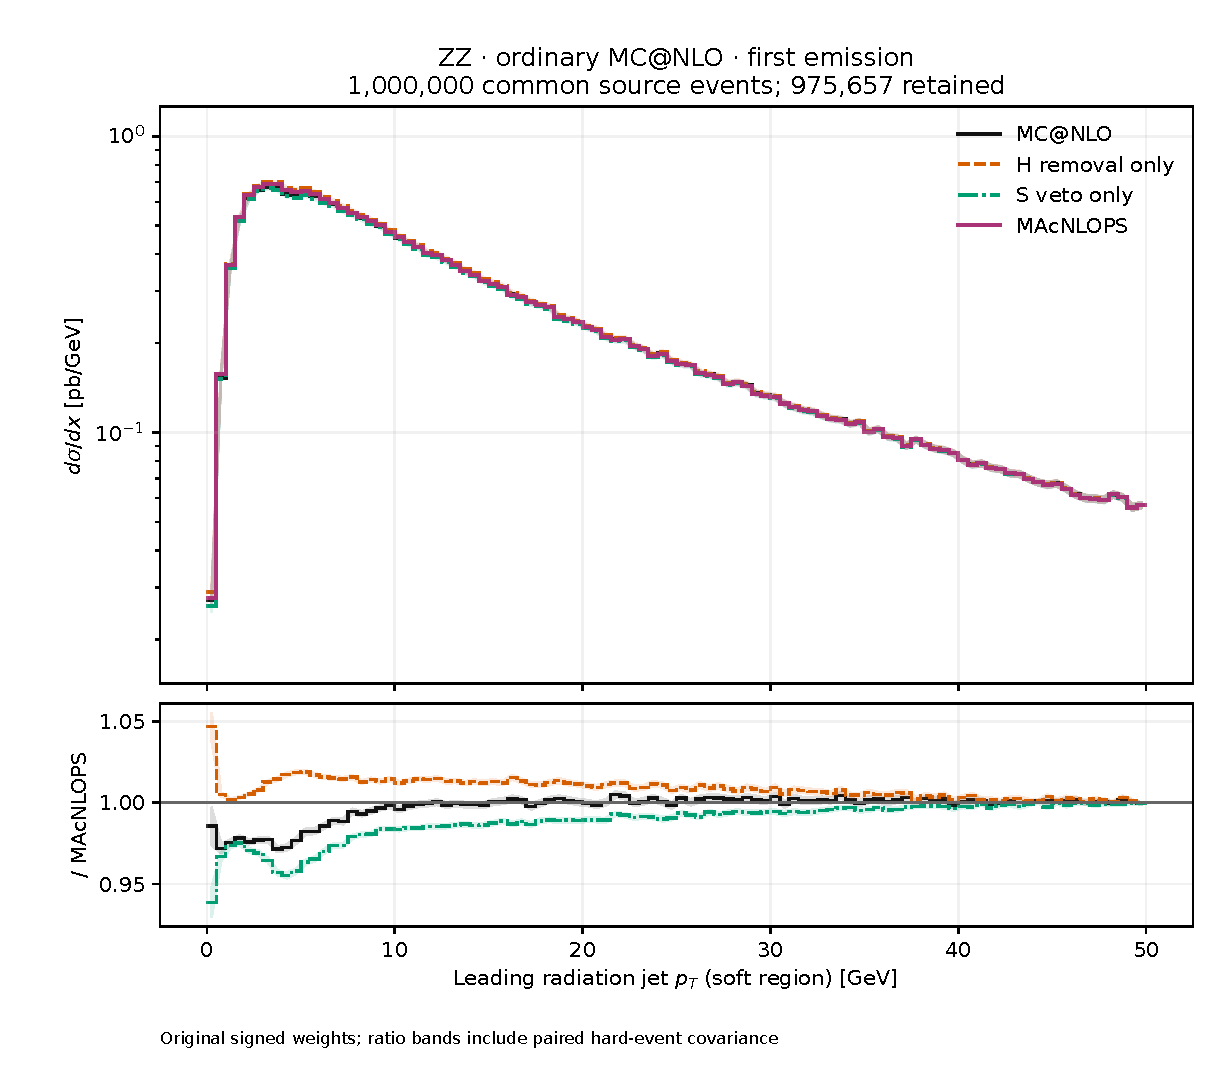
\includegraphics[width=.96\textwidth,height=.72\textheight,keepaspectratio]{figures/first/zz_ordinary/jet_pt_soft.pdf}
\caption{Global-sum campaign. ZZ (5FS), ordinary MC@NLO, first-emission proposal endpoint. The soft range is $0$--$50\GeV$ with uniform $0.5\GeV$ bins. The black curve is the complete unrejected first-step proposal control, not a separately initialized default-import shower. Orange and green isolate H removal and S veto. All ratios use the corresponding combined MAcNLOPS distribution as denominator. Original signed cross-section weights are preserved.}
\label{fig:zz-ordinary-first}
\end{figure}

\begin{figure}[p]
\centering
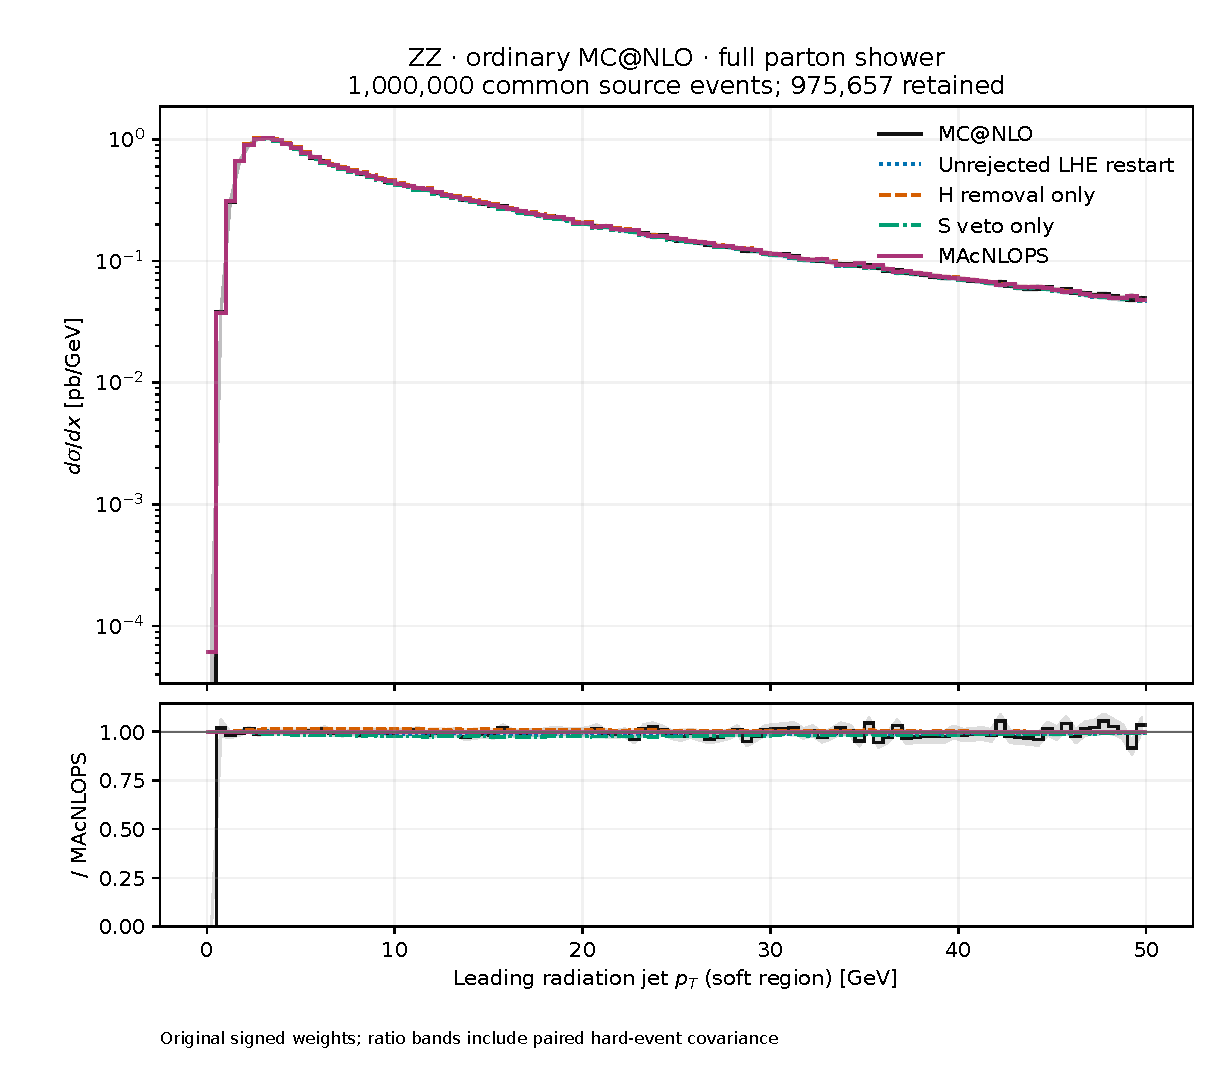
\includegraphics[width=.96\textwidth,height=.72\textheight,keepaspectratio]{figures/full/zz_ordinary/jet_pt_soft.pdf}
\caption{ZZ (5FS), ordinary MC@NLO, full parton shower. The soft range is $0$--$50\GeV$ with uniform $0.5\GeV$ bins. The black curve is the uninterrupted reference; blue is the unrejected staged restart. Orange and green isolate H removal and S veto. All ratios use the corresponding combined MAcNLOPS distribution as denominator. Original signed cross-section weights are preserved.}
\label{fig:zz-ordinary-full}
\end{figure}

\begin{figure}[p]
\centering
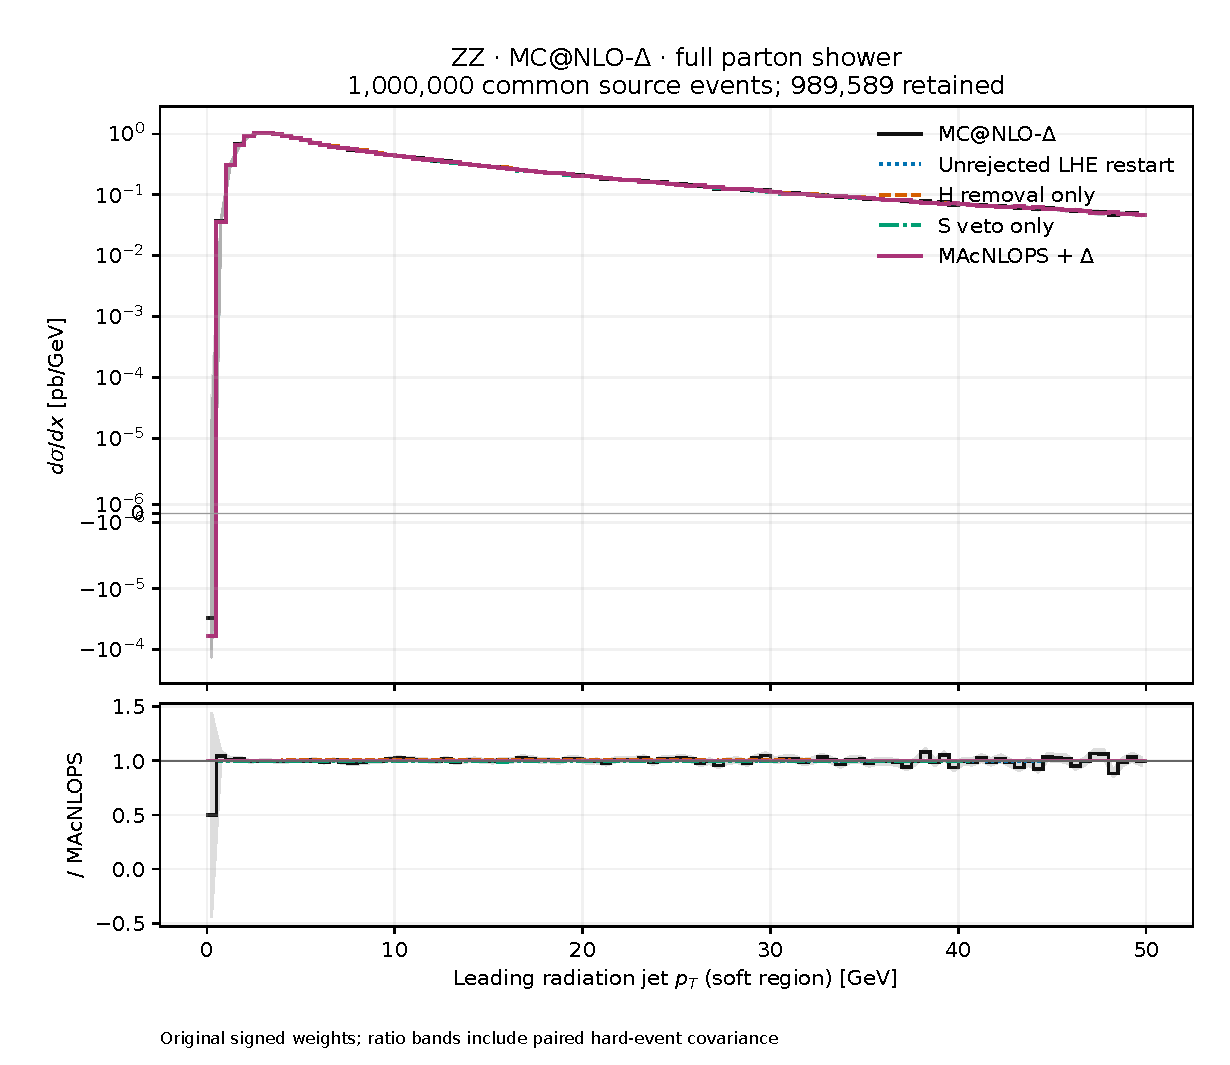
\includegraphics[width=.96\textwidth,height=.72\textheight,keepaspectratio]{figures/full/zz_delta/jet_pt_soft.pdf}
\caption{ZZ (5FS), MC@NLO-$\Delta$, full parton shower. The soft range is $0$--$50\GeV$ with uniform $0.5\GeV$ bins. The black curve is the uninterrupted reference; blue is the unrejected staged restart. Orange and green isolate H removal and S veto. All ratios use the corresponding combined MAcNLOPS distribution as denominator. Original signed cross-section weights are preserved.}
\label{fig:zz-delta-full}
\end{figure}

\begin{figure}[p]
\centering
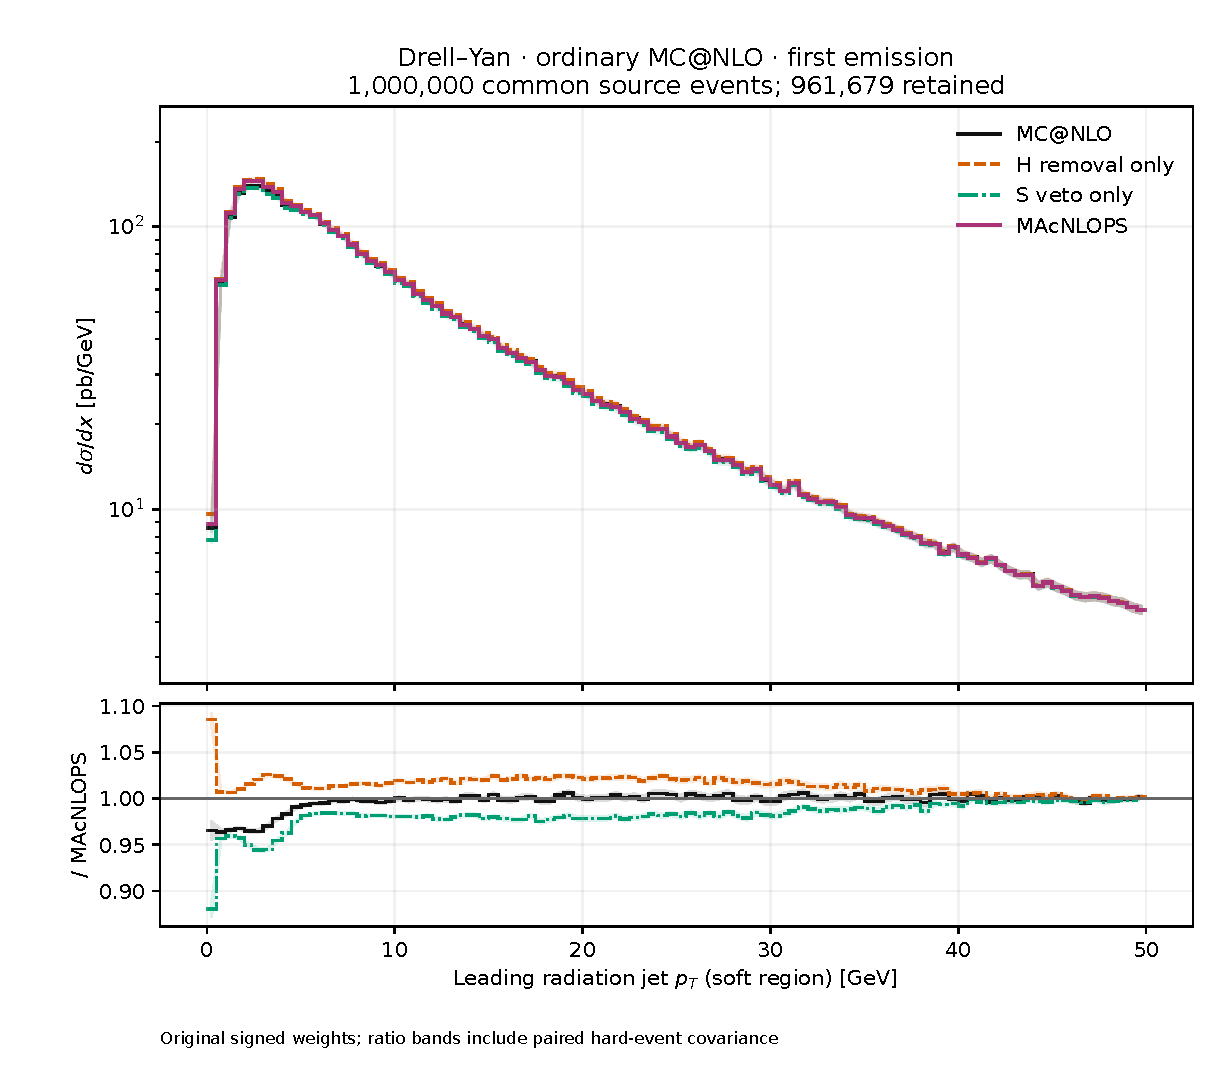
\includegraphics[width=.96\textwidth,height=.72\textheight,keepaspectratio]{figures/first/dy_ordinary/jet_pt_soft.pdf}
\caption{Drell-Yan (5FS), ordinary MC@NLO, first-emission proposal endpoint. The soft range is $0$--$50\GeV$ with uniform $0.5\GeV$ bins. The black curve is the complete unrejected first-step proposal control, not a separately initialized default-import shower. Orange and green isolate H removal and S veto. All ratios use the corresponding combined MAcNLOPS distribution as denominator. Original signed cross-section weights are preserved.}
\label{fig:dy-ordinary-first}
\end{figure}

\begin{figure}[p]
\centering
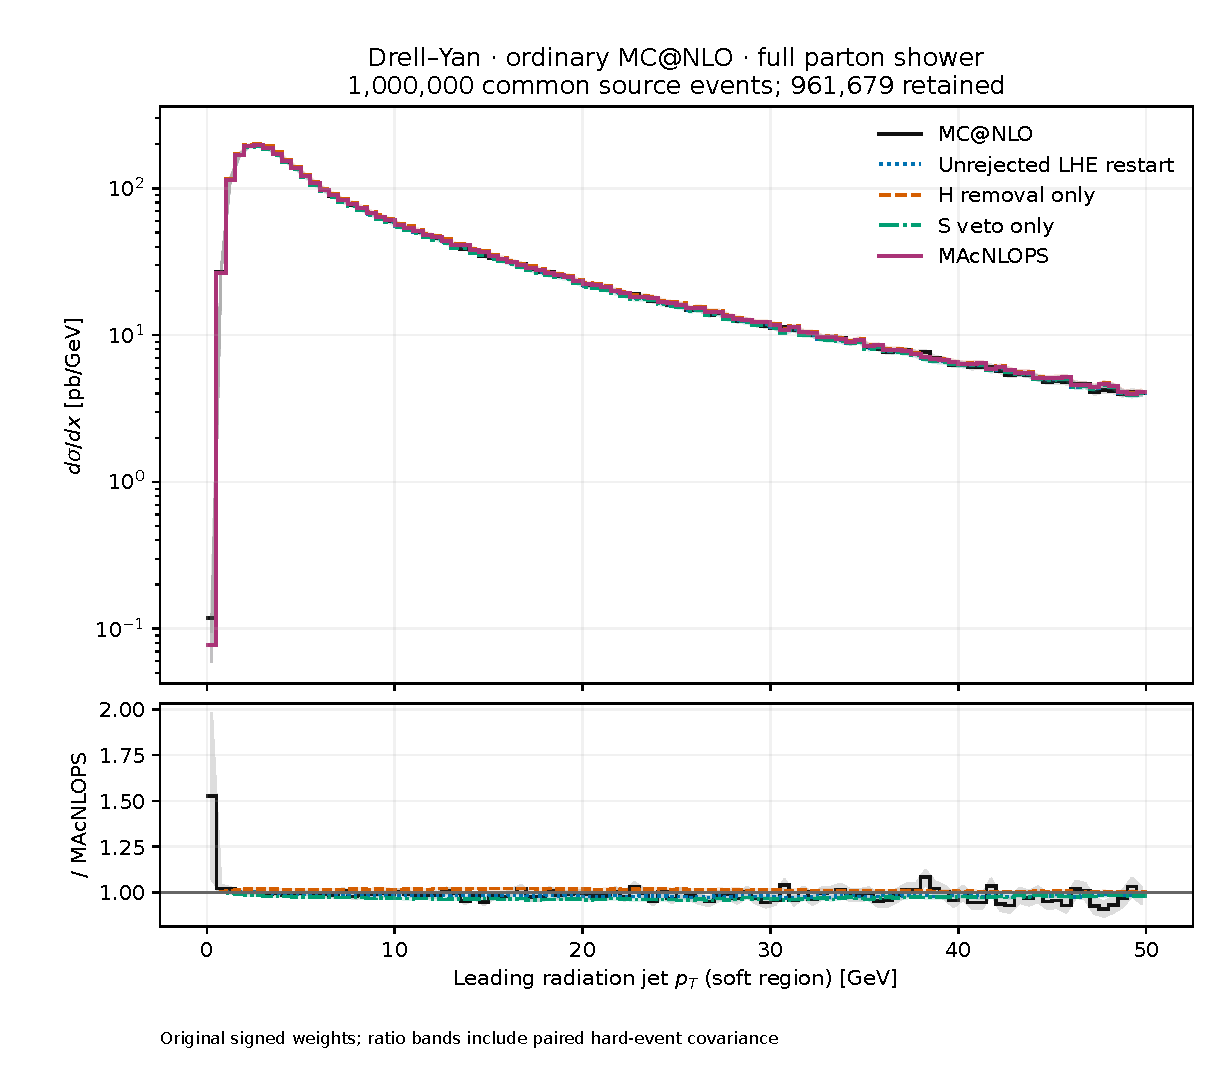
\includegraphics[width=.96\textwidth,height=.72\textheight,keepaspectratio]{figures/full/dy_ordinary/jet_pt_soft.pdf}
\caption{Global-sum campaign. Drell-Yan (5FS), ordinary MC@NLO, full parton shower. The soft range is $0$--$50\GeV$ with uniform $0.5\GeV$ bins. The black curve is the uninterrupted reference; blue is the unrejected staged restart. Orange and green isolate H removal and S veto. All ratios use the corresponding combined MAcNLOPS distribution as denominator. Original signed cross-section weights are preserved.}
\label{fig:dy-ordinary-full}
\end{figure}

\begin{figure}[p]
\centering
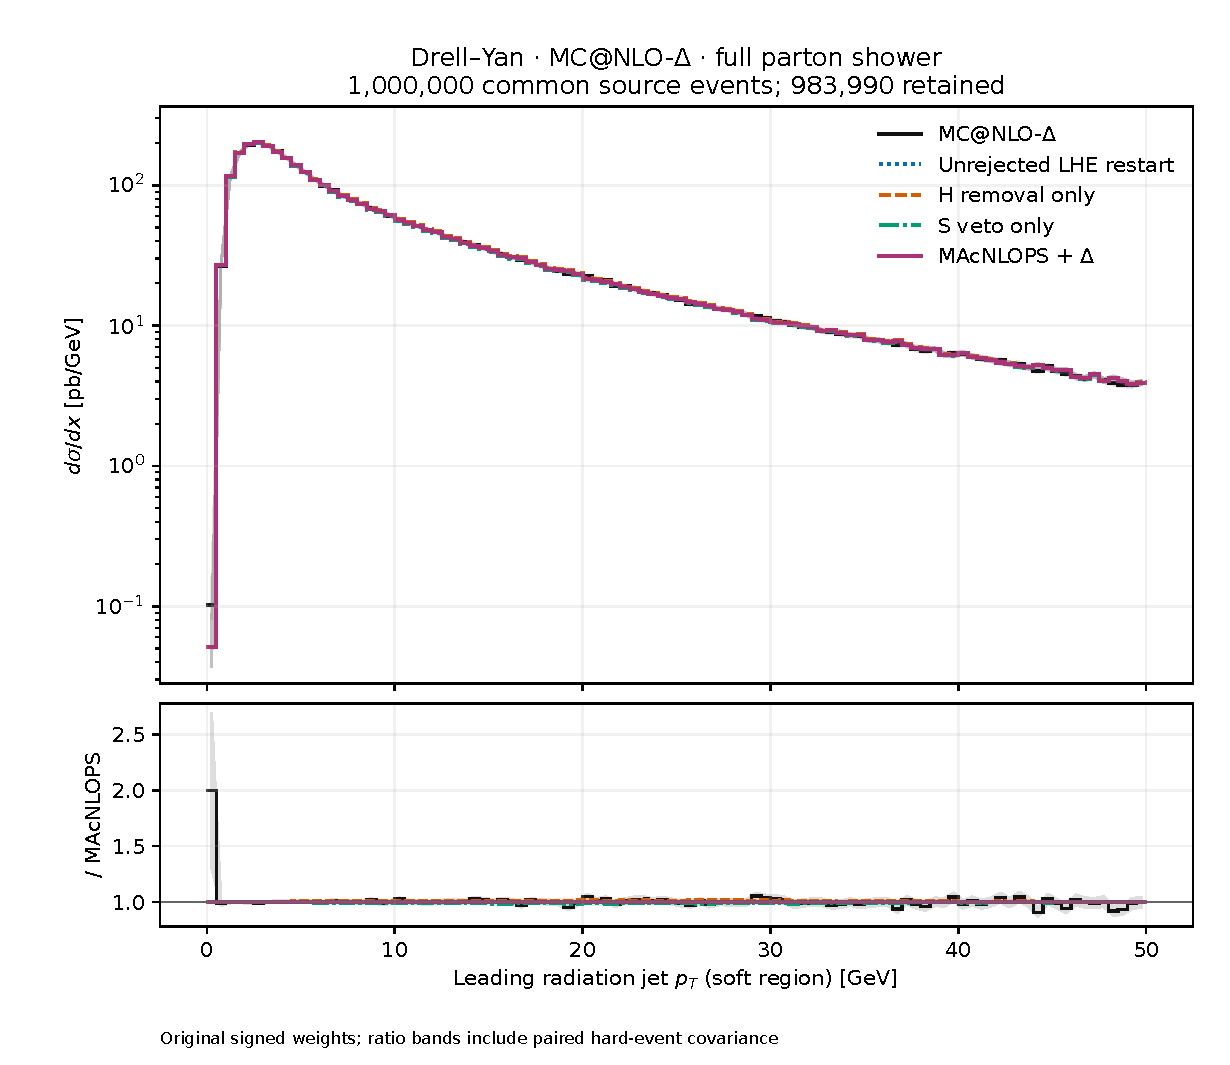
\includegraphics[width=.96\textwidth,height=.72\textheight,keepaspectratio]{figures/full/dy_delta/jet_pt_soft.pdf}
\caption{Drell-Yan (5FS), MC@NLO-$\Delta$, full parton shower. The soft range is $0$--$50\GeV$ with uniform $0.5\GeV$ bins. The black curve is the uninterrupted reference; blue is the unrejected staged restart. Orange and green isolate H removal and S veto. All ratios use the corresponding combined MAcNLOPS distribution as denominator. Original signed cross-section weights are preserved.}
\label{fig:dy-delta-full}
\end{figure}

\begin{figure}[p]
\centering
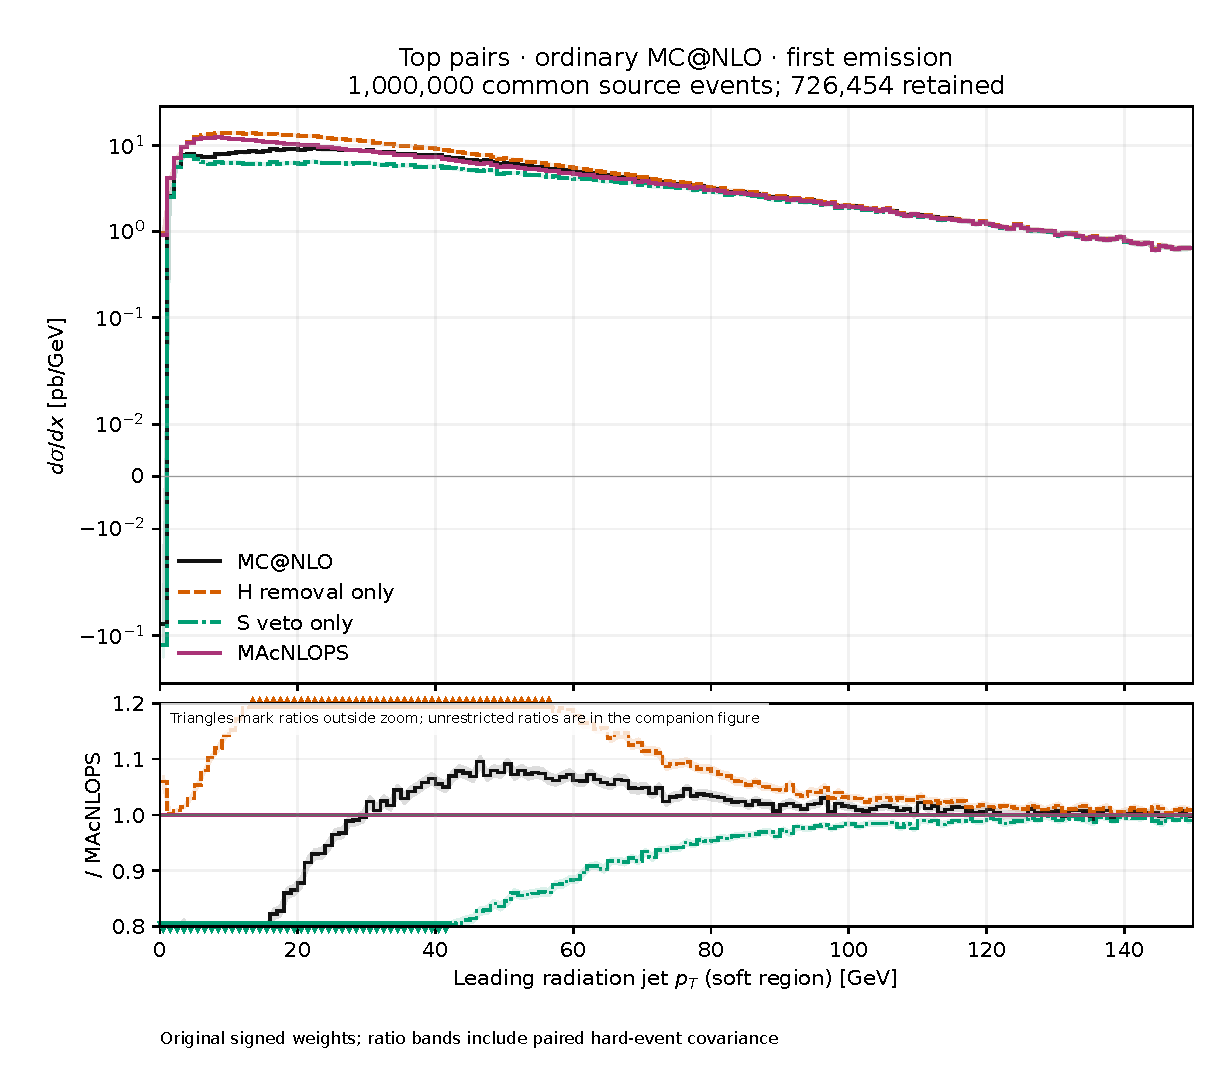
\includegraphics[width=.96\textwidth,height=.72\textheight,keepaspectratio]{figures/first/ttbar_ordinary/jet_pt_soft_ratio_zoom.pdf}
\caption{Global-sum campaign. Top pair (5FS), ordinary MC@NLO, first-emission proposal endpoint. The displayed soft range is $0$--$150\GeV$ with uniform $1\GeV$ bins. Triangles mark ratios outside the displayed zoom. The black curve is the complete unrejected first-step proposal control, not a separately initialized default-import shower. Orange and green isolate H removal and S veto. All ratios use the corresponding combined MAcNLOPS distribution as denominator. Original signed cross-section weights are preserved.}
\label{fig:ttbar-ordinary-first}
\end{figure}

\begin{figure}[p]
\centering
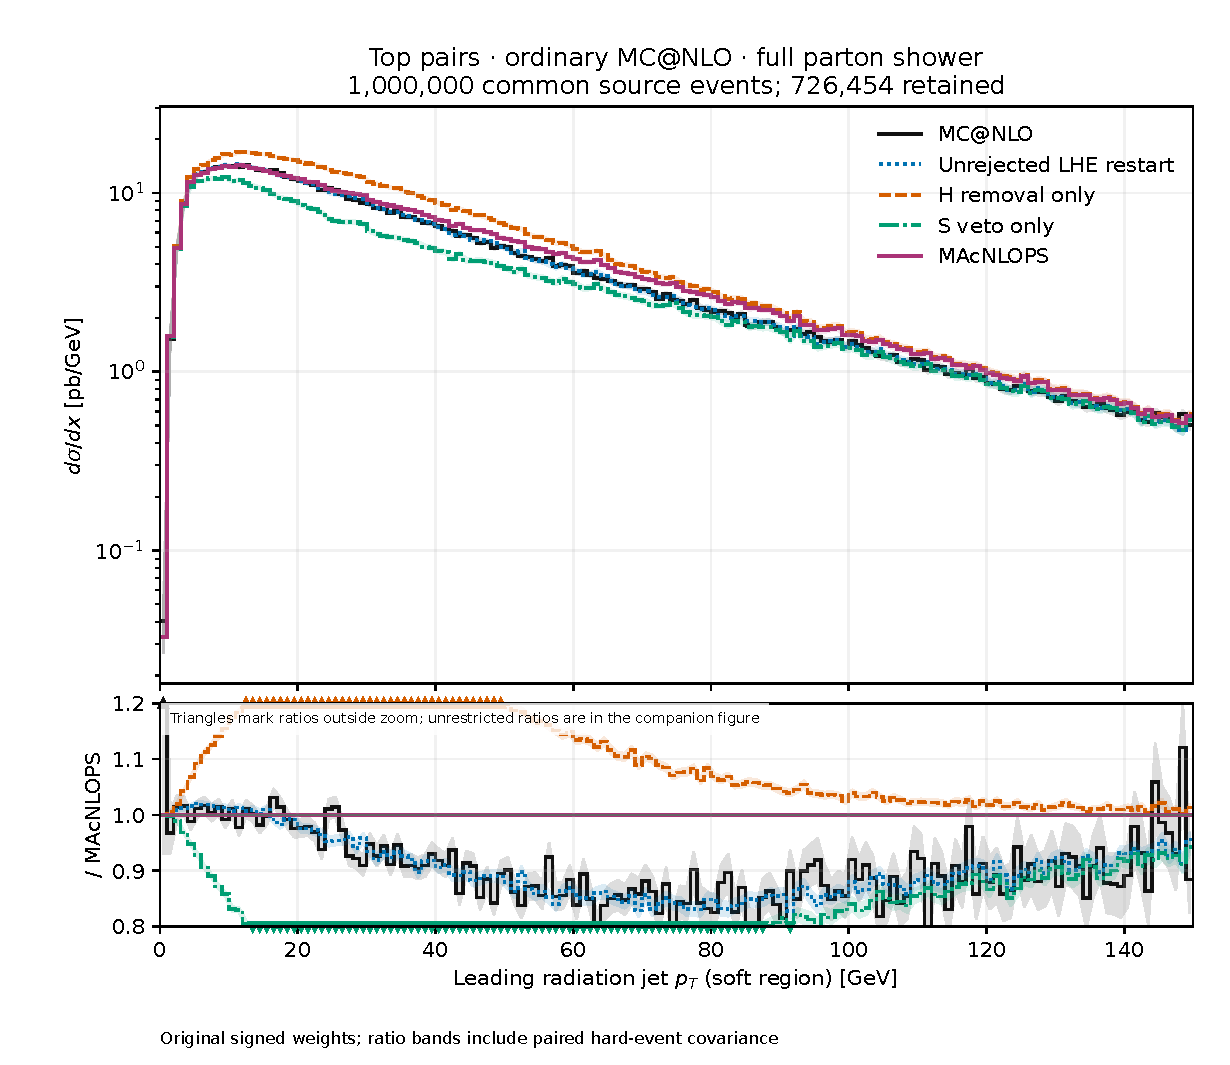
\includegraphics[width=.96\textwidth,height=.72\textheight,keepaspectratio]{figures/full/ttbar_ordinary/jet_pt_soft_ratio_zoom.pdf}
\caption{Top pair (5FS), ordinary MC@NLO, full parton shower. The displayed soft range is $0$--$150\GeV$ with uniform $1\GeV$ bins. Triangles mark ratios outside the displayed zoom. The black curve is the uninterrupted reference; blue is the unrejected staged restart. Orange and green isolate H removal and S veto. All ratios use the corresponding combined MAcNLOPS distribution as denominator. Original signed cross-section weights are preserved.}
\label{fig:ttbar-ordinary-full}
\end{figure}

\begin{figure}[p]
\centering
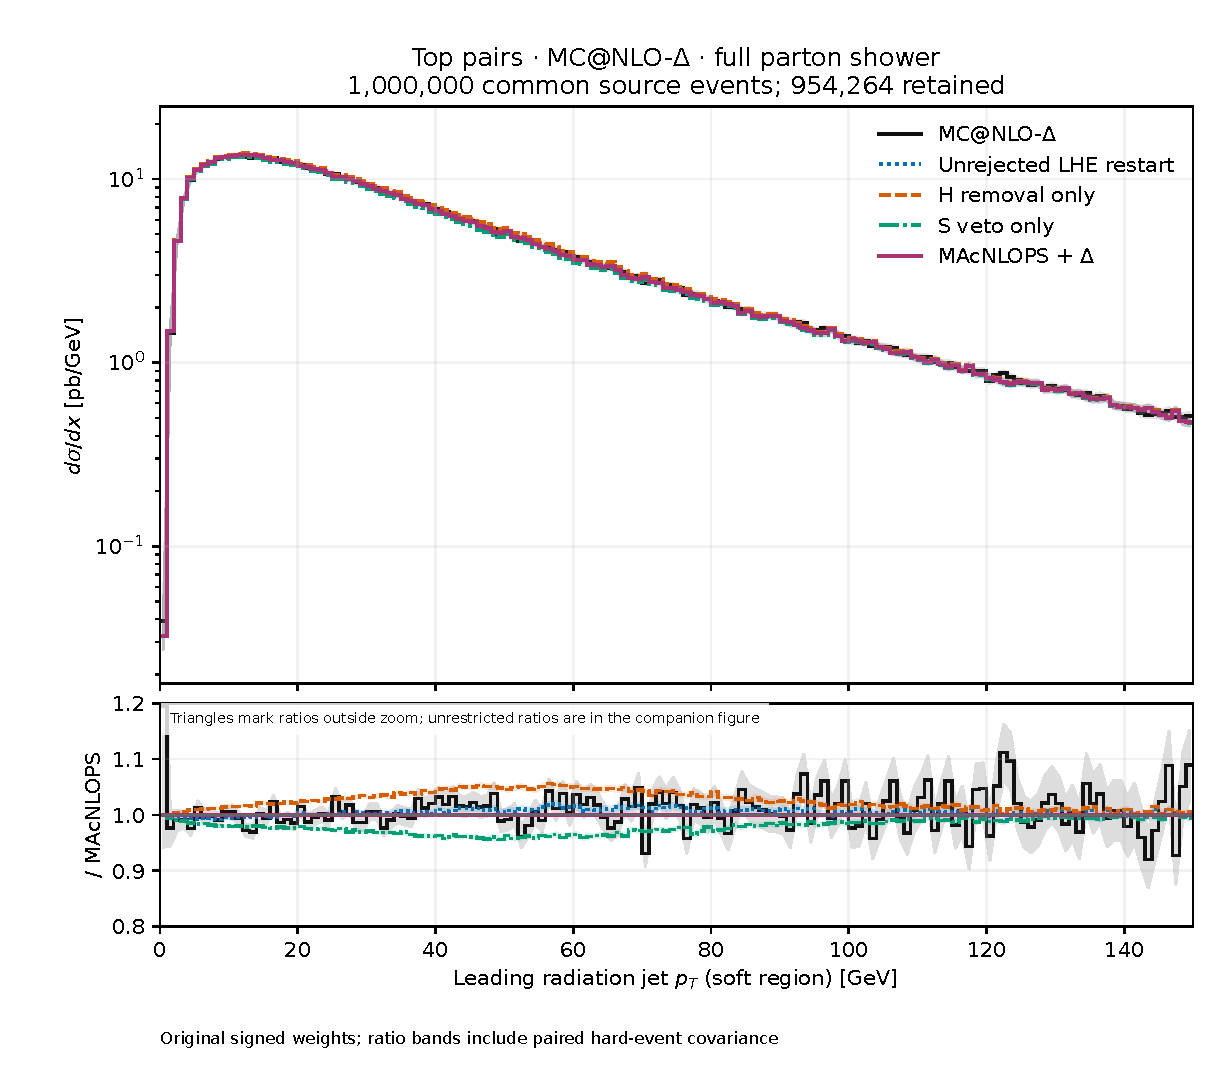
\includegraphics[width=.96\textwidth,height=.72\textheight,keepaspectratio]{figures/full/ttbar_delta/jet_pt_soft_ratio_zoom.pdf}
\caption{Global-sum campaign. Top pair (5FS), MC@NLO-$\Delta$, full parton shower. The displayed soft range is $0$--$150\GeV$ with uniform $1\GeV$ bins. Triangles mark ratios outside the displayed zoom. The black curve is the uninterrupted reference; blue is the unrejected staged restart. Orange and green isolate H removal and S veto. All ratios use the corresponding combined MAcNLOPS distribution as denominator. Original signed cross-section weights are preserved.}
\label{fig:ttbar-delta-full}
\end{figure}

\begin{figure}[p]
\centering
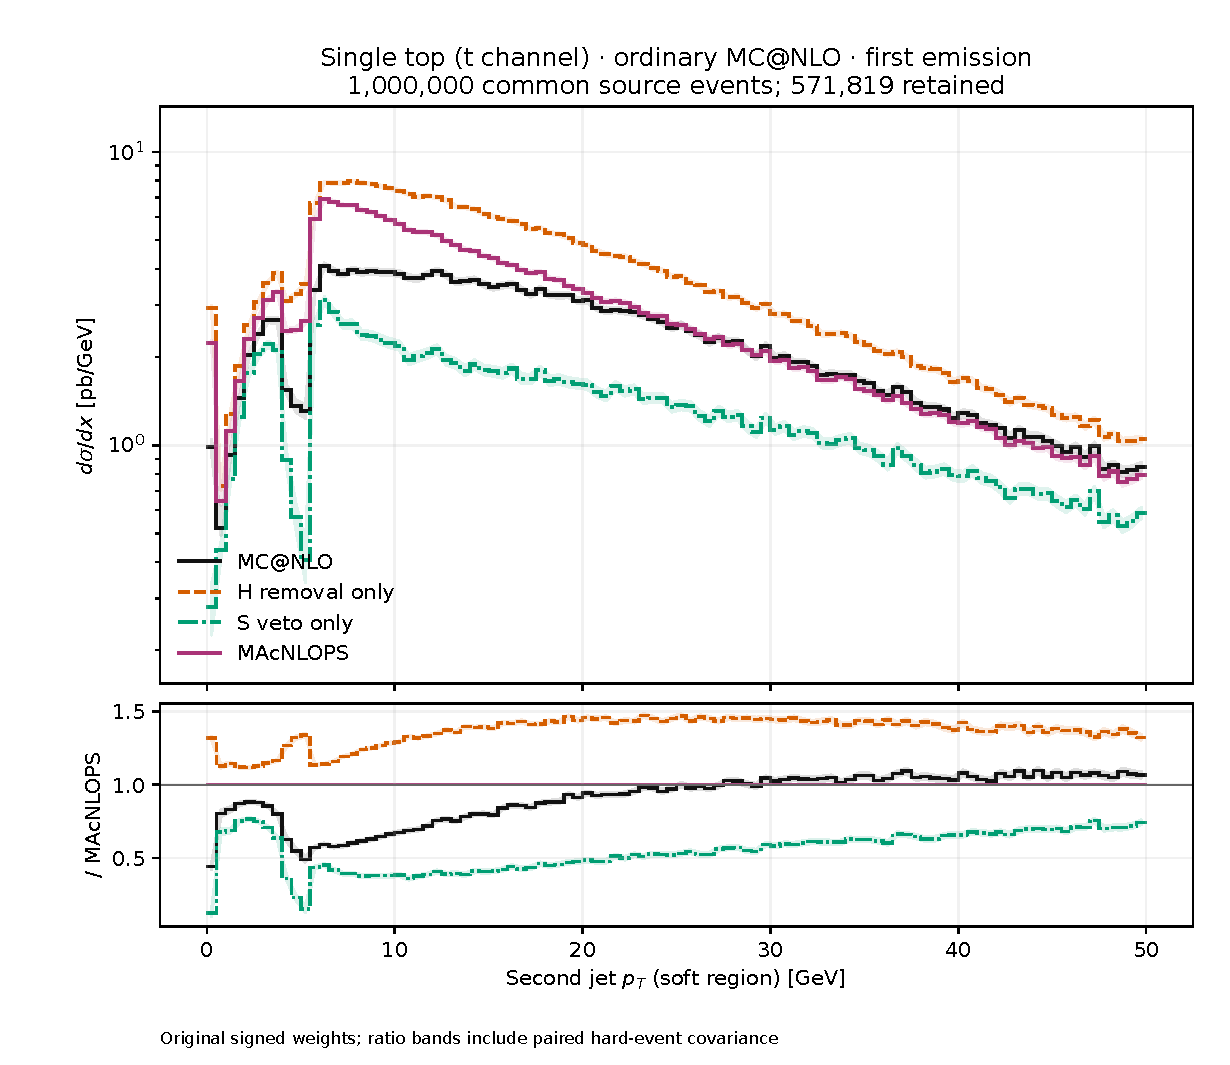
\includegraphics[width=.96\textwidth,height=.72\textheight,keepaspectratio]{figures/first/single_top_ordinary/jet_pt_soft.pdf}
\caption{Single top (5FS), ordinary MC@NLO, first-emission proposal endpoint. The second inclusive jet is shown; the leading jet is the spectator proxy. The soft range is $0$--$50\GeV$ with uniform $0.5\GeV$ bins. The black curve is the complete unrejected first-step proposal control, not a separately initialized default-import shower. Orange and green isolate H removal and S veto. All ratios use the corresponding combined MAcNLOPS distribution as denominator. Original signed cross-section weights are preserved.}
\label{fig:single_top-ordinary-first}
\end{figure}

\begin{figure}[p]
\centering
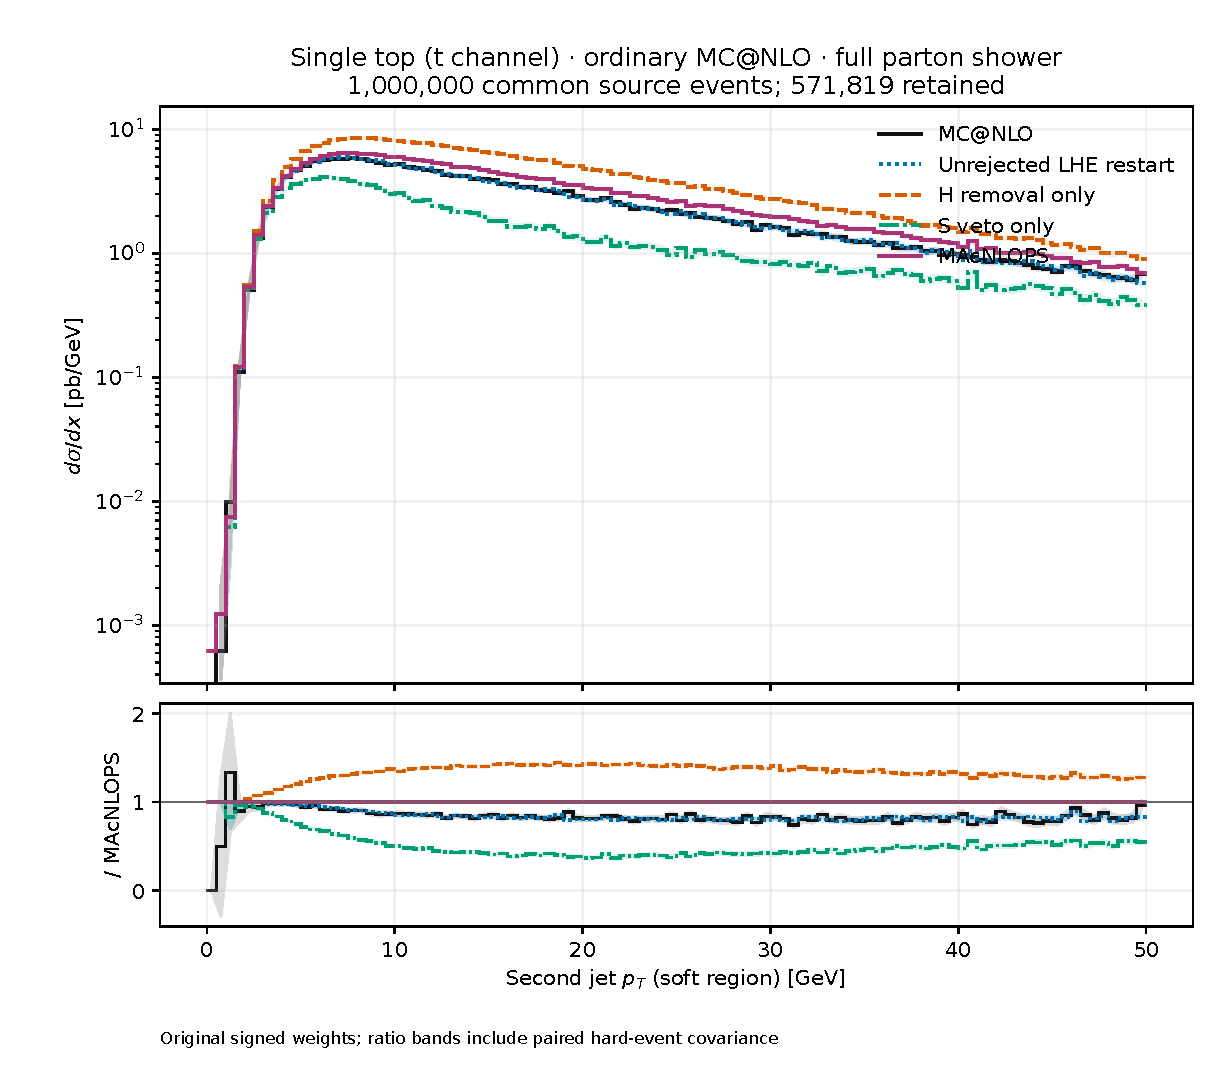
\includegraphics[width=.96\textwidth,height=.72\textheight,keepaspectratio]{figures/full/single_top_ordinary/jet_pt_soft.pdf}
\caption{Global-sum campaign. Single top (5FS), ordinary MC@NLO, full parton shower. The second inclusive jet is shown; the leading jet is the spectator proxy. The soft range is $0$--$50\GeV$ with uniform $0.5\GeV$ bins. The black curve is the uninterrupted reference; blue is the unrejected staged restart. Orange and green isolate H removal and S veto. All ratios use the corresponding combined MAcNLOPS distribution as denominator. Original signed cross-section weights are preserved.}
\label{fig:single_top-ordinary-full}
\end{figure}

\begin{figure}[p]
\centering
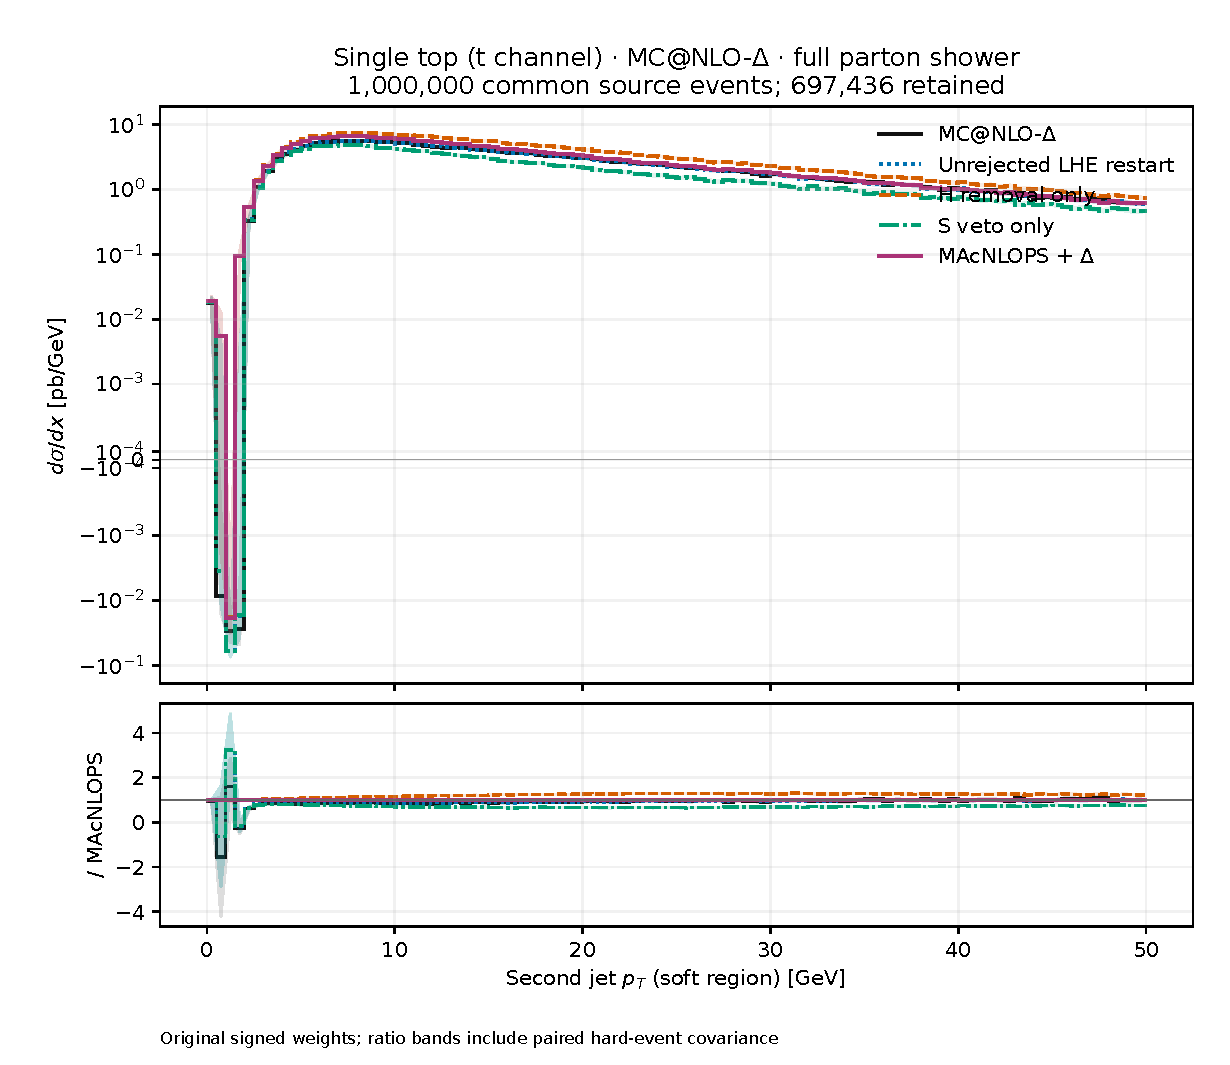
\includegraphics[width=.96\textwidth,height=.72\textheight,keepaspectratio]{figures/full/single_top_delta/jet_pt_soft.pdf}
\caption{Global-sum campaign. Single top (5FS), MC@NLO-$\Delta$, full parton shower. The second inclusive jet is shown; the leading jet is the spectator proxy. The soft range is $0$--$50\GeV$ with uniform $0.5\GeV$ bins. The black curve is the uninterrupted reference; blue is the unrejected staged restart. Orange and green isolate H removal and S veto. All ratios use the corresponding combined MAcNLOPS distribution as denominator. Original signed cross-section weights are preserved.}
\label{fig:single_top-delta-full}
\end{figure}

\begin{figure}[p]
\centering
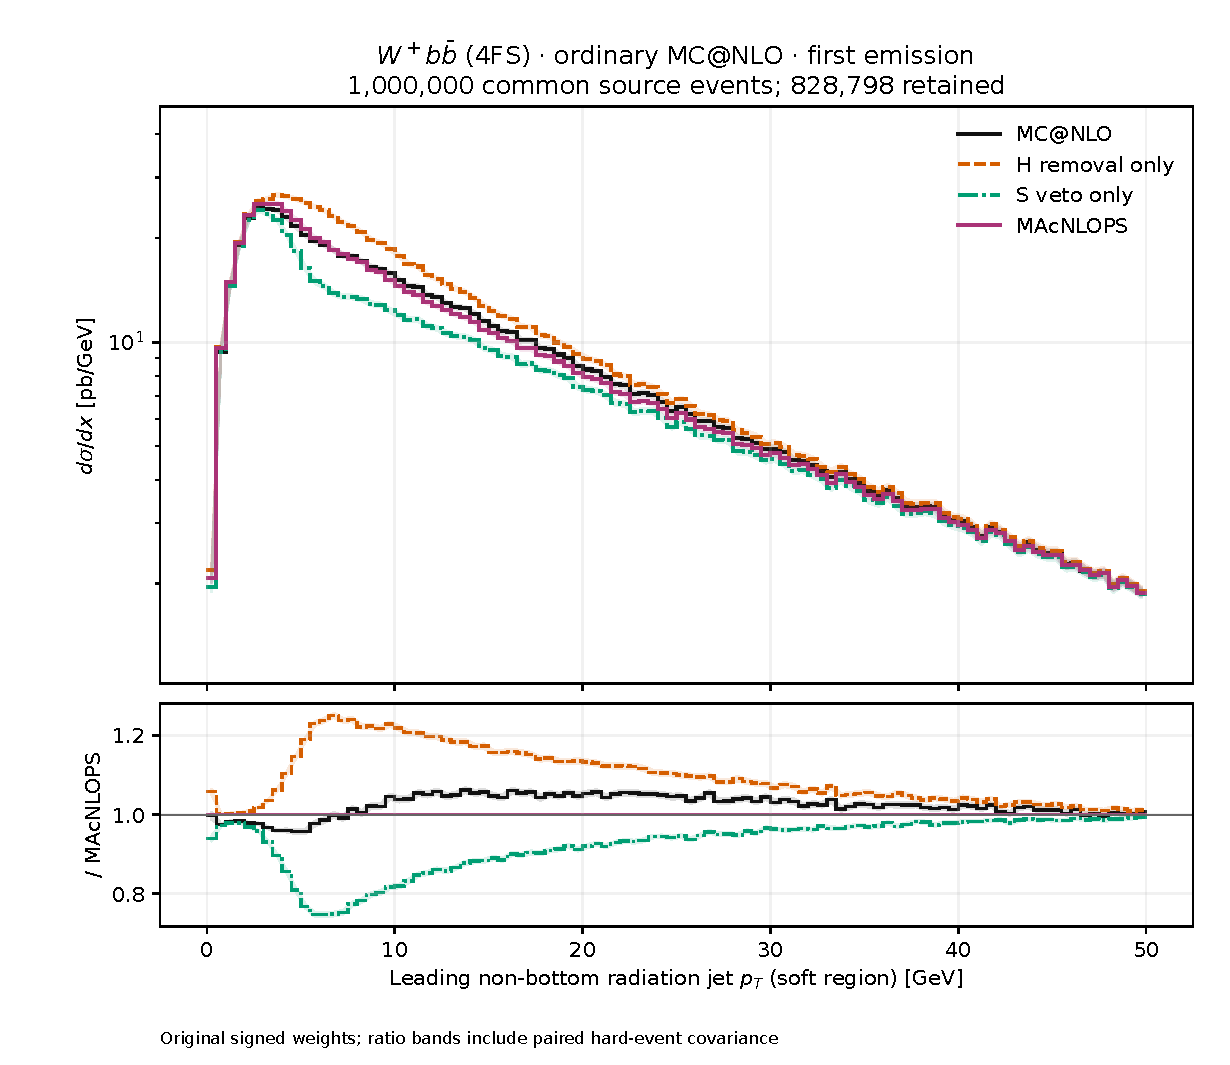
\includegraphics[width=.96\textwidth,height=.72\textheight,keepaspectratio]{figures/first/wbb_ordinary/jet_pt_soft.pdf}
\caption{Global-sum campaign. Wbb (4FS), ordinary MC@NLO, first-emission proposal endpoint. The radiation jets exclude stable bottom partons before clustering. The soft range is $0$--$50\GeV$ with uniform $0.5\GeV$ bins. The black curve is the complete unrejected first-step proposal control, not a separately initialized default-import shower. Orange and green isolate H removal and S veto. All ratios use the corresponding combined MAcNLOPS distribution as denominator. Original signed cross-section weights are preserved.}
\label{fig:wbb-ordinary-first}
\end{figure}

\begin{figure}[p]
\centering
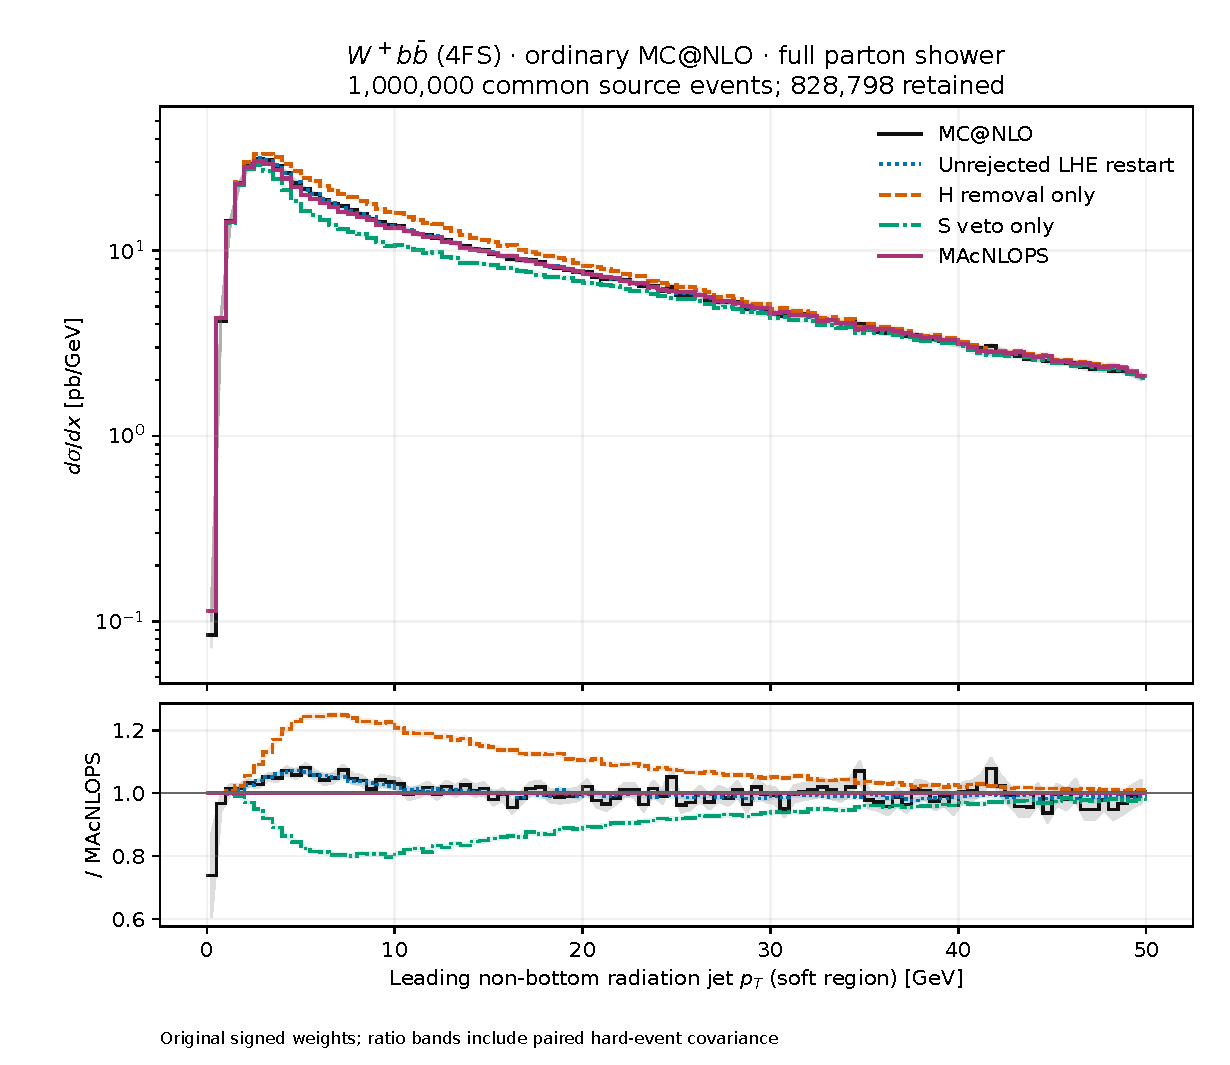
\includegraphics[width=.96\textwidth,height=.72\textheight,keepaspectratio]{figures/full/wbb_ordinary/jet_pt_soft.pdf}
\caption{Wbb (4FS), ordinary MC@NLO, full parton shower. The radiation jets exclude stable bottom partons before clustering. The soft range is $0$--$50\GeV$ with uniform $0.5\GeV$ bins. The black curve is the uninterrupted reference; blue is the unrejected staged restart. Orange and green isolate H removal and S veto. All ratios use the corresponding combined MAcNLOPS distribution as denominator. Original signed cross-section weights are preserved.}
\label{fig:wbb-ordinary-full}
\end{figure}

\begin{figure}[p]
\centering
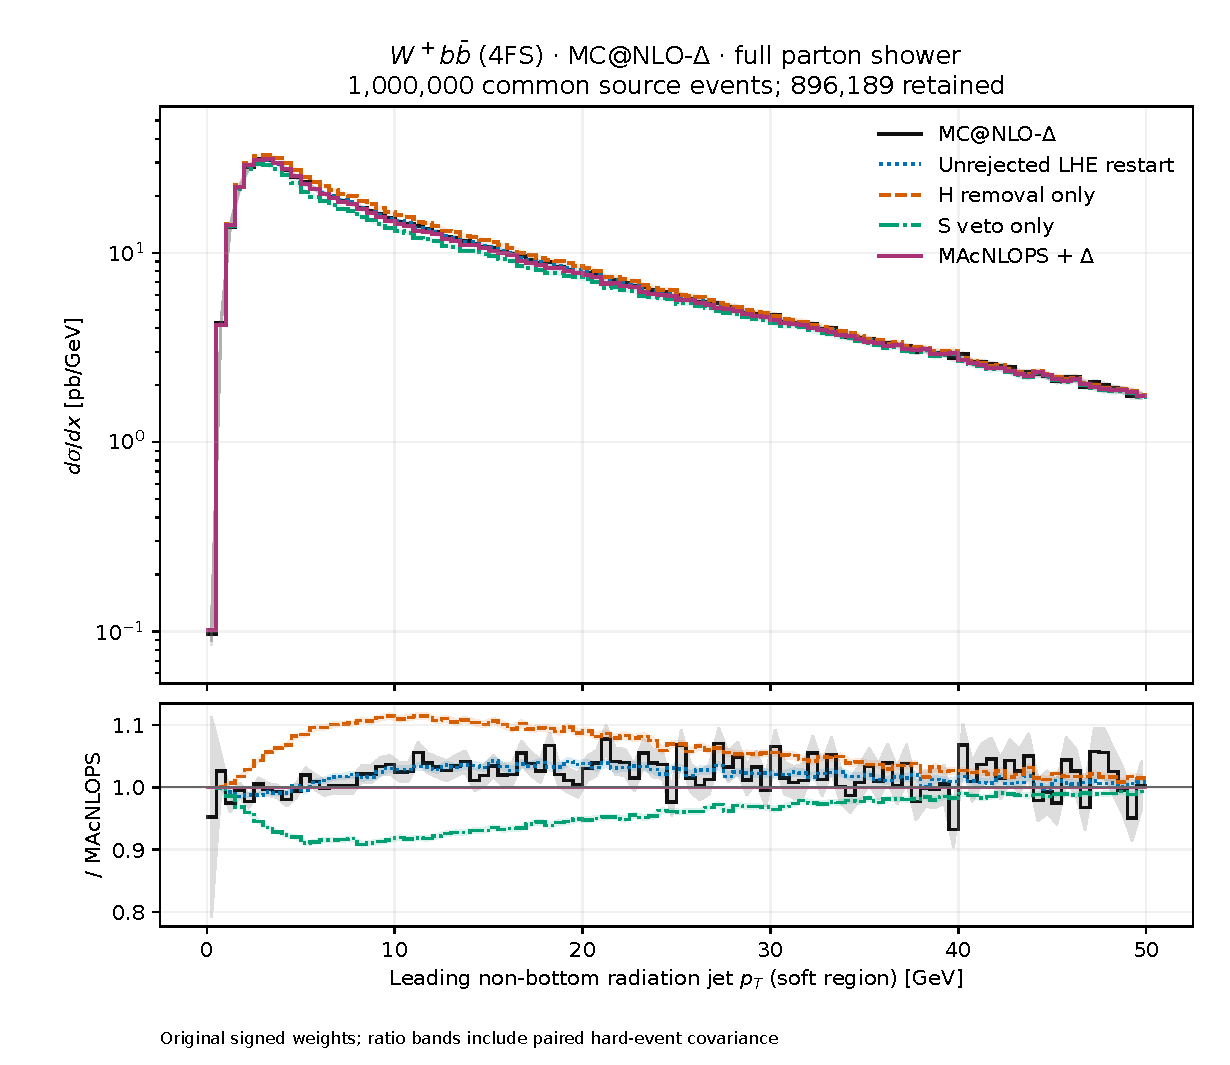
\includegraphics[width=.96\textwidth,height=.72\textheight,keepaspectratio]{figures/full/wbb_delta/jet_pt_soft.pdf}
\caption{Global-sum campaign. Wbb (4FS), MC@NLO-$\Delta$, full parton shower. The radiation jets exclude stable bottom partons before clustering. The soft range is $0$--$50\GeV$ with uniform $0.5\GeV$ bins. The black curve is the uninterrupted reference; blue is the unrejected staged restart. Orange and green isolate H removal and S veto. All ratios use the corresponding combined MAcNLOPS distribution as denominator. Original signed cross-section weights are preserved.}
\label{fig:wbb-delta-full}
\end{figure}

\FloatBarrier

\section{Conclusions and the remaining accuracy conditions}
\label{sec:conclusions}
The implementation provides a multi-step construction: qualified source
generation, canonical first-step proposals, bounded whole-event H
removal/S veto, randomized accepted LHE collection and scale-preserving
continuation. The current sampled mode retains the native history,
Born integration diagram and colour flow before sign classification.
The S event's actual branching identifies its native emission component;
its original integration owner does not constrain the shower radiator.
Diagram and oriented-flow indices are transported under certified
identical-Born-leg permutations, with the corresponding statistical
normalization applied to all densities.

Ordinary matching keeps the generated bogus-Sudakov multiplier:
its transferred numerator is $[P_a(D_{G,a}-R_a)]_+$. Sampled Delta
matching uses the undamped completed numerator $u_a=[D_{G,a}-R_a]_+$
and rejects eligible S events with probability
$\min(u_a/K_a,1)$. The original negative H measure is still
$\Delta_a u_a$, and the residual is $\Delta_a[u_a-K_a]_+$.
This consistent pair removes the need for numerical source-Delta
evaluation at S emissions. It does not replace the G completion by a
scalar shower kernel or divide Delta out of the nominal event weight.
The global-sum compatibility mode retains its original source-damped
ratio and different residual; both prescriptions are explicitly labelled
in the accepted files and reports.

The source G completion, ordinary fixed low-scale factor, physical
shower Sudakov and Delta source factor remain distinct. Hard and MC
mass conventions are recorded separately, and the written first-emission
endpoint carries its own current shower bounds. The finite transfer is
governed by its actual signed S emission density. On the sampled Delta
component space it is
$C_{0,a}[\overline\Delta_a-E_{g,a}^{\Delta}/K_a]$.
Retaining components resolves the nonlinear mixed-history sign problem;
it does not impose equality of the source and physical shower measures.
Negative S coefficients, insufficient support, G/kernel differences,
source-scale mixtures and different continuation laws remain relevant.

The completed ten-million-source-event campaign used the global-sum
prescription. Its count, weight, covariance and kinematic checks passed,
and it exhibits sizeable finite differences for some processes. All
703 figure assets are retained, with campaign labels that prevent their
interpretation as sampled-mode results. Focused native closure, identical
gluon, support-boundary and small-source checks exercise the new
implementation, including genuine negative-H removal and S veto. They
are implementation evidence rather than a new precision production or
a measurement of the sampled prescription's finite distribution defect.

An exact endpoint cancellation would require the actual positive or
signed eligible S density in the same component space, adequate common
support and the corresponding source negative measure. Equality after
further showering additionally requires equality of the transferred
full states under the continuation law. A perturbative accuracy argument
needs the leading native-law/kernel correspondence; its expected order
cannot establish that correspondence or bound logarithmically enhanced
finite effects. The retained source labels, explicit mechanism controls,
portable profiles and complete figure archive make those conditions
stated and testable, without normalizing away the observed differences.

\FloatBarrier
\bibliographystyle{unsrtnat}
\bibliography{references}
\clearpage
\appendix
\section{Notation and reproducibility record}
\label{sec:notation}
\begin{longtable}{p{.18\textwidth}p{.76\textwidth}}
\toprule
Symbol & Meaning\\\midrule\endhead
$q,b_h,r_h$ & Labelled real point, the Born projection of history $h$, and its radiation coordinates.\\
$J_h$ & Positive conversion of a native Born/radiation measure to the common real measure.\\
$R,H,D_{\rm eff}$ & Real density, actual generated hard density, and effective transfer $R-H$.\\
$H_-$ & Negative part $[-H]_+$ taken after the required physical source sum; not generally a sum of negative parts.\\
$K_g$ & Eligible positive scalar leading shower density. It contains support and starting-scale marginals, not an actual emission Sudakov.\\
$C$ & Bounded transfer $\min(H_-,K_g)$ in the ordinary scalar construction.\\
$a_S,a_H^-$ & Acceptance of an eligible emitted S event and of a negative H event.\\
$E_g$ & Actual signed cross-section density of eligible first S emissions, including the source S weights and native shower law.\\
$E_g^+$ & Corresponding positive-weight S density, used only in the alternative exact-cancellation discussion.\\
$G;g_s,g_c,g_\phi,\widetilde g_s$ & Source G-function controls and effective completion factors, distinct from event/history eligibility $g,g_h$; these are not branching probabilities.\\
$P$ & Actual low-scale source multiplier, including the ordinary artificial bogus factor or its Delta replacement where appropriate.\\
$\Delta_{\rm PS}$ & Physical conditional shower no-harder-emission probability.\\
$\Delta_{\rm src}$ & Delta source factor/context; not the actual first-emission Sudakov of the vetoed S event.\\
$ij$ & Outer FKS sector, with unresolved leg $i$ and sister $j$, in source organization.\\
$kl$ & Native emitted/emitter-history label of the explicit MC-history sum; not a Born-colour-flow label.\\
$c,\ell$ & Born-colour flow and the separate colour-connection label for a selected native history/flow.\\
$p_c,q_c$ & Physical flow fraction and its Monte Carlo sampling probability; their roles must not be counted twice.\\
$\zeta,\lambda,z$ & Actual S source/shower state, fresh Delta source-H auxiliary variables, and complete post-first-step state, respectively.\\
\bottomrule
\end{longtable}

The base revision is
\code{\detokenize{e96e7f4eac0aa3b4dc6ab58049d729462b64d76e}} with a
modified working tree. It is not identified with an unmodified tagged
release. \code{\detokenize{evidence_manifest.json}} records source hashes,
the completed dataset checks and the data-collection time;
\code{\detokenize{implementation_changes.patch}} records the tracked
implementation differences. Runtime source manifests, archived
per-source cards and the two single-top recovery records determine the
actual production provenance, which is more specific than the base Git
revision alone.

\code{\detokenize{paper_data.json}} freezes the numerical records used
for the tables. \code{\detokenize{figure_manifest.json}} identifies every
included current and historical figure. The source archive contains all
LaTeX files, the bibliography, generated tables and figure PDFs, so
rebuilding the document needs neither the LHE files nor a new shower.
It is a reproducible document bundle, not a substitute for distributing
the much larger event-generation campaign and all installed libraries.

To rebuild, use \code{make paper} for the narrative edition and
\code{make complete} for the edition containing the full atlas.
\code{make atlas} builds the standalone figure atlas. The optional
\code{make refresh} reads the original completed campaign to regenerate
the frozen tables and copies; it performs no event generation or
showering and is unnecessary for an ordinary LaTeX rebuild.

The document checks distinguish three levels of evidence: algebraic
identities of the stated transfer, successful implementation/data
consistency checks, and conditions still needed for an accuracy theorem.
Counts and histogram identities cannot supply the missing native-density
proof; an expected perturbative order cannot replace the observed
finite differences. That distinction applies equally to the current
plots and to the separately labelled historical material.

\ifallfigures
\clearpage
\section{Complete figure atlas}
\label{sec:atlas}
This appendix contains every plot PDF in the completed million-event
campaign: 696 panels, including the unrestricted and zoomed ratio
versions and all separate mechanism panels. The 20-page overview books
are selections of these same panels and are not duplicated as additional
datasets. Fifteen panels are also repeated in the main text to support
the discussion. Each atlas panel retains its original vector-PDF size;
the PDF bookmarks identify the process, source, shower level, observable
and variant. In the 696 current panels, main and mechanism ratios are relative to the
corresponding combined \macnlops{} result. The raw numerical histograms
and covariance arrays remain in the validation directories.

The final seven panels reproduce the earlier paper's archived figures
from 20 October 2026. They are visibly marked historical. That study used
200,000-event samples and a different, patched shower/runtime workflow;
their original ratio conventions, including normalization to the
unrejected source, are retained. Those panels are included for completeness, not combined with the
million-event results or used as validation of the current restart.
The list and SHA256 of every included PDF are in
\code{\detokenize{figure_manifest.json}}.
\clearpage
\includepdf[pages=1,fitpaper=true,pagecommand={\thispagestyle{empty}\pdfbookmark[1]{First emission / ZZ (5FS) / ordinary}{atlas-group-1}\pdfbookmark[2]{delta phi / standard}{atlas-figure-1}}]{figures/first/zz_ordinary/delta_phi.pdf}
\includepdf[pages=1,fitpaper=true,pagecommand={\thispagestyle{empty}\pdfbookmark[2]{delta phi deficit / standard}{atlas-figure-2}}]{figures/first/zz_ordinary/delta_phi_deficit.pdf}
\includepdf[pages=1,fitpaper=true,pagecommand={\thispagestyle{empty}\pdfbookmark[2]{delta phi deficit / ratio zoom}{atlas-figure-3}}]{figures/first/zz_ordinary/delta_phi_deficit_ratio_zoom.pdf}
\includepdf[pages=1,fitpaper=true,pagecommand={\thispagestyle{empty}\pdfbookmark[2]{delta phi / ratio zoom}{atlas-figure-4}}]{figures/first/zz_ordinary/delta_phi_ratio_zoom.pdf}
\includepdf[pages=1,fitpaper=true,pagecommand={\thispagestyle{empty}\pdfbookmark[2]{delta y / standard}{atlas-figure-5}}]{figures/first/zz_ordinary/delta_y.pdf}
\includepdf[pages=1,fitpaper=true,pagecommand={\thispagestyle{empty}\pdfbookmark[2]{delta y / ratio zoom}{atlas-figure-6}}]{figures/first/zz_ordinary/delta_y_ratio_zoom.pdf}
\includepdf[pages=1,fitpaper=true,pagecommand={\thispagestyle{empty}\pdfbookmark[2]{jet pt / standard}{atlas-figure-7}}]{figures/first/zz_ordinary/jet_pt.pdf}
\includepdf[pages=1,fitpaper=true,pagecommand={\thispagestyle{empty}\pdfbookmark[2]{jet pt / mechanisms}{atlas-figure-8}}]{figures/first/zz_ordinary/jet_pt_mechanisms.pdf}
\includepdf[pages=1,fitpaper=true,pagecommand={\thispagestyle{empty}\pdfbookmark[2]{jet pt / ratio zoom}{atlas-figure-9}}]{figures/first/zz_ordinary/jet_pt_ratio_zoom.pdf}
\includepdf[pages=1,fitpaper=true,pagecommand={\thispagestyle{empty}\pdfbookmark[2]{jet pt soft / standard}{atlas-figure-10}}]{figures/first/zz_ordinary/jet_pt_soft.pdf}
\includepdf[pages=1,fitpaper=true,pagecommand={\thispagestyle{empty}\pdfbookmark[2]{jet pt soft / mechanisms}{atlas-figure-11}}]{figures/first/zz_ordinary/jet_pt_soft_mechanisms.pdf}
\includepdf[pages=1,fitpaper=true,pagecommand={\thispagestyle{empty}\pdfbookmark[2]{jet pt soft / ratio zoom}{atlas-figure-12}}]{figures/first/zz_ordinary/jet_pt_soft_ratio_zoom.pdf}
\includepdf[pages=1,fitpaper=true,pagecommand={\thispagestyle{empty}\pdfbookmark[2]{jet y / standard}{atlas-figure-13}}]{figures/first/zz_ordinary/jet_y.pdf}
\includepdf[pages=1,fitpaper=true,pagecommand={\thispagestyle{empty}\pdfbookmark[2]{jet y / ratio zoom}{atlas-figure-14}}]{figures/first/zz_ordinary/jet_y_ratio_zoom.pdf}
\includepdf[pages=1,fitpaper=true,pagecommand={\thispagestyle{empty}\pdfbookmark[2]{object 1 pt / standard}{atlas-figure-15}}]{figures/first/zz_ordinary/object_1_pt.pdf}
\includepdf[pages=1,fitpaper=true,pagecommand={\thispagestyle{empty}\pdfbookmark[2]{object 1 pt / ratio zoom}{atlas-figure-16}}]{figures/first/zz_ordinary/object_1_pt_ratio_zoom.pdf}
\includepdf[pages=1,fitpaper=true,pagecommand={\thispagestyle{empty}\pdfbookmark[2]{object 1 y / standard}{atlas-figure-17}}]{figures/first/zz_ordinary/object_1_y.pdf}
\includepdf[pages=1,fitpaper=true,pagecommand={\thispagestyle{empty}\pdfbookmark[2]{object 1 y / ratio zoom}{atlas-figure-18}}]{figures/first/zz_ordinary/object_1_y_ratio_zoom.pdf}
\includepdf[pages=1,fitpaper=true,pagecommand={\thispagestyle{empty}\pdfbookmark[2]{object 2 pt / standard}{atlas-figure-19}}]{figures/first/zz_ordinary/object_2_pt.pdf}
\includepdf[pages=1,fitpaper=true,pagecommand={\thispagestyle{empty}\pdfbookmark[2]{object 2 pt / ratio zoom}{atlas-figure-20}}]{figures/first/zz_ordinary/object_2_pt_ratio_zoom.pdf}
\includepdf[pages=1,fitpaper=true,pagecommand={\thispagestyle{empty}\pdfbookmark[2]{object 2 y / standard}{atlas-figure-21}}]{figures/first/zz_ordinary/object_2_y.pdf}
\includepdf[pages=1,fitpaper=true,pagecommand={\thispagestyle{empty}\pdfbookmark[2]{object 2 y / ratio zoom}{atlas-figure-22}}]{figures/first/zz_ordinary/object_2_y_ratio_zoom.pdf}
\includepdf[pages=1,fitpaper=true,pagecommand={\thispagestyle{empty}\pdfbookmark[2]{system mass / standard}{atlas-figure-23}}]{figures/first/zz_ordinary/system_mass.pdf}
\includepdf[pages=1,fitpaper=true,pagecommand={\thispagestyle{empty}\pdfbookmark[2]{system mass / mechanisms}{atlas-figure-24}}]{figures/first/zz_ordinary/system_mass_mechanisms.pdf}
\includepdf[pages=1,fitpaper=true,pagecommand={\thispagestyle{empty}\pdfbookmark[2]{system mass / ratio zoom}{atlas-figure-25}}]{figures/first/zz_ordinary/system_mass_ratio_zoom.pdf}
\includepdf[pages=1,fitpaper=true,pagecommand={\thispagestyle{empty}\pdfbookmark[2]{system pt / standard}{atlas-figure-26}}]{figures/first/zz_ordinary/system_pt.pdf}
\includepdf[pages=1,fitpaper=true,pagecommand={\thispagestyle{empty}\pdfbookmark[2]{system pt / ratio zoom}{atlas-figure-27}}]{figures/first/zz_ordinary/system_pt_ratio_zoom.pdf}
\includepdf[pages=1,fitpaper=true,pagecommand={\thispagestyle{empty}\pdfbookmark[2]{system pt soft / standard}{atlas-figure-28}}]{figures/first/zz_ordinary/system_pt_soft.pdf}
\includepdf[pages=1,fitpaper=true,pagecommand={\thispagestyle{empty}\pdfbookmark[2]{system pt soft / mechanisms}{atlas-figure-29}}]{figures/first/zz_ordinary/system_pt_soft_mechanisms.pdf}
\includepdf[pages=1,fitpaper=true,pagecommand={\thispagestyle{empty}\pdfbookmark[2]{system pt soft / ratio zoom}{atlas-figure-30}}]{figures/first/zz_ordinary/system_pt_soft_ratio_zoom.pdf}
\includepdf[pages=1,fitpaper=true,pagecommand={\thispagestyle{empty}\pdfbookmark[2]{system y / standard}{atlas-figure-31}}]{figures/first/zz_ordinary/system_y.pdf}
\includepdf[pages=1,fitpaper=true,pagecommand={\thispagestyle{empty}\pdfbookmark[2]{system y / ratio zoom}{atlas-figure-32}}]{figures/first/zz_ordinary/system_y_ratio_zoom.pdf}
\includepdf[pages=1,fitpaper=true,pagecommand={\thispagestyle{empty}\pdfbookmark[1]{First emission / ZZ (5FS) / delta}{atlas-group-33}\pdfbookmark[2]{delta phi / standard}{atlas-figure-33}}]{figures/first/zz_delta/delta_phi.pdf}
\includepdf[pages=1,fitpaper=true,pagecommand={\thispagestyle{empty}\pdfbookmark[2]{delta phi deficit / standard}{atlas-figure-34}}]{figures/first/zz_delta/delta_phi_deficit.pdf}
\includepdf[pages=1,fitpaper=true,pagecommand={\thispagestyle{empty}\pdfbookmark[2]{delta phi deficit / ratio zoom}{atlas-figure-35}}]{figures/first/zz_delta/delta_phi_deficit_ratio_zoom.pdf}
\includepdf[pages=1,fitpaper=true,pagecommand={\thispagestyle{empty}\pdfbookmark[2]{delta phi / ratio zoom}{atlas-figure-36}}]{figures/first/zz_delta/delta_phi_ratio_zoom.pdf}
\includepdf[pages=1,fitpaper=true,pagecommand={\thispagestyle{empty}\pdfbookmark[2]{delta y / standard}{atlas-figure-37}}]{figures/first/zz_delta/delta_y.pdf}
\includepdf[pages=1,fitpaper=true,pagecommand={\thispagestyle{empty}\pdfbookmark[2]{delta y / ratio zoom}{atlas-figure-38}}]{figures/first/zz_delta/delta_y_ratio_zoom.pdf}
\includepdf[pages=1,fitpaper=true,pagecommand={\thispagestyle{empty}\pdfbookmark[2]{jet pt / standard}{atlas-figure-39}}]{figures/first/zz_delta/jet_pt.pdf}
\includepdf[pages=1,fitpaper=true,pagecommand={\thispagestyle{empty}\pdfbookmark[2]{jet pt / mechanisms}{atlas-figure-40}}]{figures/first/zz_delta/jet_pt_mechanisms.pdf}
\includepdf[pages=1,fitpaper=true,pagecommand={\thispagestyle{empty}\pdfbookmark[2]{jet pt / ratio zoom}{atlas-figure-41}}]{figures/first/zz_delta/jet_pt_ratio_zoom.pdf}
\includepdf[pages=1,fitpaper=true,pagecommand={\thispagestyle{empty}\pdfbookmark[2]{jet pt soft / standard}{atlas-figure-42}}]{figures/first/zz_delta/jet_pt_soft.pdf}
\includepdf[pages=1,fitpaper=true,pagecommand={\thispagestyle{empty}\pdfbookmark[2]{jet pt soft / mechanisms}{atlas-figure-43}}]{figures/first/zz_delta/jet_pt_soft_mechanisms.pdf}
\includepdf[pages=1,fitpaper=true,pagecommand={\thispagestyle{empty}\pdfbookmark[2]{jet pt soft / ratio zoom}{atlas-figure-44}}]{figures/first/zz_delta/jet_pt_soft_ratio_zoom.pdf}
\includepdf[pages=1,fitpaper=true,pagecommand={\thispagestyle{empty}\pdfbookmark[2]{jet y / standard}{atlas-figure-45}}]{figures/first/zz_delta/jet_y.pdf}
\includepdf[pages=1,fitpaper=true,pagecommand={\thispagestyle{empty}\pdfbookmark[2]{jet y / ratio zoom}{atlas-figure-46}}]{figures/first/zz_delta/jet_y_ratio_zoom.pdf}
\includepdf[pages=1,fitpaper=true,pagecommand={\thispagestyle{empty}\pdfbookmark[2]{object 1 pt / standard}{atlas-figure-47}}]{figures/first/zz_delta/object_1_pt.pdf}
\includepdf[pages=1,fitpaper=true,pagecommand={\thispagestyle{empty}\pdfbookmark[2]{object 1 pt / ratio zoom}{atlas-figure-48}}]{figures/first/zz_delta/object_1_pt_ratio_zoom.pdf}
\includepdf[pages=1,fitpaper=true,pagecommand={\thispagestyle{empty}\pdfbookmark[2]{object 1 y / standard}{atlas-figure-49}}]{figures/first/zz_delta/object_1_y.pdf}
\includepdf[pages=1,fitpaper=true,pagecommand={\thispagestyle{empty}\pdfbookmark[2]{object 1 y / ratio zoom}{atlas-figure-50}}]{figures/first/zz_delta/object_1_y_ratio_zoom.pdf}
\includepdf[pages=1,fitpaper=true,pagecommand={\thispagestyle{empty}\pdfbookmark[2]{object 2 pt / standard}{atlas-figure-51}}]{figures/first/zz_delta/object_2_pt.pdf}
\includepdf[pages=1,fitpaper=true,pagecommand={\thispagestyle{empty}\pdfbookmark[2]{object 2 pt / ratio zoom}{atlas-figure-52}}]{figures/first/zz_delta/object_2_pt_ratio_zoom.pdf}
\includepdf[pages=1,fitpaper=true,pagecommand={\thispagestyle{empty}\pdfbookmark[2]{object 2 y / standard}{atlas-figure-53}}]{figures/first/zz_delta/object_2_y.pdf}
\includepdf[pages=1,fitpaper=true,pagecommand={\thispagestyle{empty}\pdfbookmark[2]{object 2 y / ratio zoom}{atlas-figure-54}}]{figures/first/zz_delta/object_2_y_ratio_zoom.pdf}
\includepdf[pages=1,fitpaper=true,pagecommand={\thispagestyle{empty}\pdfbookmark[2]{system mass / standard}{atlas-figure-55}}]{figures/first/zz_delta/system_mass.pdf}
\includepdf[pages=1,fitpaper=true,pagecommand={\thispagestyle{empty}\pdfbookmark[2]{system mass / mechanisms}{atlas-figure-56}}]{figures/first/zz_delta/system_mass_mechanisms.pdf}
\includepdf[pages=1,fitpaper=true,pagecommand={\thispagestyle{empty}\pdfbookmark[2]{system mass / ratio zoom}{atlas-figure-57}}]{figures/first/zz_delta/system_mass_ratio_zoom.pdf}
\includepdf[pages=1,fitpaper=true,pagecommand={\thispagestyle{empty}\pdfbookmark[2]{system pt / standard}{atlas-figure-58}}]{figures/first/zz_delta/system_pt.pdf}
\includepdf[pages=1,fitpaper=true,pagecommand={\thispagestyle{empty}\pdfbookmark[2]{system pt / ratio zoom}{atlas-figure-59}}]{figures/first/zz_delta/system_pt_ratio_zoom.pdf}
\includepdf[pages=1,fitpaper=true,pagecommand={\thispagestyle{empty}\pdfbookmark[2]{system pt soft / standard}{atlas-figure-60}}]{figures/first/zz_delta/system_pt_soft.pdf}
\includepdf[pages=1,fitpaper=true,pagecommand={\thispagestyle{empty}\pdfbookmark[2]{system pt soft / mechanisms}{atlas-figure-61}}]{figures/first/zz_delta/system_pt_soft_mechanisms.pdf}
\includepdf[pages=1,fitpaper=true,pagecommand={\thispagestyle{empty}\pdfbookmark[2]{system pt soft / ratio zoom}{atlas-figure-62}}]{figures/first/zz_delta/system_pt_soft_ratio_zoom.pdf}
\includepdf[pages=1,fitpaper=true,pagecommand={\thispagestyle{empty}\pdfbookmark[2]{system y / standard}{atlas-figure-63}}]{figures/first/zz_delta/system_y.pdf}
\includepdf[pages=1,fitpaper=true,pagecommand={\thispagestyle{empty}\pdfbookmark[2]{system y / ratio zoom}{atlas-figure-64}}]{figures/first/zz_delta/system_y_ratio_zoom.pdf}
\includepdf[pages=1,fitpaper=true,pagecommand={\thispagestyle{empty}\pdfbookmark[1]{First emission / Drell-Yan (5FS) / ordinary}{atlas-group-65}\pdfbookmark[2]{delta phi / standard}{atlas-figure-65}}]{figures/first/dy_ordinary/delta_phi.pdf}
\includepdf[pages=1,fitpaper=true,pagecommand={\thispagestyle{empty}\pdfbookmark[2]{delta phi deficit / standard}{atlas-figure-66}}]{figures/first/dy_ordinary/delta_phi_deficit.pdf}
\includepdf[pages=1,fitpaper=true,pagecommand={\thispagestyle{empty}\pdfbookmark[2]{delta phi deficit / ratio zoom}{atlas-figure-67}}]{figures/first/dy_ordinary/delta_phi_deficit_ratio_zoom.pdf}
\includepdf[pages=1,fitpaper=true,pagecommand={\thispagestyle{empty}\pdfbookmark[2]{delta phi / ratio zoom}{atlas-figure-68}}]{figures/first/dy_ordinary/delta_phi_ratio_zoom.pdf}
\includepdf[pages=1,fitpaper=true,pagecommand={\thispagestyle{empty}\pdfbookmark[2]{delta y / standard}{atlas-figure-69}}]{figures/first/dy_ordinary/delta_y.pdf}
\includepdf[pages=1,fitpaper=true,pagecommand={\thispagestyle{empty}\pdfbookmark[2]{delta y / ratio zoom}{atlas-figure-70}}]{figures/first/dy_ordinary/delta_y_ratio_zoom.pdf}
\includepdf[pages=1,fitpaper=true,pagecommand={\thispagestyle{empty}\pdfbookmark[2]{jet pt / standard}{atlas-figure-71}}]{figures/first/dy_ordinary/jet_pt.pdf}
\includepdf[pages=1,fitpaper=true,pagecommand={\thispagestyle{empty}\pdfbookmark[2]{jet pt / mechanisms}{atlas-figure-72}}]{figures/first/dy_ordinary/jet_pt_mechanisms.pdf}
\includepdf[pages=1,fitpaper=true,pagecommand={\thispagestyle{empty}\pdfbookmark[2]{jet pt / ratio zoom}{atlas-figure-73}}]{figures/first/dy_ordinary/jet_pt_ratio_zoom.pdf}
\includepdf[pages=1,fitpaper=true,pagecommand={\thispagestyle{empty}\pdfbookmark[2]{jet pt soft / standard}{atlas-figure-74}}]{figures/first/dy_ordinary/jet_pt_soft.pdf}
\includepdf[pages=1,fitpaper=true,pagecommand={\thispagestyle{empty}\pdfbookmark[2]{jet pt soft / mechanisms}{atlas-figure-75}}]{figures/first/dy_ordinary/jet_pt_soft_mechanisms.pdf}
\includepdf[pages=1,fitpaper=true,pagecommand={\thispagestyle{empty}\pdfbookmark[2]{jet pt soft / ratio zoom}{atlas-figure-76}}]{figures/first/dy_ordinary/jet_pt_soft_ratio_zoom.pdf}
\includepdf[pages=1,fitpaper=true,pagecommand={\thispagestyle{empty}\pdfbookmark[2]{jet y / standard}{atlas-figure-77}}]{figures/first/dy_ordinary/jet_y.pdf}
\includepdf[pages=1,fitpaper=true,pagecommand={\thispagestyle{empty}\pdfbookmark[2]{jet y / ratio zoom}{atlas-figure-78}}]{figures/first/dy_ordinary/jet_y_ratio_zoom.pdf}
\includepdf[pages=1,fitpaper=true,pagecommand={\thispagestyle{empty}\pdfbookmark[2]{object 1 pt / standard}{atlas-figure-79}}]{figures/first/dy_ordinary/object_1_pt.pdf}
\includepdf[pages=1,fitpaper=true,pagecommand={\thispagestyle{empty}\pdfbookmark[2]{object 1 pt / ratio zoom}{atlas-figure-80}}]{figures/first/dy_ordinary/object_1_pt_ratio_zoom.pdf}
\includepdf[pages=1,fitpaper=true,pagecommand={\thispagestyle{empty}\pdfbookmark[2]{object 1 y / standard}{atlas-figure-81}}]{figures/first/dy_ordinary/object_1_y.pdf}
\includepdf[pages=1,fitpaper=true,pagecommand={\thispagestyle{empty}\pdfbookmark[2]{object 1 y / ratio zoom}{atlas-figure-82}}]{figures/first/dy_ordinary/object_1_y_ratio_zoom.pdf}
\includepdf[pages=1,fitpaper=true,pagecommand={\thispagestyle{empty}\pdfbookmark[2]{object 2 pt / standard}{atlas-figure-83}}]{figures/first/dy_ordinary/object_2_pt.pdf}
\includepdf[pages=1,fitpaper=true,pagecommand={\thispagestyle{empty}\pdfbookmark[2]{object 2 pt / ratio zoom}{atlas-figure-84}}]{figures/first/dy_ordinary/object_2_pt_ratio_zoom.pdf}
\includepdf[pages=1,fitpaper=true,pagecommand={\thispagestyle{empty}\pdfbookmark[2]{object 2 y / standard}{atlas-figure-85}}]{figures/first/dy_ordinary/object_2_y.pdf}
\includepdf[pages=1,fitpaper=true,pagecommand={\thispagestyle{empty}\pdfbookmark[2]{object 2 y / ratio zoom}{atlas-figure-86}}]{figures/first/dy_ordinary/object_2_y_ratio_zoom.pdf}
\includepdf[pages=1,fitpaper=true,pagecommand={\thispagestyle{empty}\pdfbookmark[2]{system mass / standard}{atlas-figure-87}}]{figures/first/dy_ordinary/system_mass.pdf}
\includepdf[pages=1,fitpaper=true,pagecommand={\thispagestyle{empty}\pdfbookmark[2]{system mass / mechanisms}{atlas-figure-88}}]{figures/first/dy_ordinary/system_mass_mechanisms.pdf}
\includepdf[pages=1,fitpaper=true,pagecommand={\thispagestyle{empty}\pdfbookmark[2]{system mass / ratio zoom}{atlas-figure-89}}]{figures/first/dy_ordinary/system_mass_ratio_zoom.pdf}
\includepdf[pages=1,fitpaper=true,pagecommand={\thispagestyle{empty}\pdfbookmark[2]{system pt / standard}{atlas-figure-90}}]{figures/first/dy_ordinary/system_pt.pdf}
\includepdf[pages=1,fitpaper=true,pagecommand={\thispagestyle{empty}\pdfbookmark[2]{system pt / ratio zoom}{atlas-figure-91}}]{figures/first/dy_ordinary/system_pt_ratio_zoom.pdf}
\includepdf[pages=1,fitpaper=true,pagecommand={\thispagestyle{empty}\pdfbookmark[2]{system pt soft / standard}{atlas-figure-92}}]{figures/first/dy_ordinary/system_pt_soft.pdf}
\includepdf[pages=1,fitpaper=true,pagecommand={\thispagestyle{empty}\pdfbookmark[2]{system pt soft / mechanisms}{atlas-figure-93}}]{figures/first/dy_ordinary/system_pt_soft_mechanisms.pdf}
\includepdf[pages=1,fitpaper=true,pagecommand={\thispagestyle{empty}\pdfbookmark[2]{system pt soft / ratio zoom}{atlas-figure-94}}]{figures/first/dy_ordinary/system_pt_soft_ratio_zoom.pdf}
\includepdf[pages=1,fitpaper=true,pagecommand={\thispagestyle{empty}\pdfbookmark[2]{system y / standard}{atlas-figure-95}}]{figures/first/dy_ordinary/system_y.pdf}
\includepdf[pages=1,fitpaper=true,pagecommand={\thispagestyle{empty}\pdfbookmark[2]{system y / ratio zoom}{atlas-figure-96}}]{figures/first/dy_ordinary/system_y_ratio_zoom.pdf}
\includepdf[pages=1,fitpaper=true,pagecommand={\thispagestyle{empty}\pdfbookmark[1]{First emission / Drell-Yan (5FS) / delta}{atlas-group-97}\pdfbookmark[2]{delta phi / standard}{atlas-figure-97}}]{figures/first/dy_delta/delta_phi.pdf}
\includepdf[pages=1,fitpaper=true,pagecommand={\thispagestyle{empty}\pdfbookmark[2]{delta phi deficit / standard}{atlas-figure-98}}]{figures/first/dy_delta/delta_phi_deficit.pdf}
\includepdf[pages=1,fitpaper=true,pagecommand={\thispagestyle{empty}\pdfbookmark[2]{delta phi deficit / ratio zoom}{atlas-figure-99}}]{figures/first/dy_delta/delta_phi_deficit_ratio_zoom.pdf}
\includepdf[pages=1,fitpaper=true,pagecommand={\thispagestyle{empty}\pdfbookmark[2]{delta phi / ratio zoom}{atlas-figure-100}}]{figures/first/dy_delta/delta_phi_ratio_zoom.pdf}
\includepdf[pages=1,fitpaper=true,pagecommand={\thispagestyle{empty}\pdfbookmark[2]{delta y / standard}{atlas-figure-101}}]{figures/first/dy_delta/delta_y.pdf}
\includepdf[pages=1,fitpaper=true,pagecommand={\thispagestyle{empty}\pdfbookmark[2]{delta y / ratio zoom}{atlas-figure-102}}]{figures/first/dy_delta/delta_y_ratio_zoom.pdf}
\includepdf[pages=1,fitpaper=true,pagecommand={\thispagestyle{empty}\pdfbookmark[2]{jet pt / standard}{atlas-figure-103}}]{figures/first/dy_delta/jet_pt.pdf}
\includepdf[pages=1,fitpaper=true,pagecommand={\thispagestyle{empty}\pdfbookmark[2]{jet pt / mechanisms}{atlas-figure-104}}]{figures/first/dy_delta/jet_pt_mechanisms.pdf}
\includepdf[pages=1,fitpaper=true,pagecommand={\thispagestyle{empty}\pdfbookmark[2]{jet pt / ratio zoom}{atlas-figure-105}}]{figures/first/dy_delta/jet_pt_ratio_zoom.pdf}
\includepdf[pages=1,fitpaper=true,pagecommand={\thispagestyle{empty}\pdfbookmark[2]{jet pt soft / standard}{atlas-figure-106}}]{figures/first/dy_delta/jet_pt_soft.pdf}
\includepdf[pages=1,fitpaper=true,pagecommand={\thispagestyle{empty}\pdfbookmark[2]{jet pt soft / mechanisms}{atlas-figure-107}}]{figures/first/dy_delta/jet_pt_soft_mechanisms.pdf}
\includepdf[pages=1,fitpaper=true,pagecommand={\thispagestyle{empty}\pdfbookmark[2]{jet pt soft / ratio zoom}{atlas-figure-108}}]{figures/first/dy_delta/jet_pt_soft_ratio_zoom.pdf}
\includepdf[pages=1,fitpaper=true,pagecommand={\thispagestyle{empty}\pdfbookmark[2]{jet y / standard}{atlas-figure-109}}]{figures/first/dy_delta/jet_y.pdf}
\includepdf[pages=1,fitpaper=true,pagecommand={\thispagestyle{empty}\pdfbookmark[2]{jet y / ratio zoom}{atlas-figure-110}}]{figures/first/dy_delta/jet_y_ratio_zoom.pdf}
\includepdf[pages=1,fitpaper=true,pagecommand={\thispagestyle{empty}\pdfbookmark[2]{object 1 pt / standard}{atlas-figure-111}}]{figures/first/dy_delta/object_1_pt.pdf}
\includepdf[pages=1,fitpaper=true,pagecommand={\thispagestyle{empty}\pdfbookmark[2]{object 1 pt / ratio zoom}{atlas-figure-112}}]{figures/first/dy_delta/object_1_pt_ratio_zoom.pdf}
\includepdf[pages=1,fitpaper=true,pagecommand={\thispagestyle{empty}\pdfbookmark[2]{object 1 y / standard}{atlas-figure-113}}]{figures/first/dy_delta/object_1_y.pdf}
\includepdf[pages=1,fitpaper=true,pagecommand={\thispagestyle{empty}\pdfbookmark[2]{object 1 y / ratio zoom}{atlas-figure-114}}]{figures/first/dy_delta/object_1_y_ratio_zoom.pdf}
\includepdf[pages=1,fitpaper=true,pagecommand={\thispagestyle{empty}\pdfbookmark[2]{object 2 pt / standard}{atlas-figure-115}}]{figures/first/dy_delta/object_2_pt.pdf}
\includepdf[pages=1,fitpaper=true,pagecommand={\thispagestyle{empty}\pdfbookmark[2]{object 2 pt / ratio zoom}{atlas-figure-116}}]{figures/first/dy_delta/object_2_pt_ratio_zoom.pdf}
\includepdf[pages=1,fitpaper=true,pagecommand={\thispagestyle{empty}\pdfbookmark[2]{object 2 y / standard}{atlas-figure-117}}]{figures/first/dy_delta/object_2_y.pdf}
\includepdf[pages=1,fitpaper=true,pagecommand={\thispagestyle{empty}\pdfbookmark[2]{object 2 y / ratio zoom}{atlas-figure-118}}]{figures/first/dy_delta/object_2_y_ratio_zoom.pdf}
\includepdf[pages=1,fitpaper=true,pagecommand={\thispagestyle{empty}\pdfbookmark[2]{system mass / standard}{atlas-figure-119}}]{figures/first/dy_delta/system_mass.pdf}
\includepdf[pages=1,fitpaper=true,pagecommand={\thispagestyle{empty}\pdfbookmark[2]{system mass / mechanisms}{atlas-figure-120}}]{figures/first/dy_delta/system_mass_mechanisms.pdf}
\includepdf[pages=1,fitpaper=true,pagecommand={\thispagestyle{empty}\pdfbookmark[2]{system mass / ratio zoom}{atlas-figure-121}}]{figures/first/dy_delta/system_mass_ratio_zoom.pdf}
\includepdf[pages=1,fitpaper=true,pagecommand={\thispagestyle{empty}\pdfbookmark[2]{system pt / standard}{atlas-figure-122}}]{figures/first/dy_delta/system_pt.pdf}
\includepdf[pages=1,fitpaper=true,pagecommand={\thispagestyle{empty}\pdfbookmark[2]{system pt / ratio zoom}{atlas-figure-123}}]{figures/first/dy_delta/system_pt_ratio_zoom.pdf}
\includepdf[pages=1,fitpaper=true,pagecommand={\thispagestyle{empty}\pdfbookmark[2]{system pt soft / standard}{atlas-figure-124}}]{figures/first/dy_delta/system_pt_soft.pdf}
\includepdf[pages=1,fitpaper=true,pagecommand={\thispagestyle{empty}\pdfbookmark[2]{system pt soft / mechanisms}{atlas-figure-125}}]{figures/first/dy_delta/system_pt_soft_mechanisms.pdf}
\includepdf[pages=1,fitpaper=true,pagecommand={\thispagestyle{empty}\pdfbookmark[2]{system pt soft / ratio zoom}{atlas-figure-126}}]{figures/first/dy_delta/system_pt_soft_ratio_zoom.pdf}
\includepdf[pages=1,fitpaper=true,pagecommand={\thispagestyle{empty}\pdfbookmark[2]{system y / standard}{atlas-figure-127}}]{figures/first/dy_delta/system_y.pdf}
\includepdf[pages=1,fitpaper=true,pagecommand={\thispagestyle{empty}\pdfbookmark[2]{system y / ratio zoom}{atlas-figure-128}}]{figures/first/dy_delta/system_y_ratio_zoom.pdf}
\includepdf[pages=1,fitpaper=true,pagecommand={\thispagestyle{empty}\pdfbookmark[1]{First emission / Top pair (5FS) / ordinary}{atlas-group-129}\pdfbookmark[2]{delta phi / standard}{atlas-figure-129}}]{figures/first/ttbar_ordinary/delta_phi.pdf}
\includepdf[pages=1,fitpaper=true,pagecommand={\thispagestyle{empty}\pdfbookmark[2]{delta phi deficit / standard}{atlas-figure-130}}]{figures/first/ttbar_ordinary/delta_phi_deficit.pdf}
\includepdf[pages=1,fitpaper=true,pagecommand={\thispagestyle{empty}\pdfbookmark[2]{delta phi deficit / ratio zoom}{atlas-figure-131}}]{figures/first/ttbar_ordinary/delta_phi_deficit_ratio_zoom.pdf}
\includepdf[pages=1,fitpaper=true,pagecommand={\thispagestyle{empty}\pdfbookmark[2]{delta phi / ratio zoom}{atlas-figure-132}}]{figures/first/ttbar_ordinary/delta_phi_ratio_zoom.pdf}
\includepdf[pages=1,fitpaper=true,pagecommand={\thispagestyle{empty}\pdfbookmark[2]{delta y / standard}{atlas-figure-133}}]{figures/first/ttbar_ordinary/delta_y.pdf}
\includepdf[pages=1,fitpaper=true,pagecommand={\thispagestyle{empty}\pdfbookmark[2]{delta y / ratio zoom}{atlas-figure-134}}]{figures/first/ttbar_ordinary/delta_y_ratio_zoom.pdf}
\includepdf[pages=1,fitpaper=true,pagecommand={\thispagestyle{empty}\pdfbookmark[2]{jet pt / standard}{atlas-figure-135}}]{figures/first/ttbar_ordinary/jet_pt.pdf}
\includepdf[pages=1,fitpaper=true,pagecommand={\thispagestyle{empty}\pdfbookmark[2]{jet pt / mechanisms}{atlas-figure-136}}]{figures/first/ttbar_ordinary/jet_pt_mechanisms.pdf}
\includepdf[pages=1,fitpaper=true,pagecommand={\thispagestyle{empty}\pdfbookmark[2]{jet pt / ratio zoom}{atlas-figure-137}}]{figures/first/ttbar_ordinary/jet_pt_ratio_zoom.pdf}
\includepdf[pages=1,fitpaper=true,pagecommand={\thispagestyle{empty}\pdfbookmark[2]{jet pt soft / standard}{atlas-figure-138}}]{figures/first/ttbar_ordinary/jet_pt_soft.pdf}
\includepdf[pages=1,fitpaper=true,pagecommand={\thispagestyle{empty}\pdfbookmark[2]{jet pt soft / mechanisms}{atlas-figure-139}}]{figures/first/ttbar_ordinary/jet_pt_soft_mechanisms.pdf}
\includepdf[pages=1,fitpaper=true,pagecommand={\thispagestyle{empty}\pdfbookmark[2]{jet pt soft / ratio zoom}{atlas-figure-140}}]{figures/first/ttbar_ordinary/jet_pt_soft_ratio_zoom.pdf}
\includepdf[pages=1,fitpaper=true,pagecommand={\thispagestyle{empty}\pdfbookmark[2]{jet y / standard}{atlas-figure-141}}]{figures/first/ttbar_ordinary/jet_y.pdf}
\includepdf[pages=1,fitpaper=true,pagecommand={\thispagestyle{empty}\pdfbookmark[2]{jet y / ratio zoom}{atlas-figure-142}}]{figures/first/ttbar_ordinary/jet_y_ratio_zoom.pdf}
\includepdf[pages=1,fitpaper=true,pagecommand={\thispagestyle{empty}\pdfbookmark[2]{object 1 pt / standard}{atlas-figure-143}}]{figures/first/ttbar_ordinary/object_1_pt.pdf}
\includepdf[pages=1,fitpaper=true,pagecommand={\thispagestyle{empty}\pdfbookmark[2]{object 1 pt / ratio zoom}{atlas-figure-144}}]{figures/first/ttbar_ordinary/object_1_pt_ratio_zoom.pdf}
\includepdf[pages=1,fitpaper=true,pagecommand={\thispagestyle{empty}\pdfbookmark[2]{object 1 y / standard}{atlas-figure-145}}]{figures/first/ttbar_ordinary/object_1_y.pdf}
\includepdf[pages=1,fitpaper=true,pagecommand={\thispagestyle{empty}\pdfbookmark[2]{object 1 y / ratio zoom}{atlas-figure-146}}]{figures/first/ttbar_ordinary/object_1_y_ratio_zoom.pdf}
\includepdf[pages=1,fitpaper=true,pagecommand={\thispagestyle{empty}\pdfbookmark[2]{object 2 pt / standard}{atlas-figure-147}}]{figures/first/ttbar_ordinary/object_2_pt.pdf}
\includepdf[pages=1,fitpaper=true,pagecommand={\thispagestyle{empty}\pdfbookmark[2]{object 2 pt / ratio zoom}{atlas-figure-148}}]{figures/first/ttbar_ordinary/object_2_pt_ratio_zoom.pdf}
\includepdf[pages=1,fitpaper=true,pagecommand={\thispagestyle{empty}\pdfbookmark[2]{object 2 y / standard}{atlas-figure-149}}]{figures/first/ttbar_ordinary/object_2_y.pdf}
\includepdf[pages=1,fitpaper=true,pagecommand={\thispagestyle{empty}\pdfbookmark[2]{object 2 y / ratio zoom}{atlas-figure-150}}]{figures/first/ttbar_ordinary/object_2_y_ratio_zoom.pdf}
\includepdf[pages=1,fitpaper=true,pagecommand={\thispagestyle{empty}\pdfbookmark[2]{system mass / standard}{atlas-figure-151}}]{figures/first/ttbar_ordinary/system_mass.pdf}
\includepdf[pages=1,fitpaper=true,pagecommand={\thispagestyle{empty}\pdfbookmark[2]{system mass / mechanisms}{atlas-figure-152}}]{figures/first/ttbar_ordinary/system_mass_mechanisms.pdf}
\includepdf[pages=1,fitpaper=true,pagecommand={\thispagestyle{empty}\pdfbookmark[2]{system mass / ratio zoom}{atlas-figure-153}}]{figures/first/ttbar_ordinary/system_mass_ratio_zoom.pdf}
\includepdf[pages=1,fitpaper=true,pagecommand={\thispagestyle{empty}\pdfbookmark[2]{system pt / standard}{atlas-figure-154}}]{figures/first/ttbar_ordinary/system_pt.pdf}
\includepdf[pages=1,fitpaper=true,pagecommand={\thispagestyle{empty}\pdfbookmark[2]{system pt / ratio zoom}{atlas-figure-155}}]{figures/first/ttbar_ordinary/system_pt_ratio_zoom.pdf}
\includepdf[pages=1,fitpaper=true,pagecommand={\thispagestyle{empty}\pdfbookmark[2]{system pt soft / standard}{atlas-figure-156}}]{figures/first/ttbar_ordinary/system_pt_soft.pdf}
\includepdf[pages=1,fitpaper=true,pagecommand={\thispagestyle{empty}\pdfbookmark[2]{system pt soft / mechanisms}{atlas-figure-157}}]{figures/first/ttbar_ordinary/system_pt_soft_mechanisms.pdf}
\includepdf[pages=1,fitpaper=true,pagecommand={\thispagestyle{empty}\pdfbookmark[2]{system pt soft / ratio zoom}{atlas-figure-158}}]{figures/first/ttbar_ordinary/system_pt_soft_ratio_zoom.pdf}
\includepdf[pages=1,fitpaper=true,pagecommand={\thispagestyle{empty}\pdfbookmark[2]{system y / standard}{atlas-figure-159}}]{figures/first/ttbar_ordinary/system_y.pdf}
\includepdf[pages=1,fitpaper=true,pagecommand={\thispagestyle{empty}\pdfbookmark[2]{system y / ratio zoom}{atlas-figure-160}}]{figures/first/ttbar_ordinary/system_y_ratio_zoom.pdf}
\includepdf[pages=1,fitpaper=true,pagecommand={\thispagestyle{empty}\pdfbookmark[1]{First emission / Top pair (5FS) / delta}{atlas-group-161}\pdfbookmark[2]{delta phi / standard}{atlas-figure-161}}]{figures/first/ttbar_delta/delta_phi.pdf}
\includepdf[pages=1,fitpaper=true,pagecommand={\thispagestyle{empty}\pdfbookmark[2]{delta phi deficit / standard}{atlas-figure-162}}]{figures/first/ttbar_delta/delta_phi_deficit.pdf}
\includepdf[pages=1,fitpaper=true,pagecommand={\thispagestyle{empty}\pdfbookmark[2]{delta phi deficit / ratio zoom}{atlas-figure-163}}]{figures/first/ttbar_delta/delta_phi_deficit_ratio_zoom.pdf}
\includepdf[pages=1,fitpaper=true,pagecommand={\thispagestyle{empty}\pdfbookmark[2]{delta phi / ratio zoom}{atlas-figure-164}}]{figures/first/ttbar_delta/delta_phi_ratio_zoom.pdf}
\includepdf[pages=1,fitpaper=true,pagecommand={\thispagestyle{empty}\pdfbookmark[2]{delta y / standard}{atlas-figure-165}}]{figures/first/ttbar_delta/delta_y.pdf}
\includepdf[pages=1,fitpaper=true,pagecommand={\thispagestyle{empty}\pdfbookmark[2]{delta y / ratio zoom}{atlas-figure-166}}]{figures/first/ttbar_delta/delta_y_ratio_zoom.pdf}
\includepdf[pages=1,fitpaper=true,pagecommand={\thispagestyle{empty}\pdfbookmark[2]{jet pt / standard}{atlas-figure-167}}]{figures/first/ttbar_delta/jet_pt.pdf}
\includepdf[pages=1,fitpaper=true,pagecommand={\thispagestyle{empty}\pdfbookmark[2]{jet pt / mechanisms}{atlas-figure-168}}]{figures/first/ttbar_delta/jet_pt_mechanisms.pdf}
\includepdf[pages=1,fitpaper=true,pagecommand={\thispagestyle{empty}\pdfbookmark[2]{jet pt / ratio zoom}{atlas-figure-169}}]{figures/first/ttbar_delta/jet_pt_ratio_zoom.pdf}
\includepdf[pages=1,fitpaper=true,pagecommand={\thispagestyle{empty}\pdfbookmark[2]{jet pt soft / standard}{atlas-figure-170}}]{figures/first/ttbar_delta/jet_pt_soft.pdf}
\includepdf[pages=1,fitpaper=true,pagecommand={\thispagestyle{empty}\pdfbookmark[2]{jet pt soft / mechanisms}{atlas-figure-171}}]{figures/first/ttbar_delta/jet_pt_soft_mechanisms.pdf}
\includepdf[pages=1,fitpaper=true,pagecommand={\thispagestyle{empty}\pdfbookmark[2]{jet pt soft / ratio zoom}{atlas-figure-172}}]{figures/first/ttbar_delta/jet_pt_soft_ratio_zoom.pdf}
\includepdf[pages=1,fitpaper=true,pagecommand={\thispagestyle{empty}\pdfbookmark[2]{jet y / standard}{atlas-figure-173}}]{figures/first/ttbar_delta/jet_y.pdf}
\includepdf[pages=1,fitpaper=true,pagecommand={\thispagestyle{empty}\pdfbookmark[2]{jet y / ratio zoom}{atlas-figure-174}}]{figures/first/ttbar_delta/jet_y_ratio_zoom.pdf}
\includepdf[pages=1,fitpaper=true,pagecommand={\thispagestyle{empty}\pdfbookmark[2]{object 1 pt / standard}{atlas-figure-175}}]{figures/first/ttbar_delta/object_1_pt.pdf}
\includepdf[pages=1,fitpaper=true,pagecommand={\thispagestyle{empty}\pdfbookmark[2]{object 1 pt / ratio zoom}{atlas-figure-176}}]{figures/first/ttbar_delta/object_1_pt_ratio_zoom.pdf}
\includepdf[pages=1,fitpaper=true,pagecommand={\thispagestyle{empty}\pdfbookmark[2]{object 1 y / standard}{atlas-figure-177}}]{figures/first/ttbar_delta/object_1_y.pdf}
\includepdf[pages=1,fitpaper=true,pagecommand={\thispagestyle{empty}\pdfbookmark[2]{object 1 y / ratio zoom}{atlas-figure-178}}]{figures/first/ttbar_delta/object_1_y_ratio_zoom.pdf}
\includepdf[pages=1,fitpaper=true,pagecommand={\thispagestyle{empty}\pdfbookmark[2]{object 2 pt / standard}{atlas-figure-179}}]{figures/first/ttbar_delta/object_2_pt.pdf}
\includepdf[pages=1,fitpaper=true,pagecommand={\thispagestyle{empty}\pdfbookmark[2]{object 2 pt / ratio zoom}{atlas-figure-180}}]{figures/first/ttbar_delta/object_2_pt_ratio_zoom.pdf}
\includepdf[pages=1,fitpaper=true,pagecommand={\thispagestyle{empty}\pdfbookmark[2]{object 2 y / standard}{atlas-figure-181}}]{figures/first/ttbar_delta/object_2_y.pdf}
\includepdf[pages=1,fitpaper=true,pagecommand={\thispagestyle{empty}\pdfbookmark[2]{object 2 y / ratio zoom}{atlas-figure-182}}]{figures/first/ttbar_delta/object_2_y_ratio_zoom.pdf}
\includepdf[pages=1,fitpaper=true,pagecommand={\thispagestyle{empty}\pdfbookmark[2]{system mass / standard}{atlas-figure-183}}]{figures/first/ttbar_delta/system_mass.pdf}
\includepdf[pages=1,fitpaper=true,pagecommand={\thispagestyle{empty}\pdfbookmark[2]{system mass / mechanisms}{atlas-figure-184}}]{figures/first/ttbar_delta/system_mass_mechanisms.pdf}
\includepdf[pages=1,fitpaper=true,pagecommand={\thispagestyle{empty}\pdfbookmark[2]{system mass / ratio zoom}{atlas-figure-185}}]{figures/first/ttbar_delta/system_mass_ratio_zoom.pdf}
\includepdf[pages=1,fitpaper=true,pagecommand={\thispagestyle{empty}\pdfbookmark[2]{system pt / standard}{atlas-figure-186}}]{figures/first/ttbar_delta/system_pt.pdf}
\includepdf[pages=1,fitpaper=true,pagecommand={\thispagestyle{empty}\pdfbookmark[2]{system pt / ratio zoom}{atlas-figure-187}}]{figures/first/ttbar_delta/system_pt_ratio_zoom.pdf}
\includepdf[pages=1,fitpaper=true,pagecommand={\thispagestyle{empty}\pdfbookmark[2]{system pt soft / standard}{atlas-figure-188}}]{figures/first/ttbar_delta/system_pt_soft.pdf}
\includepdf[pages=1,fitpaper=true,pagecommand={\thispagestyle{empty}\pdfbookmark[2]{system pt soft / mechanisms}{atlas-figure-189}}]{figures/first/ttbar_delta/system_pt_soft_mechanisms.pdf}
\includepdf[pages=1,fitpaper=true,pagecommand={\thispagestyle{empty}\pdfbookmark[2]{system pt soft / ratio zoom}{atlas-figure-190}}]{figures/first/ttbar_delta/system_pt_soft_ratio_zoom.pdf}
\includepdf[pages=1,fitpaper=true,pagecommand={\thispagestyle{empty}\pdfbookmark[2]{system y / standard}{atlas-figure-191}}]{figures/first/ttbar_delta/system_y.pdf}
\includepdf[pages=1,fitpaper=true,pagecommand={\thispagestyle{empty}\pdfbookmark[2]{system y / ratio zoom}{atlas-figure-192}}]{figures/first/ttbar_delta/system_y_ratio_zoom.pdf}
\includepdf[pages=1,fitpaper=true,pagecommand={\thispagestyle{empty}\pdfbookmark[1]{First emission / Single top (5FS) / ordinary}{atlas-group-193}\pdfbookmark[2]{delta phi / standard}{atlas-figure-193}}]{figures/first/single_top_ordinary/delta_phi.pdf}
\includepdf[pages=1,fitpaper=true,pagecommand={\thispagestyle{empty}\pdfbookmark[2]{delta phi deficit / standard}{atlas-figure-194}}]{figures/first/single_top_ordinary/delta_phi_deficit.pdf}
\includepdf[pages=1,fitpaper=true,pagecommand={\thispagestyle{empty}\pdfbookmark[2]{delta phi deficit / ratio zoom}{atlas-figure-195}}]{figures/first/single_top_ordinary/delta_phi_deficit_ratio_zoom.pdf}
\includepdf[pages=1,fitpaper=true,pagecommand={\thispagestyle{empty}\pdfbookmark[2]{delta phi / ratio zoom}{atlas-figure-196}}]{figures/first/single_top_ordinary/delta_phi_ratio_zoom.pdf}
\includepdf[pages=1,fitpaper=true,pagecommand={\thispagestyle{empty}\pdfbookmark[2]{delta y / standard}{atlas-figure-197}}]{figures/first/single_top_ordinary/delta_y.pdf}
\includepdf[pages=1,fitpaper=true,pagecommand={\thispagestyle{empty}\pdfbookmark[2]{delta y / ratio zoom}{atlas-figure-198}}]{figures/first/single_top_ordinary/delta_y_ratio_zoom.pdf}
\includepdf[pages=1,fitpaper=true,pagecommand={\thispagestyle{empty}\pdfbookmark[2]{jet pt / standard}{atlas-figure-199}}]{figures/first/single_top_ordinary/jet_pt.pdf}
\includepdf[pages=1,fitpaper=true,pagecommand={\thispagestyle{empty}\pdfbookmark[2]{jet pt / mechanisms}{atlas-figure-200}}]{figures/first/single_top_ordinary/jet_pt_mechanisms.pdf}
\includepdf[pages=1,fitpaper=true,pagecommand={\thispagestyle{empty}\pdfbookmark[2]{jet pt / ratio zoom}{atlas-figure-201}}]{figures/first/single_top_ordinary/jet_pt_ratio_zoom.pdf}
\includepdf[pages=1,fitpaper=true,pagecommand={\thispagestyle{empty}\pdfbookmark[2]{jet pt soft / standard}{atlas-figure-202}}]{figures/first/single_top_ordinary/jet_pt_soft.pdf}
\includepdf[pages=1,fitpaper=true,pagecommand={\thispagestyle{empty}\pdfbookmark[2]{jet pt soft / mechanisms}{atlas-figure-203}}]{figures/first/single_top_ordinary/jet_pt_soft_mechanisms.pdf}
\includepdf[pages=1,fitpaper=true,pagecommand={\thispagestyle{empty}\pdfbookmark[2]{jet pt soft / ratio zoom}{atlas-figure-204}}]{figures/first/single_top_ordinary/jet_pt_soft_ratio_zoom.pdf}
\includepdf[pages=1,fitpaper=true,pagecommand={\thispagestyle{empty}\pdfbookmark[2]{jet y / standard}{atlas-figure-205}}]{figures/first/single_top_ordinary/jet_y.pdf}
\includepdf[pages=1,fitpaper=true,pagecommand={\thispagestyle{empty}\pdfbookmark[2]{jet y / ratio zoom}{atlas-figure-206}}]{figures/first/single_top_ordinary/jet_y_ratio_zoom.pdf}
\includepdf[pages=1,fitpaper=true,pagecommand={\thispagestyle{empty}\pdfbookmark[2]{object 1 pt / standard}{atlas-figure-207}}]{figures/first/single_top_ordinary/object_1_pt.pdf}
\includepdf[pages=1,fitpaper=true,pagecommand={\thispagestyle{empty}\pdfbookmark[2]{object 1 pt / ratio zoom}{atlas-figure-208}}]{figures/first/single_top_ordinary/object_1_pt_ratio_zoom.pdf}
\includepdf[pages=1,fitpaper=true,pagecommand={\thispagestyle{empty}\pdfbookmark[2]{object 1 y / standard}{atlas-figure-209}}]{figures/first/single_top_ordinary/object_1_y.pdf}
\includepdf[pages=1,fitpaper=true,pagecommand={\thispagestyle{empty}\pdfbookmark[2]{object 1 y / ratio zoom}{atlas-figure-210}}]{figures/first/single_top_ordinary/object_1_y_ratio_zoom.pdf}
\includepdf[pages=1,fitpaper=true,pagecommand={\thispagestyle{empty}\pdfbookmark[2]{object 2 pt / standard}{atlas-figure-211}}]{figures/first/single_top_ordinary/object_2_pt.pdf}
\includepdf[pages=1,fitpaper=true,pagecommand={\thispagestyle{empty}\pdfbookmark[2]{object 2 pt / ratio zoom}{atlas-figure-212}}]{figures/first/single_top_ordinary/object_2_pt_ratio_zoom.pdf}
\includepdf[pages=1,fitpaper=true,pagecommand={\thispagestyle{empty}\pdfbookmark[2]{object 2 y / standard}{atlas-figure-213}}]{figures/first/single_top_ordinary/object_2_y.pdf}
\includepdf[pages=1,fitpaper=true,pagecommand={\thispagestyle{empty}\pdfbookmark[2]{object 2 y / ratio zoom}{atlas-figure-214}}]{figures/first/single_top_ordinary/object_2_y_ratio_zoom.pdf}
\includepdf[pages=1,fitpaper=true,pagecommand={\thispagestyle{empty}\pdfbookmark[2]{system mass / standard}{atlas-figure-215}}]{figures/first/single_top_ordinary/system_mass.pdf}
\includepdf[pages=1,fitpaper=true,pagecommand={\thispagestyle{empty}\pdfbookmark[2]{system mass / mechanisms}{atlas-figure-216}}]{figures/first/single_top_ordinary/system_mass_mechanisms.pdf}
\includepdf[pages=1,fitpaper=true,pagecommand={\thispagestyle{empty}\pdfbookmark[2]{system mass / ratio zoom}{atlas-figure-217}}]{figures/first/single_top_ordinary/system_mass_ratio_zoom.pdf}
\includepdf[pages=1,fitpaper=true,pagecommand={\thispagestyle{empty}\pdfbookmark[2]{system pt / standard}{atlas-figure-218}}]{figures/first/single_top_ordinary/system_pt.pdf}
\includepdf[pages=1,fitpaper=true,pagecommand={\thispagestyle{empty}\pdfbookmark[2]{system pt / ratio zoom}{atlas-figure-219}}]{figures/first/single_top_ordinary/system_pt_ratio_zoom.pdf}
\includepdf[pages=1,fitpaper=true,pagecommand={\thispagestyle{empty}\pdfbookmark[2]{system pt soft / standard}{atlas-figure-220}}]{figures/first/single_top_ordinary/system_pt_soft.pdf}
\includepdf[pages=1,fitpaper=true,pagecommand={\thispagestyle{empty}\pdfbookmark[2]{system pt soft / mechanisms}{atlas-figure-221}}]{figures/first/single_top_ordinary/system_pt_soft_mechanisms.pdf}
\includepdf[pages=1,fitpaper=true,pagecommand={\thispagestyle{empty}\pdfbookmark[2]{system pt soft / ratio zoom}{atlas-figure-222}}]{figures/first/single_top_ordinary/system_pt_soft_ratio_zoom.pdf}
\includepdf[pages=1,fitpaper=true,pagecommand={\thispagestyle{empty}\pdfbookmark[2]{system y / standard}{atlas-figure-223}}]{figures/first/single_top_ordinary/system_y.pdf}
\includepdf[pages=1,fitpaper=true,pagecommand={\thispagestyle{empty}\pdfbookmark[2]{system y / ratio zoom}{atlas-figure-224}}]{figures/first/single_top_ordinary/system_y_ratio_zoom.pdf}
\includepdf[pages=1,fitpaper=true,pagecommand={\thispagestyle{empty}\pdfbookmark[1]{First emission / Single top (5FS) / delta}{atlas-group-225}\pdfbookmark[2]{delta phi / standard}{atlas-figure-225}}]{figures/first/single_top_delta/delta_phi.pdf}
\includepdf[pages=1,fitpaper=true,pagecommand={\thispagestyle{empty}\pdfbookmark[2]{delta phi deficit / standard}{atlas-figure-226}}]{figures/first/single_top_delta/delta_phi_deficit.pdf}
\includepdf[pages=1,fitpaper=true,pagecommand={\thispagestyle{empty}\pdfbookmark[2]{delta phi deficit / ratio zoom}{atlas-figure-227}}]{figures/first/single_top_delta/delta_phi_deficit_ratio_zoom.pdf}
\includepdf[pages=1,fitpaper=true,pagecommand={\thispagestyle{empty}\pdfbookmark[2]{delta phi / ratio zoom}{atlas-figure-228}}]{figures/first/single_top_delta/delta_phi_ratio_zoom.pdf}
\includepdf[pages=1,fitpaper=true,pagecommand={\thispagestyle{empty}\pdfbookmark[2]{delta y / standard}{atlas-figure-229}}]{figures/first/single_top_delta/delta_y.pdf}
\includepdf[pages=1,fitpaper=true,pagecommand={\thispagestyle{empty}\pdfbookmark[2]{delta y / ratio zoom}{atlas-figure-230}}]{figures/first/single_top_delta/delta_y_ratio_zoom.pdf}
\includepdf[pages=1,fitpaper=true,pagecommand={\thispagestyle{empty}\pdfbookmark[2]{jet pt / standard}{atlas-figure-231}}]{figures/first/single_top_delta/jet_pt.pdf}
\includepdf[pages=1,fitpaper=true,pagecommand={\thispagestyle{empty}\pdfbookmark[2]{jet pt / mechanisms}{atlas-figure-232}}]{figures/first/single_top_delta/jet_pt_mechanisms.pdf}
\includepdf[pages=1,fitpaper=true,pagecommand={\thispagestyle{empty}\pdfbookmark[2]{jet pt / ratio zoom}{atlas-figure-233}}]{figures/first/single_top_delta/jet_pt_ratio_zoom.pdf}
\includepdf[pages=1,fitpaper=true,pagecommand={\thispagestyle{empty}\pdfbookmark[2]{jet pt soft / standard}{atlas-figure-234}}]{figures/first/single_top_delta/jet_pt_soft.pdf}
\includepdf[pages=1,fitpaper=true,pagecommand={\thispagestyle{empty}\pdfbookmark[2]{jet pt soft / mechanisms}{atlas-figure-235}}]{figures/first/single_top_delta/jet_pt_soft_mechanisms.pdf}
\includepdf[pages=1,fitpaper=true,pagecommand={\thispagestyle{empty}\pdfbookmark[2]{jet pt soft / ratio zoom}{atlas-figure-236}}]{figures/first/single_top_delta/jet_pt_soft_ratio_zoom.pdf}
\includepdf[pages=1,fitpaper=true,pagecommand={\thispagestyle{empty}\pdfbookmark[2]{jet y / standard}{atlas-figure-237}}]{figures/first/single_top_delta/jet_y.pdf}
\includepdf[pages=1,fitpaper=true,pagecommand={\thispagestyle{empty}\pdfbookmark[2]{jet y / ratio zoom}{atlas-figure-238}}]{figures/first/single_top_delta/jet_y_ratio_zoom.pdf}
\includepdf[pages=1,fitpaper=true,pagecommand={\thispagestyle{empty}\pdfbookmark[2]{object 1 pt / standard}{atlas-figure-239}}]{figures/first/single_top_delta/object_1_pt.pdf}
\includepdf[pages=1,fitpaper=true,pagecommand={\thispagestyle{empty}\pdfbookmark[2]{object 1 pt / ratio zoom}{atlas-figure-240}}]{figures/first/single_top_delta/object_1_pt_ratio_zoom.pdf}
\includepdf[pages=1,fitpaper=true,pagecommand={\thispagestyle{empty}\pdfbookmark[2]{object 1 y / standard}{atlas-figure-241}}]{figures/first/single_top_delta/object_1_y.pdf}
\includepdf[pages=1,fitpaper=true,pagecommand={\thispagestyle{empty}\pdfbookmark[2]{object 1 y / ratio zoom}{atlas-figure-242}}]{figures/first/single_top_delta/object_1_y_ratio_zoom.pdf}
\includepdf[pages=1,fitpaper=true,pagecommand={\thispagestyle{empty}\pdfbookmark[2]{object 2 pt / standard}{atlas-figure-243}}]{figures/first/single_top_delta/object_2_pt.pdf}
\includepdf[pages=1,fitpaper=true,pagecommand={\thispagestyle{empty}\pdfbookmark[2]{object 2 pt / ratio zoom}{atlas-figure-244}}]{figures/first/single_top_delta/object_2_pt_ratio_zoom.pdf}
\includepdf[pages=1,fitpaper=true,pagecommand={\thispagestyle{empty}\pdfbookmark[2]{object 2 y / standard}{atlas-figure-245}}]{figures/first/single_top_delta/object_2_y.pdf}
\includepdf[pages=1,fitpaper=true,pagecommand={\thispagestyle{empty}\pdfbookmark[2]{object 2 y / ratio zoom}{atlas-figure-246}}]{figures/first/single_top_delta/object_2_y_ratio_zoom.pdf}
\includepdf[pages=1,fitpaper=true,pagecommand={\thispagestyle{empty}\pdfbookmark[2]{system mass / standard}{atlas-figure-247}}]{figures/first/single_top_delta/system_mass.pdf}
\includepdf[pages=1,fitpaper=true,pagecommand={\thispagestyle{empty}\pdfbookmark[2]{system mass / mechanisms}{atlas-figure-248}}]{figures/first/single_top_delta/system_mass_mechanisms.pdf}
\includepdf[pages=1,fitpaper=true,pagecommand={\thispagestyle{empty}\pdfbookmark[2]{system mass / ratio zoom}{atlas-figure-249}}]{figures/first/single_top_delta/system_mass_ratio_zoom.pdf}
\includepdf[pages=1,fitpaper=true,pagecommand={\thispagestyle{empty}\pdfbookmark[2]{system pt / standard}{atlas-figure-250}}]{figures/first/single_top_delta/system_pt.pdf}
\includepdf[pages=1,fitpaper=true,pagecommand={\thispagestyle{empty}\pdfbookmark[2]{system pt / ratio zoom}{atlas-figure-251}}]{figures/first/single_top_delta/system_pt_ratio_zoom.pdf}
\includepdf[pages=1,fitpaper=true,pagecommand={\thispagestyle{empty}\pdfbookmark[2]{system pt soft / standard}{atlas-figure-252}}]{figures/first/single_top_delta/system_pt_soft.pdf}
\includepdf[pages=1,fitpaper=true,pagecommand={\thispagestyle{empty}\pdfbookmark[2]{system pt soft / mechanisms}{atlas-figure-253}}]{figures/first/single_top_delta/system_pt_soft_mechanisms.pdf}
\includepdf[pages=1,fitpaper=true,pagecommand={\thispagestyle{empty}\pdfbookmark[2]{system pt soft / ratio zoom}{atlas-figure-254}}]{figures/first/single_top_delta/system_pt_soft_ratio_zoom.pdf}
\includepdf[pages=1,fitpaper=true,pagecommand={\thispagestyle{empty}\pdfbookmark[2]{system y / standard}{atlas-figure-255}}]{figures/first/single_top_delta/system_y.pdf}
\includepdf[pages=1,fitpaper=true,pagecommand={\thispagestyle{empty}\pdfbookmark[2]{system y / ratio zoom}{atlas-figure-256}}]{figures/first/single_top_delta/system_y_ratio_zoom.pdf}
\includepdf[pages=1,fitpaper=true,pagecommand={\thispagestyle{empty}\pdfbookmark[1]{First emission / Wbb (4FS) / ordinary}{atlas-group-257}\pdfbookmark[2]{all jet pt / standard}{atlas-figure-257}}]{figures/first/wbb_ordinary/all_jet_pt.pdf}
\includepdf[pages=1,fitpaper=true,pagecommand={\thispagestyle{empty}\pdfbookmark[2]{all jet pt / ratio zoom}{atlas-figure-258}}]{figures/first/wbb_ordinary/all_jet_pt_ratio_zoom.pdf}
\includepdf[pages=1,fitpaper=true,pagecommand={\thispagestyle{empty}\pdfbookmark[2]{all jet y / standard}{atlas-figure-259}}]{figures/first/wbb_ordinary/all_jet_y.pdf}
\includepdf[pages=1,fitpaper=true,pagecommand={\thispagestyle{empty}\pdfbookmark[2]{all jet y / ratio zoom}{atlas-figure-260}}]{figures/first/wbb_ordinary/all_jet_y_ratio_zoom.pdf}
\includepdf[pages=1,fitpaper=true,pagecommand={\thispagestyle{empty}\pdfbookmark[2]{delta phi / standard}{atlas-figure-261}}]{figures/first/wbb_ordinary/delta_phi.pdf}
\includepdf[pages=1,fitpaper=true,pagecommand={\thispagestyle{empty}\pdfbookmark[2]{delta phi deficit / standard}{atlas-figure-262}}]{figures/first/wbb_ordinary/delta_phi_deficit.pdf}
\includepdf[pages=1,fitpaper=true,pagecommand={\thispagestyle{empty}\pdfbookmark[2]{delta phi deficit / ratio zoom}{atlas-figure-263}}]{figures/first/wbb_ordinary/delta_phi_deficit_ratio_zoom.pdf}
\includepdf[pages=1,fitpaper=true,pagecommand={\thispagestyle{empty}\pdfbookmark[2]{delta phi / ratio zoom}{atlas-figure-264}}]{figures/first/wbb_ordinary/delta_phi_ratio_zoom.pdf}
\includepdf[pages=1,fitpaper=true,pagecommand={\thispagestyle{empty}\pdfbookmark[2]{delta y / standard}{atlas-figure-265}}]{figures/first/wbb_ordinary/delta_y.pdf}
\includepdf[pages=1,fitpaper=true,pagecommand={\thispagestyle{empty}\pdfbookmark[2]{delta y / ratio zoom}{atlas-figure-266}}]{figures/first/wbb_ordinary/delta_y_ratio_zoom.pdf}
\includepdf[pages=1,fitpaper=true,pagecommand={\thispagestyle{empty}\pdfbookmark[2]{jet pt / standard}{atlas-figure-267}}]{figures/first/wbb_ordinary/jet_pt.pdf}
\includepdf[pages=1,fitpaper=true,pagecommand={\thispagestyle{empty}\pdfbookmark[2]{jet pt / mechanisms}{atlas-figure-268}}]{figures/first/wbb_ordinary/jet_pt_mechanisms.pdf}
\includepdf[pages=1,fitpaper=true,pagecommand={\thispagestyle{empty}\pdfbookmark[2]{jet pt / ratio zoom}{atlas-figure-269}}]{figures/first/wbb_ordinary/jet_pt_ratio_zoom.pdf}
\includepdf[pages=1,fitpaper=true,pagecommand={\thispagestyle{empty}\pdfbookmark[2]{jet pt soft / standard}{atlas-figure-270}}]{figures/first/wbb_ordinary/jet_pt_soft.pdf}
\includepdf[pages=1,fitpaper=true,pagecommand={\thispagestyle{empty}\pdfbookmark[2]{jet pt soft / mechanisms}{atlas-figure-271}}]{figures/first/wbb_ordinary/jet_pt_soft_mechanisms.pdf}
\includepdf[pages=1,fitpaper=true,pagecommand={\thispagestyle{empty}\pdfbookmark[2]{jet pt soft / ratio zoom}{atlas-figure-272}}]{figures/first/wbb_ordinary/jet_pt_soft_ratio_zoom.pdf}
\includepdf[pages=1,fitpaper=true,pagecommand={\thispagestyle{empty}\pdfbookmark[2]{jet y / standard}{atlas-figure-273}}]{figures/first/wbb_ordinary/jet_y.pdf}
\includepdf[pages=1,fitpaper=true,pagecommand={\thispagestyle{empty}\pdfbookmark[2]{jet y / ratio zoom}{atlas-figure-274}}]{figures/first/wbb_ordinary/jet_y_ratio_zoom.pdf}
\includepdf[pages=1,fitpaper=true,pagecommand={\thispagestyle{empty}\pdfbookmark[2]{object 1 pt / standard}{atlas-figure-275}}]{figures/first/wbb_ordinary/object_1_pt.pdf}
\includepdf[pages=1,fitpaper=true,pagecommand={\thispagestyle{empty}\pdfbookmark[2]{object 1 pt / ratio zoom}{atlas-figure-276}}]{figures/first/wbb_ordinary/object_1_pt_ratio_zoom.pdf}
\includepdf[pages=1,fitpaper=true,pagecommand={\thispagestyle{empty}\pdfbookmark[2]{object 1 y / standard}{atlas-figure-277}}]{figures/first/wbb_ordinary/object_1_y.pdf}
\includepdf[pages=1,fitpaper=true,pagecommand={\thispagestyle{empty}\pdfbookmark[2]{object 1 y / ratio zoom}{atlas-figure-278}}]{figures/first/wbb_ordinary/object_1_y_ratio_zoom.pdf}
\includepdf[pages=1,fitpaper=true,pagecommand={\thispagestyle{empty}\pdfbookmark[2]{object 2 pt / standard}{atlas-figure-279}}]{figures/first/wbb_ordinary/object_2_pt.pdf}
\includepdf[pages=1,fitpaper=true,pagecommand={\thispagestyle{empty}\pdfbookmark[2]{object 2 pt / ratio zoom}{atlas-figure-280}}]{figures/first/wbb_ordinary/object_2_pt_ratio_zoom.pdf}
\includepdf[pages=1,fitpaper=true,pagecommand={\thispagestyle{empty}\pdfbookmark[2]{object 2 y / standard}{atlas-figure-281}}]{figures/first/wbb_ordinary/object_2_y.pdf}
\includepdf[pages=1,fitpaper=true,pagecommand={\thispagestyle{empty}\pdfbookmark[2]{object 2 y / ratio zoom}{atlas-figure-282}}]{figures/first/wbb_ordinary/object_2_y_ratio_zoom.pdf}
\includepdf[pages=1,fitpaper=true,pagecommand={\thispagestyle{empty}\pdfbookmark[2]{object 3 pt / standard}{atlas-figure-283}}]{figures/first/wbb_ordinary/object_3_pt.pdf}
\includepdf[pages=1,fitpaper=true,pagecommand={\thispagestyle{empty}\pdfbookmark[2]{object 3 pt / ratio zoom}{atlas-figure-284}}]{figures/first/wbb_ordinary/object_3_pt_ratio_zoom.pdf}
\includepdf[pages=1,fitpaper=true,pagecommand={\thispagestyle{empty}\pdfbookmark[2]{object 3 y / standard}{atlas-figure-285}}]{figures/first/wbb_ordinary/object_3_y.pdf}
\includepdf[pages=1,fitpaper=true,pagecommand={\thispagestyle{empty}\pdfbookmark[2]{object 3 y / ratio zoom}{atlas-figure-286}}]{figures/first/wbb_ordinary/object_3_y_ratio_zoom.pdf}
\includepdf[pages=1,fitpaper=true,pagecommand={\thispagestyle{empty}\pdfbookmark[2]{pair mass / standard}{atlas-figure-287}}]{figures/first/wbb_ordinary/pair_mass.pdf}
\includepdf[pages=1,fitpaper=true,pagecommand={\thispagestyle{empty}\pdfbookmark[2]{pair mass / ratio zoom}{atlas-figure-288}}]{figures/first/wbb_ordinary/pair_mass_ratio_zoom.pdf}
\includepdf[pages=1,fitpaper=true,pagecommand={\thispagestyle{empty}\pdfbookmark[2]{pair pt / standard}{atlas-figure-289}}]{figures/first/wbb_ordinary/pair_pt.pdf}
\includepdf[pages=1,fitpaper=true,pagecommand={\thispagestyle{empty}\pdfbookmark[2]{pair pt / ratio zoom}{atlas-figure-290}}]{figures/first/wbb_ordinary/pair_pt_ratio_zoom.pdf}
\includepdf[pages=1,fitpaper=true,pagecommand={\thispagestyle{empty}\pdfbookmark[2]{pair y / standard}{atlas-figure-291}}]{figures/first/wbb_ordinary/pair_y.pdf}
\includepdf[pages=1,fitpaper=true,pagecommand={\thispagestyle{empty}\pdfbookmark[2]{pair y / ratio zoom}{atlas-figure-292}}]{figures/first/wbb_ordinary/pair_y_ratio_zoom.pdf}
\includepdf[pages=1,fitpaper=true,pagecommand={\thispagestyle{empty}\pdfbookmark[2]{system mass / standard}{atlas-figure-293}}]{figures/first/wbb_ordinary/system_mass.pdf}
\includepdf[pages=1,fitpaper=true,pagecommand={\thispagestyle{empty}\pdfbookmark[2]{system mass / mechanisms}{atlas-figure-294}}]{figures/first/wbb_ordinary/system_mass_mechanisms.pdf}
\includepdf[pages=1,fitpaper=true,pagecommand={\thispagestyle{empty}\pdfbookmark[2]{system mass / ratio zoom}{atlas-figure-295}}]{figures/first/wbb_ordinary/system_mass_ratio_zoom.pdf}
\includepdf[pages=1,fitpaper=true,pagecommand={\thispagestyle{empty}\pdfbookmark[2]{system pt / standard}{atlas-figure-296}}]{figures/first/wbb_ordinary/system_pt.pdf}
\includepdf[pages=1,fitpaper=true,pagecommand={\thispagestyle{empty}\pdfbookmark[2]{system pt / ratio zoom}{atlas-figure-297}}]{figures/first/wbb_ordinary/system_pt_ratio_zoom.pdf}
\includepdf[pages=1,fitpaper=true,pagecommand={\thispagestyle{empty}\pdfbookmark[2]{system pt soft / standard}{atlas-figure-298}}]{figures/first/wbb_ordinary/system_pt_soft.pdf}
\includepdf[pages=1,fitpaper=true,pagecommand={\thispagestyle{empty}\pdfbookmark[2]{system pt soft / mechanisms}{atlas-figure-299}}]{figures/first/wbb_ordinary/system_pt_soft_mechanisms.pdf}
\includepdf[pages=1,fitpaper=true,pagecommand={\thispagestyle{empty}\pdfbookmark[2]{system pt soft / ratio zoom}{atlas-figure-300}}]{figures/first/wbb_ordinary/system_pt_soft_ratio_zoom.pdf}
\includepdf[pages=1,fitpaper=true,pagecommand={\thispagestyle{empty}\pdfbookmark[2]{system y / standard}{atlas-figure-301}}]{figures/first/wbb_ordinary/system_y.pdf}
\includepdf[pages=1,fitpaper=true,pagecommand={\thispagestyle{empty}\pdfbookmark[2]{system y / ratio zoom}{atlas-figure-302}}]{figures/first/wbb_ordinary/system_y_ratio_zoom.pdf}
\includepdf[pages=1,fitpaper=true,pagecommand={\thispagestyle{empty}\pdfbookmark[1]{First emission / Wbb (4FS) / delta}{atlas-group-303}\pdfbookmark[2]{all jet pt / standard}{atlas-figure-303}}]{figures/first/wbb_delta/all_jet_pt.pdf}
\includepdf[pages=1,fitpaper=true,pagecommand={\thispagestyle{empty}\pdfbookmark[2]{all jet pt / ratio zoom}{atlas-figure-304}}]{figures/first/wbb_delta/all_jet_pt_ratio_zoom.pdf}
\includepdf[pages=1,fitpaper=true,pagecommand={\thispagestyle{empty}\pdfbookmark[2]{all jet y / standard}{atlas-figure-305}}]{figures/first/wbb_delta/all_jet_y.pdf}
\includepdf[pages=1,fitpaper=true,pagecommand={\thispagestyle{empty}\pdfbookmark[2]{all jet y / ratio zoom}{atlas-figure-306}}]{figures/first/wbb_delta/all_jet_y_ratio_zoom.pdf}
\includepdf[pages=1,fitpaper=true,pagecommand={\thispagestyle{empty}\pdfbookmark[2]{delta phi / standard}{atlas-figure-307}}]{figures/first/wbb_delta/delta_phi.pdf}
\includepdf[pages=1,fitpaper=true,pagecommand={\thispagestyle{empty}\pdfbookmark[2]{delta phi deficit / standard}{atlas-figure-308}}]{figures/first/wbb_delta/delta_phi_deficit.pdf}
\includepdf[pages=1,fitpaper=true,pagecommand={\thispagestyle{empty}\pdfbookmark[2]{delta phi deficit / ratio zoom}{atlas-figure-309}}]{figures/first/wbb_delta/delta_phi_deficit_ratio_zoom.pdf}
\includepdf[pages=1,fitpaper=true,pagecommand={\thispagestyle{empty}\pdfbookmark[2]{delta phi / ratio zoom}{atlas-figure-310}}]{figures/first/wbb_delta/delta_phi_ratio_zoom.pdf}
\includepdf[pages=1,fitpaper=true,pagecommand={\thispagestyle{empty}\pdfbookmark[2]{delta y / standard}{atlas-figure-311}}]{figures/first/wbb_delta/delta_y.pdf}
\includepdf[pages=1,fitpaper=true,pagecommand={\thispagestyle{empty}\pdfbookmark[2]{delta y / ratio zoom}{atlas-figure-312}}]{figures/first/wbb_delta/delta_y_ratio_zoom.pdf}
\includepdf[pages=1,fitpaper=true,pagecommand={\thispagestyle{empty}\pdfbookmark[2]{jet pt / standard}{atlas-figure-313}}]{figures/first/wbb_delta/jet_pt.pdf}
\includepdf[pages=1,fitpaper=true,pagecommand={\thispagestyle{empty}\pdfbookmark[2]{jet pt / mechanisms}{atlas-figure-314}}]{figures/first/wbb_delta/jet_pt_mechanisms.pdf}
\includepdf[pages=1,fitpaper=true,pagecommand={\thispagestyle{empty}\pdfbookmark[2]{jet pt / ratio zoom}{atlas-figure-315}}]{figures/first/wbb_delta/jet_pt_ratio_zoom.pdf}
\includepdf[pages=1,fitpaper=true,pagecommand={\thispagestyle{empty}\pdfbookmark[2]{jet pt soft / standard}{atlas-figure-316}}]{figures/first/wbb_delta/jet_pt_soft.pdf}
\includepdf[pages=1,fitpaper=true,pagecommand={\thispagestyle{empty}\pdfbookmark[2]{jet pt soft / mechanisms}{atlas-figure-317}}]{figures/first/wbb_delta/jet_pt_soft_mechanisms.pdf}
\includepdf[pages=1,fitpaper=true,pagecommand={\thispagestyle{empty}\pdfbookmark[2]{jet pt soft / ratio zoom}{atlas-figure-318}}]{figures/first/wbb_delta/jet_pt_soft_ratio_zoom.pdf}
\includepdf[pages=1,fitpaper=true,pagecommand={\thispagestyle{empty}\pdfbookmark[2]{jet y / standard}{atlas-figure-319}}]{figures/first/wbb_delta/jet_y.pdf}
\includepdf[pages=1,fitpaper=true,pagecommand={\thispagestyle{empty}\pdfbookmark[2]{jet y / ratio zoom}{atlas-figure-320}}]{figures/first/wbb_delta/jet_y_ratio_zoom.pdf}
\includepdf[pages=1,fitpaper=true,pagecommand={\thispagestyle{empty}\pdfbookmark[2]{object 1 pt / standard}{atlas-figure-321}}]{figures/first/wbb_delta/object_1_pt.pdf}
\includepdf[pages=1,fitpaper=true,pagecommand={\thispagestyle{empty}\pdfbookmark[2]{object 1 pt / ratio zoom}{atlas-figure-322}}]{figures/first/wbb_delta/object_1_pt_ratio_zoom.pdf}
\includepdf[pages=1,fitpaper=true,pagecommand={\thispagestyle{empty}\pdfbookmark[2]{object 1 y / standard}{atlas-figure-323}}]{figures/first/wbb_delta/object_1_y.pdf}
\includepdf[pages=1,fitpaper=true,pagecommand={\thispagestyle{empty}\pdfbookmark[2]{object 1 y / ratio zoom}{atlas-figure-324}}]{figures/first/wbb_delta/object_1_y_ratio_zoom.pdf}
\includepdf[pages=1,fitpaper=true,pagecommand={\thispagestyle{empty}\pdfbookmark[2]{object 2 pt / standard}{atlas-figure-325}}]{figures/first/wbb_delta/object_2_pt.pdf}
\includepdf[pages=1,fitpaper=true,pagecommand={\thispagestyle{empty}\pdfbookmark[2]{object 2 pt / ratio zoom}{atlas-figure-326}}]{figures/first/wbb_delta/object_2_pt_ratio_zoom.pdf}
\includepdf[pages=1,fitpaper=true,pagecommand={\thispagestyle{empty}\pdfbookmark[2]{object 2 y / standard}{atlas-figure-327}}]{figures/first/wbb_delta/object_2_y.pdf}
\includepdf[pages=1,fitpaper=true,pagecommand={\thispagestyle{empty}\pdfbookmark[2]{object 2 y / ratio zoom}{atlas-figure-328}}]{figures/first/wbb_delta/object_2_y_ratio_zoom.pdf}
\includepdf[pages=1,fitpaper=true,pagecommand={\thispagestyle{empty}\pdfbookmark[2]{object 3 pt / standard}{atlas-figure-329}}]{figures/first/wbb_delta/object_3_pt.pdf}
\includepdf[pages=1,fitpaper=true,pagecommand={\thispagestyle{empty}\pdfbookmark[2]{object 3 pt / ratio zoom}{atlas-figure-330}}]{figures/first/wbb_delta/object_3_pt_ratio_zoom.pdf}
\includepdf[pages=1,fitpaper=true,pagecommand={\thispagestyle{empty}\pdfbookmark[2]{object 3 y / standard}{atlas-figure-331}}]{figures/first/wbb_delta/object_3_y.pdf}
\includepdf[pages=1,fitpaper=true,pagecommand={\thispagestyle{empty}\pdfbookmark[2]{object 3 y / ratio zoom}{atlas-figure-332}}]{figures/first/wbb_delta/object_3_y_ratio_zoom.pdf}
\includepdf[pages=1,fitpaper=true,pagecommand={\thispagestyle{empty}\pdfbookmark[2]{pair mass / standard}{atlas-figure-333}}]{figures/first/wbb_delta/pair_mass.pdf}
\includepdf[pages=1,fitpaper=true,pagecommand={\thispagestyle{empty}\pdfbookmark[2]{pair mass / ratio zoom}{atlas-figure-334}}]{figures/first/wbb_delta/pair_mass_ratio_zoom.pdf}
\includepdf[pages=1,fitpaper=true,pagecommand={\thispagestyle{empty}\pdfbookmark[2]{pair pt / standard}{atlas-figure-335}}]{figures/first/wbb_delta/pair_pt.pdf}
\includepdf[pages=1,fitpaper=true,pagecommand={\thispagestyle{empty}\pdfbookmark[2]{pair pt / ratio zoom}{atlas-figure-336}}]{figures/first/wbb_delta/pair_pt_ratio_zoom.pdf}
\includepdf[pages=1,fitpaper=true,pagecommand={\thispagestyle{empty}\pdfbookmark[2]{pair y / standard}{atlas-figure-337}}]{figures/first/wbb_delta/pair_y.pdf}
\includepdf[pages=1,fitpaper=true,pagecommand={\thispagestyle{empty}\pdfbookmark[2]{pair y / ratio zoom}{atlas-figure-338}}]{figures/first/wbb_delta/pair_y_ratio_zoom.pdf}
\includepdf[pages=1,fitpaper=true,pagecommand={\thispagestyle{empty}\pdfbookmark[2]{system mass / standard}{atlas-figure-339}}]{figures/first/wbb_delta/system_mass.pdf}
\includepdf[pages=1,fitpaper=true,pagecommand={\thispagestyle{empty}\pdfbookmark[2]{system mass / mechanisms}{atlas-figure-340}}]{figures/first/wbb_delta/system_mass_mechanisms.pdf}
\includepdf[pages=1,fitpaper=true,pagecommand={\thispagestyle{empty}\pdfbookmark[2]{system mass / ratio zoom}{atlas-figure-341}}]{figures/first/wbb_delta/system_mass_ratio_zoom.pdf}
\includepdf[pages=1,fitpaper=true,pagecommand={\thispagestyle{empty}\pdfbookmark[2]{system pt / standard}{atlas-figure-342}}]{figures/first/wbb_delta/system_pt.pdf}
\includepdf[pages=1,fitpaper=true,pagecommand={\thispagestyle{empty}\pdfbookmark[2]{system pt / ratio zoom}{atlas-figure-343}}]{figures/first/wbb_delta/system_pt_ratio_zoom.pdf}
\includepdf[pages=1,fitpaper=true,pagecommand={\thispagestyle{empty}\pdfbookmark[2]{system pt soft / standard}{atlas-figure-344}}]{figures/first/wbb_delta/system_pt_soft.pdf}
\includepdf[pages=1,fitpaper=true,pagecommand={\thispagestyle{empty}\pdfbookmark[2]{system pt soft / mechanisms}{atlas-figure-345}}]{figures/first/wbb_delta/system_pt_soft_mechanisms.pdf}
\includepdf[pages=1,fitpaper=true,pagecommand={\thispagestyle{empty}\pdfbookmark[2]{system pt soft / ratio zoom}{atlas-figure-346}}]{figures/first/wbb_delta/system_pt_soft_ratio_zoom.pdf}
\includepdf[pages=1,fitpaper=true,pagecommand={\thispagestyle{empty}\pdfbookmark[2]{system y / standard}{atlas-figure-347}}]{figures/first/wbb_delta/system_y.pdf}
\includepdf[pages=1,fitpaper=true,pagecommand={\thispagestyle{empty}\pdfbookmark[2]{system y / ratio zoom}{atlas-figure-348}}]{figures/first/wbb_delta/system_y_ratio_zoom.pdf}
\includepdf[pages=1,fitpaper=true,pagecommand={\thispagestyle{empty}\pdfbookmark[1]{Full parton shower / ZZ (5FS) / ordinary}{atlas-group-349}\pdfbookmark[2]{delta phi / standard}{atlas-figure-349}}]{figures/full/zz_ordinary/delta_phi.pdf}
\includepdf[pages=1,fitpaper=true,pagecommand={\thispagestyle{empty}\pdfbookmark[2]{delta phi deficit / standard}{atlas-figure-350}}]{figures/full/zz_ordinary/delta_phi_deficit.pdf}
\includepdf[pages=1,fitpaper=true,pagecommand={\thispagestyle{empty}\pdfbookmark[2]{delta phi deficit / ratio zoom}{atlas-figure-351}}]{figures/full/zz_ordinary/delta_phi_deficit_ratio_zoom.pdf}
\includepdf[pages=1,fitpaper=true,pagecommand={\thispagestyle{empty}\pdfbookmark[2]{delta phi / ratio zoom}{atlas-figure-352}}]{figures/full/zz_ordinary/delta_phi_ratio_zoom.pdf}
\includepdf[pages=1,fitpaper=true,pagecommand={\thispagestyle{empty}\pdfbookmark[2]{delta y / standard}{atlas-figure-353}}]{figures/full/zz_ordinary/delta_y.pdf}
\includepdf[pages=1,fitpaper=true,pagecommand={\thispagestyle{empty}\pdfbookmark[2]{delta y / ratio zoom}{atlas-figure-354}}]{figures/full/zz_ordinary/delta_y_ratio_zoom.pdf}
\includepdf[pages=1,fitpaper=true,pagecommand={\thispagestyle{empty}\pdfbookmark[2]{jet pt / standard}{atlas-figure-355}}]{figures/full/zz_ordinary/jet_pt.pdf}
\includepdf[pages=1,fitpaper=true,pagecommand={\thispagestyle{empty}\pdfbookmark[2]{jet pt / mechanisms}{atlas-figure-356}}]{figures/full/zz_ordinary/jet_pt_mechanisms.pdf}
\includepdf[pages=1,fitpaper=true,pagecommand={\thispagestyle{empty}\pdfbookmark[2]{jet pt / ratio zoom}{atlas-figure-357}}]{figures/full/zz_ordinary/jet_pt_ratio_zoom.pdf}
\includepdf[pages=1,fitpaper=true,pagecommand={\thispagestyle{empty}\pdfbookmark[2]{jet pt soft / standard}{atlas-figure-358}}]{figures/full/zz_ordinary/jet_pt_soft.pdf}
\includepdf[pages=1,fitpaper=true,pagecommand={\thispagestyle{empty}\pdfbookmark[2]{jet pt soft / mechanisms}{atlas-figure-359}}]{figures/full/zz_ordinary/jet_pt_soft_mechanisms.pdf}
\includepdf[pages=1,fitpaper=true,pagecommand={\thispagestyle{empty}\pdfbookmark[2]{jet pt soft / ratio zoom}{atlas-figure-360}}]{figures/full/zz_ordinary/jet_pt_soft_ratio_zoom.pdf}
\includepdf[pages=1,fitpaper=true,pagecommand={\thispagestyle{empty}\pdfbookmark[2]{jet y / standard}{atlas-figure-361}}]{figures/full/zz_ordinary/jet_y.pdf}
\includepdf[pages=1,fitpaper=true,pagecommand={\thispagestyle{empty}\pdfbookmark[2]{jet y / ratio zoom}{atlas-figure-362}}]{figures/full/zz_ordinary/jet_y_ratio_zoom.pdf}
\includepdf[pages=1,fitpaper=true,pagecommand={\thispagestyle{empty}\pdfbookmark[2]{object 1 pt / standard}{atlas-figure-363}}]{figures/full/zz_ordinary/object_1_pt.pdf}
\includepdf[pages=1,fitpaper=true,pagecommand={\thispagestyle{empty}\pdfbookmark[2]{object 1 pt / ratio zoom}{atlas-figure-364}}]{figures/full/zz_ordinary/object_1_pt_ratio_zoom.pdf}
\includepdf[pages=1,fitpaper=true,pagecommand={\thispagestyle{empty}\pdfbookmark[2]{object 1 y / standard}{atlas-figure-365}}]{figures/full/zz_ordinary/object_1_y.pdf}
\includepdf[pages=1,fitpaper=true,pagecommand={\thispagestyle{empty}\pdfbookmark[2]{object 1 y / ratio zoom}{atlas-figure-366}}]{figures/full/zz_ordinary/object_1_y_ratio_zoom.pdf}
\includepdf[pages=1,fitpaper=true,pagecommand={\thispagestyle{empty}\pdfbookmark[2]{object 2 pt / standard}{atlas-figure-367}}]{figures/full/zz_ordinary/object_2_pt.pdf}
\includepdf[pages=1,fitpaper=true,pagecommand={\thispagestyle{empty}\pdfbookmark[2]{object 2 pt / ratio zoom}{atlas-figure-368}}]{figures/full/zz_ordinary/object_2_pt_ratio_zoom.pdf}
\includepdf[pages=1,fitpaper=true,pagecommand={\thispagestyle{empty}\pdfbookmark[2]{object 2 y / standard}{atlas-figure-369}}]{figures/full/zz_ordinary/object_2_y.pdf}
\includepdf[pages=1,fitpaper=true,pagecommand={\thispagestyle{empty}\pdfbookmark[2]{object 2 y / ratio zoom}{atlas-figure-370}}]{figures/full/zz_ordinary/object_2_y_ratio_zoom.pdf}
\includepdf[pages=1,fitpaper=true,pagecommand={\thispagestyle{empty}\pdfbookmark[2]{system mass / standard}{atlas-figure-371}}]{figures/full/zz_ordinary/system_mass.pdf}
\includepdf[pages=1,fitpaper=true,pagecommand={\thispagestyle{empty}\pdfbookmark[2]{system mass / mechanisms}{atlas-figure-372}}]{figures/full/zz_ordinary/system_mass_mechanisms.pdf}
\includepdf[pages=1,fitpaper=true,pagecommand={\thispagestyle{empty}\pdfbookmark[2]{system mass / ratio zoom}{atlas-figure-373}}]{figures/full/zz_ordinary/system_mass_ratio_zoom.pdf}
\includepdf[pages=1,fitpaper=true,pagecommand={\thispagestyle{empty}\pdfbookmark[2]{system pt / standard}{atlas-figure-374}}]{figures/full/zz_ordinary/system_pt.pdf}
\includepdf[pages=1,fitpaper=true,pagecommand={\thispagestyle{empty}\pdfbookmark[2]{system pt / ratio zoom}{atlas-figure-375}}]{figures/full/zz_ordinary/system_pt_ratio_zoom.pdf}
\includepdf[pages=1,fitpaper=true,pagecommand={\thispagestyle{empty}\pdfbookmark[2]{system pt soft / standard}{atlas-figure-376}}]{figures/full/zz_ordinary/system_pt_soft.pdf}
\includepdf[pages=1,fitpaper=true,pagecommand={\thispagestyle{empty}\pdfbookmark[2]{system pt soft / mechanisms}{atlas-figure-377}}]{figures/full/zz_ordinary/system_pt_soft_mechanisms.pdf}
\includepdf[pages=1,fitpaper=true,pagecommand={\thispagestyle{empty}\pdfbookmark[2]{system pt soft / ratio zoom}{atlas-figure-378}}]{figures/full/zz_ordinary/system_pt_soft_ratio_zoom.pdf}
\includepdf[pages=1,fitpaper=true,pagecommand={\thispagestyle{empty}\pdfbookmark[2]{system y / standard}{atlas-figure-379}}]{figures/full/zz_ordinary/system_y.pdf}
\includepdf[pages=1,fitpaper=true,pagecommand={\thispagestyle{empty}\pdfbookmark[2]{system y / ratio zoom}{atlas-figure-380}}]{figures/full/zz_ordinary/system_y_ratio_zoom.pdf}
\includepdf[pages=1,fitpaper=true,pagecommand={\thispagestyle{empty}\pdfbookmark[1]{Full parton shower / ZZ (5FS) / delta}{atlas-group-381}\pdfbookmark[2]{delta phi / standard}{atlas-figure-381}}]{figures/full/zz_delta/delta_phi.pdf}
\includepdf[pages=1,fitpaper=true,pagecommand={\thispagestyle{empty}\pdfbookmark[2]{delta phi deficit / standard}{atlas-figure-382}}]{figures/full/zz_delta/delta_phi_deficit.pdf}
\includepdf[pages=1,fitpaper=true,pagecommand={\thispagestyle{empty}\pdfbookmark[2]{delta phi deficit / ratio zoom}{atlas-figure-383}}]{figures/full/zz_delta/delta_phi_deficit_ratio_zoom.pdf}
\includepdf[pages=1,fitpaper=true,pagecommand={\thispagestyle{empty}\pdfbookmark[2]{delta phi / ratio zoom}{atlas-figure-384}}]{figures/full/zz_delta/delta_phi_ratio_zoom.pdf}
\includepdf[pages=1,fitpaper=true,pagecommand={\thispagestyle{empty}\pdfbookmark[2]{delta y / standard}{atlas-figure-385}}]{figures/full/zz_delta/delta_y.pdf}
\includepdf[pages=1,fitpaper=true,pagecommand={\thispagestyle{empty}\pdfbookmark[2]{delta y / ratio zoom}{atlas-figure-386}}]{figures/full/zz_delta/delta_y_ratio_zoom.pdf}
\includepdf[pages=1,fitpaper=true,pagecommand={\thispagestyle{empty}\pdfbookmark[2]{jet pt / standard}{atlas-figure-387}}]{figures/full/zz_delta/jet_pt.pdf}
\includepdf[pages=1,fitpaper=true,pagecommand={\thispagestyle{empty}\pdfbookmark[2]{jet pt / mechanisms}{atlas-figure-388}}]{figures/full/zz_delta/jet_pt_mechanisms.pdf}
\includepdf[pages=1,fitpaper=true,pagecommand={\thispagestyle{empty}\pdfbookmark[2]{jet pt / ratio zoom}{atlas-figure-389}}]{figures/full/zz_delta/jet_pt_ratio_zoom.pdf}
\includepdf[pages=1,fitpaper=true,pagecommand={\thispagestyle{empty}\pdfbookmark[2]{jet pt soft / standard}{atlas-figure-390}}]{figures/full/zz_delta/jet_pt_soft.pdf}
\includepdf[pages=1,fitpaper=true,pagecommand={\thispagestyle{empty}\pdfbookmark[2]{jet pt soft / mechanisms}{atlas-figure-391}}]{figures/full/zz_delta/jet_pt_soft_mechanisms.pdf}
\includepdf[pages=1,fitpaper=true,pagecommand={\thispagestyle{empty}\pdfbookmark[2]{jet pt soft / ratio zoom}{atlas-figure-392}}]{figures/full/zz_delta/jet_pt_soft_ratio_zoom.pdf}
\includepdf[pages=1,fitpaper=true,pagecommand={\thispagestyle{empty}\pdfbookmark[2]{jet y / standard}{atlas-figure-393}}]{figures/full/zz_delta/jet_y.pdf}
\includepdf[pages=1,fitpaper=true,pagecommand={\thispagestyle{empty}\pdfbookmark[2]{jet y / ratio zoom}{atlas-figure-394}}]{figures/full/zz_delta/jet_y_ratio_zoom.pdf}
\includepdf[pages=1,fitpaper=true,pagecommand={\thispagestyle{empty}\pdfbookmark[2]{object 1 pt / standard}{atlas-figure-395}}]{figures/full/zz_delta/object_1_pt.pdf}
\includepdf[pages=1,fitpaper=true,pagecommand={\thispagestyle{empty}\pdfbookmark[2]{object 1 pt / ratio zoom}{atlas-figure-396}}]{figures/full/zz_delta/object_1_pt_ratio_zoom.pdf}
\includepdf[pages=1,fitpaper=true,pagecommand={\thispagestyle{empty}\pdfbookmark[2]{object 1 y / standard}{atlas-figure-397}}]{figures/full/zz_delta/object_1_y.pdf}
\includepdf[pages=1,fitpaper=true,pagecommand={\thispagestyle{empty}\pdfbookmark[2]{object 1 y / ratio zoom}{atlas-figure-398}}]{figures/full/zz_delta/object_1_y_ratio_zoom.pdf}
\includepdf[pages=1,fitpaper=true,pagecommand={\thispagestyle{empty}\pdfbookmark[2]{object 2 pt / standard}{atlas-figure-399}}]{figures/full/zz_delta/object_2_pt.pdf}
\includepdf[pages=1,fitpaper=true,pagecommand={\thispagestyle{empty}\pdfbookmark[2]{object 2 pt / ratio zoom}{atlas-figure-400}}]{figures/full/zz_delta/object_2_pt_ratio_zoom.pdf}
\includepdf[pages=1,fitpaper=true,pagecommand={\thispagestyle{empty}\pdfbookmark[2]{object 2 y / standard}{atlas-figure-401}}]{figures/full/zz_delta/object_2_y.pdf}
\includepdf[pages=1,fitpaper=true,pagecommand={\thispagestyle{empty}\pdfbookmark[2]{object 2 y / ratio zoom}{atlas-figure-402}}]{figures/full/zz_delta/object_2_y_ratio_zoom.pdf}
\includepdf[pages=1,fitpaper=true,pagecommand={\thispagestyle{empty}\pdfbookmark[2]{system mass / standard}{atlas-figure-403}}]{figures/full/zz_delta/system_mass.pdf}
\includepdf[pages=1,fitpaper=true,pagecommand={\thispagestyle{empty}\pdfbookmark[2]{system mass / mechanisms}{atlas-figure-404}}]{figures/full/zz_delta/system_mass_mechanisms.pdf}
\includepdf[pages=1,fitpaper=true,pagecommand={\thispagestyle{empty}\pdfbookmark[2]{system mass / ratio zoom}{atlas-figure-405}}]{figures/full/zz_delta/system_mass_ratio_zoom.pdf}
\includepdf[pages=1,fitpaper=true,pagecommand={\thispagestyle{empty}\pdfbookmark[2]{system pt / standard}{atlas-figure-406}}]{figures/full/zz_delta/system_pt.pdf}
\includepdf[pages=1,fitpaper=true,pagecommand={\thispagestyle{empty}\pdfbookmark[2]{system pt / ratio zoom}{atlas-figure-407}}]{figures/full/zz_delta/system_pt_ratio_zoom.pdf}
\includepdf[pages=1,fitpaper=true,pagecommand={\thispagestyle{empty}\pdfbookmark[2]{system pt soft / standard}{atlas-figure-408}}]{figures/full/zz_delta/system_pt_soft.pdf}
\includepdf[pages=1,fitpaper=true,pagecommand={\thispagestyle{empty}\pdfbookmark[2]{system pt soft / mechanisms}{atlas-figure-409}}]{figures/full/zz_delta/system_pt_soft_mechanisms.pdf}
\includepdf[pages=1,fitpaper=true,pagecommand={\thispagestyle{empty}\pdfbookmark[2]{system pt soft / ratio zoom}{atlas-figure-410}}]{figures/full/zz_delta/system_pt_soft_ratio_zoom.pdf}
\includepdf[pages=1,fitpaper=true,pagecommand={\thispagestyle{empty}\pdfbookmark[2]{system y / standard}{atlas-figure-411}}]{figures/full/zz_delta/system_y.pdf}
\includepdf[pages=1,fitpaper=true,pagecommand={\thispagestyle{empty}\pdfbookmark[2]{system y / ratio zoom}{atlas-figure-412}}]{figures/full/zz_delta/system_y_ratio_zoom.pdf}
\includepdf[pages=1,fitpaper=true,pagecommand={\thispagestyle{empty}\pdfbookmark[1]{Full parton shower / Drell-Yan (5FS) / ordinary}{atlas-group-413}\pdfbookmark[2]{delta phi / standard}{atlas-figure-413}}]{figures/full/dy_ordinary/delta_phi.pdf}
\includepdf[pages=1,fitpaper=true,pagecommand={\thispagestyle{empty}\pdfbookmark[2]{delta phi deficit / standard}{atlas-figure-414}}]{figures/full/dy_ordinary/delta_phi_deficit.pdf}
\includepdf[pages=1,fitpaper=true,pagecommand={\thispagestyle{empty}\pdfbookmark[2]{delta phi deficit / ratio zoom}{atlas-figure-415}}]{figures/full/dy_ordinary/delta_phi_deficit_ratio_zoom.pdf}
\includepdf[pages=1,fitpaper=true,pagecommand={\thispagestyle{empty}\pdfbookmark[2]{delta phi / ratio zoom}{atlas-figure-416}}]{figures/full/dy_ordinary/delta_phi_ratio_zoom.pdf}
\includepdf[pages=1,fitpaper=true,pagecommand={\thispagestyle{empty}\pdfbookmark[2]{delta y / standard}{atlas-figure-417}}]{figures/full/dy_ordinary/delta_y.pdf}
\includepdf[pages=1,fitpaper=true,pagecommand={\thispagestyle{empty}\pdfbookmark[2]{delta y / ratio zoom}{atlas-figure-418}}]{figures/full/dy_ordinary/delta_y_ratio_zoom.pdf}
\includepdf[pages=1,fitpaper=true,pagecommand={\thispagestyle{empty}\pdfbookmark[2]{jet pt / standard}{atlas-figure-419}}]{figures/full/dy_ordinary/jet_pt.pdf}
\includepdf[pages=1,fitpaper=true,pagecommand={\thispagestyle{empty}\pdfbookmark[2]{jet pt / mechanisms}{atlas-figure-420}}]{figures/full/dy_ordinary/jet_pt_mechanisms.pdf}
\includepdf[pages=1,fitpaper=true,pagecommand={\thispagestyle{empty}\pdfbookmark[2]{jet pt / ratio zoom}{atlas-figure-421}}]{figures/full/dy_ordinary/jet_pt_ratio_zoom.pdf}
\includepdf[pages=1,fitpaper=true,pagecommand={\thispagestyle{empty}\pdfbookmark[2]{jet pt soft / standard}{atlas-figure-422}}]{figures/full/dy_ordinary/jet_pt_soft.pdf}
\includepdf[pages=1,fitpaper=true,pagecommand={\thispagestyle{empty}\pdfbookmark[2]{jet pt soft / mechanisms}{atlas-figure-423}}]{figures/full/dy_ordinary/jet_pt_soft_mechanisms.pdf}
\includepdf[pages=1,fitpaper=true,pagecommand={\thispagestyle{empty}\pdfbookmark[2]{jet pt soft / ratio zoom}{atlas-figure-424}}]{figures/full/dy_ordinary/jet_pt_soft_ratio_zoom.pdf}
\includepdf[pages=1,fitpaper=true,pagecommand={\thispagestyle{empty}\pdfbookmark[2]{jet y / standard}{atlas-figure-425}}]{figures/full/dy_ordinary/jet_y.pdf}
\includepdf[pages=1,fitpaper=true,pagecommand={\thispagestyle{empty}\pdfbookmark[2]{jet y / ratio zoom}{atlas-figure-426}}]{figures/full/dy_ordinary/jet_y_ratio_zoom.pdf}
\includepdf[pages=1,fitpaper=true,pagecommand={\thispagestyle{empty}\pdfbookmark[2]{object 1 pt / standard}{atlas-figure-427}}]{figures/full/dy_ordinary/object_1_pt.pdf}
\includepdf[pages=1,fitpaper=true,pagecommand={\thispagestyle{empty}\pdfbookmark[2]{object 1 pt / ratio zoom}{atlas-figure-428}}]{figures/full/dy_ordinary/object_1_pt_ratio_zoom.pdf}
\includepdf[pages=1,fitpaper=true,pagecommand={\thispagestyle{empty}\pdfbookmark[2]{object 1 y / standard}{atlas-figure-429}}]{figures/full/dy_ordinary/object_1_y.pdf}
\includepdf[pages=1,fitpaper=true,pagecommand={\thispagestyle{empty}\pdfbookmark[2]{object 1 y / ratio zoom}{atlas-figure-430}}]{figures/full/dy_ordinary/object_1_y_ratio_zoom.pdf}
\includepdf[pages=1,fitpaper=true,pagecommand={\thispagestyle{empty}\pdfbookmark[2]{object 2 pt / standard}{atlas-figure-431}}]{figures/full/dy_ordinary/object_2_pt.pdf}
\includepdf[pages=1,fitpaper=true,pagecommand={\thispagestyle{empty}\pdfbookmark[2]{object 2 pt / ratio zoom}{atlas-figure-432}}]{figures/full/dy_ordinary/object_2_pt_ratio_zoom.pdf}
\includepdf[pages=1,fitpaper=true,pagecommand={\thispagestyle{empty}\pdfbookmark[2]{object 2 y / standard}{atlas-figure-433}}]{figures/full/dy_ordinary/object_2_y.pdf}
\includepdf[pages=1,fitpaper=true,pagecommand={\thispagestyle{empty}\pdfbookmark[2]{object 2 y / ratio zoom}{atlas-figure-434}}]{figures/full/dy_ordinary/object_2_y_ratio_zoom.pdf}
\includepdf[pages=1,fitpaper=true,pagecommand={\thispagestyle{empty}\pdfbookmark[2]{system mass / standard}{atlas-figure-435}}]{figures/full/dy_ordinary/system_mass.pdf}
\includepdf[pages=1,fitpaper=true,pagecommand={\thispagestyle{empty}\pdfbookmark[2]{system mass / mechanisms}{atlas-figure-436}}]{figures/full/dy_ordinary/system_mass_mechanisms.pdf}
\includepdf[pages=1,fitpaper=true,pagecommand={\thispagestyle{empty}\pdfbookmark[2]{system mass / ratio zoom}{atlas-figure-437}}]{figures/full/dy_ordinary/system_mass_ratio_zoom.pdf}
\includepdf[pages=1,fitpaper=true,pagecommand={\thispagestyle{empty}\pdfbookmark[2]{system pt / standard}{atlas-figure-438}}]{figures/full/dy_ordinary/system_pt.pdf}
\includepdf[pages=1,fitpaper=true,pagecommand={\thispagestyle{empty}\pdfbookmark[2]{system pt / ratio zoom}{atlas-figure-439}}]{figures/full/dy_ordinary/system_pt_ratio_zoom.pdf}
\includepdf[pages=1,fitpaper=true,pagecommand={\thispagestyle{empty}\pdfbookmark[2]{system pt soft / standard}{atlas-figure-440}}]{figures/full/dy_ordinary/system_pt_soft.pdf}
\includepdf[pages=1,fitpaper=true,pagecommand={\thispagestyle{empty}\pdfbookmark[2]{system pt soft / mechanisms}{atlas-figure-441}}]{figures/full/dy_ordinary/system_pt_soft_mechanisms.pdf}
\includepdf[pages=1,fitpaper=true,pagecommand={\thispagestyle{empty}\pdfbookmark[2]{system pt soft / ratio zoom}{atlas-figure-442}}]{figures/full/dy_ordinary/system_pt_soft_ratio_zoom.pdf}
\includepdf[pages=1,fitpaper=true,pagecommand={\thispagestyle{empty}\pdfbookmark[2]{system y / standard}{atlas-figure-443}}]{figures/full/dy_ordinary/system_y.pdf}
\includepdf[pages=1,fitpaper=true,pagecommand={\thispagestyle{empty}\pdfbookmark[2]{system y / ratio zoom}{atlas-figure-444}}]{figures/full/dy_ordinary/system_y_ratio_zoom.pdf}
\includepdf[pages=1,fitpaper=true,pagecommand={\thispagestyle{empty}\pdfbookmark[1]{Full parton shower / Drell-Yan (5FS) / delta}{atlas-group-445}\pdfbookmark[2]{delta phi / standard}{atlas-figure-445}}]{figures/full/dy_delta/delta_phi.pdf}
\includepdf[pages=1,fitpaper=true,pagecommand={\thispagestyle{empty}\pdfbookmark[2]{delta phi deficit / standard}{atlas-figure-446}}]{figures/full/dy_delta/delta_phi_deficit.pdf}
\includepdf[pages=1,fitpaper=true,pagecommand={\thispagestyle{empty}\pdfbookmark[2]{delta phi deficit / ratio zoom}{atlas-figure-447}}]{figures/full/dy_delta/delta_phi_deficit_ratio_zoom.pdf}
\includepdf[pages=1,fitpaper=true,pagecommand={\thispagestyle{empty}\pdfbookmark[2]{delta phi / ratio zoom}{atlas-figure-448}}]{figures/full/dy_delta/delta_phi_ratio_zoom.pdf}
\includepdf[pages=1,fitpaper=true,pagecommand={\thispagestyle{empty}\pdfbookmark[2]{delta y / standard}{atlas-figure-449}}]{figures/full/dy_delta/delta_y.pdf}
\includepdf[pages=1,fitpaper=true,pagecommand={\thispagestyle{empty}\pdfbookmark[2]{delta y / ratio zoom}{atlas-figure-450}}]{figures/full/dy_delta/delta_y_ratio_zoom.pdf}
\includepdf[pages=1,fitpaper=true,pagecommand={\thispagestyle{empty}\pdfbookmark[2]{jet pt / standard}{atlas-figure-451}}]{figures/full/dy_delta/jet_pt.pdf}
\includepdf[pages=1,fitpaper=true,pagecommand={\thispagestyle{empty}\pdfbookmark[2]{jet pt / mechanisms}{atlas-figure-452}}]{figures/full/dy_delta/jet_pt_mechanisms.pdf}
\includepdf[pages=1,fitpaper=true,pagecommand={\thispagestyle{empty}\pdfbookmark[2]{jet pt / ratio zoom}{atlas-figure-453}}]{figures/full/dy_delta/jet_pt_ratio_zoom.pdf}
\includepdf[pages=1,fitpaper=true,pagecommand={\thispagestyle{empty}\pdfbookmark[2]{jet pt soft / standard}{atlas-figure-454}}]{figures/full/dy_delta/jet_pt_soft.pdf}
\includepdf[pages=1,fitpaper=true,pagecommand={\thispagestyle{empty}\pdfbookmark[2]{jet pt soft / mechanisms}{atlas-figure-455}}]{figures/full/dy_delta/jet_pt_soft_mechanisms.pdf}
\includepdf[pages=1,fitpaper=true,pagecommand={\thispagestyle{empty}\pdfbookmark[2]{jet pt soft / ratio zoom}{atlas-figure-456}}]{figures/full/dy_delta/jet_pt_soft_ratio_zoom.pdf}
\includepdf[pages=1,fitpaper=true,pagecommand={\thispagestyle{empty}\pdfbookmark[2]{jet y / standard}{atlas-figure-457}}]{figures/full/dy_delta/jet_y.pdf}
\includepdf[pages=1,fitpaper=true,pagecommand={\thispagestyle{empty}\pdfbookmark[2]{jet y / ratio zoom}{atlas-figure-458}}]{figures/full/dy_delta/jet_y_ratio_zoom.pdf}
\includepdf[pages=1,fitpaper=true,pagecommand={\thispagestyle{empty}\pdfbookmark[2]{object 1 pt / standard}{atlas-figure-459}}]{figures/full/dy_delta/object_1_pt.pdf}
\includepdf[pages=1,fitpaper=true,pagecommand={\thispagestyle{empty}\pdfbookmark[2]{object 1 pt / ratio zoom}{atlas-figure-460}}]{figures/full/dy_delta/object_1_pt_ratio_zoom.pdf}
\includepdf[pages=1,fitpaper=true,pagecommand={\thispagestyle{empty}\pdfbookmark[2]{object 1 y / standard}{atlas-figure-461}}]{figures/full/dy_delta/object_1_y.pdf}
\includepdf[pages=1,fitpaper=true,pagecommand={\thispagestyle{empty}\pdfbookmark[2]{object 1 y / ratio zoom}{atlas-figure-462}}]{figures/full/dy_delta/object_1_y_ratio_zoom.pdf}
\includepdf[pages=1,fitpaper=true,pagecommand={\thispagestyle{empty}\pdfbookmark[2]{object 2 pt / standard}{atlas-figure-463}}]{figures/full/dy_delta/object_2_pt.pdf}
\includepdf[pages=1,fitpaper=true,pagecommand={\thispagestyle{empty}\pdfbookmark[2]{object 2 pt / ratio zoom}{atlas-figure-464}}]{figures/full/dy_delta/object_2_pt_ratio_zoom.pdf}
\includepdf[pages=1,fitpaper=true,pagecommand={\thispagestyle{empty}\pdfbookmark[2]{object 2 y / standard}{atlas-figure-465}}]{figures/full/dy_delta/object_2_y.pdf}
\includepdf[pages=1,fitpaper=true,pagecommand={\thispagestyle{empty}\pdfbookmark[2]{object 2 y / ratio zoom}{atlas-figure-466}}]{figures/full/dy_delta/object_2_y_ratio_zoom.pdf}
\includepdf[pages=1,fitpaper=true,pagecommand={\thispagestyle{empty}\pdfbookmark[2]{system mass / standard}{atlas-figure-467}}]{figures/full/dy_delta/system_mass.pdf}
\includepdf[pages=1,fitpaper=true,pagecommand={\thispagestyle{empty}\pdfbookmark[2]{system mass / mechanisms}{atlas-figure-468}}]{figures/full/dy_delta/system_mass_mechanisms.pdf}
\includepdf[pages=1,fitpaper=true,pagecommand={\thispagestyle{empty}\pdfbookmark[2]{system mass / ratio zoom}{atlas-figure-469}}]{figures/full/dy_delta/system_mass_ratio_zoom.pdf}
\includepdf[pages=1,fitpaper=true,pagecommand={\thispagestyle{empty}\pdfbookmark[2]{system pt / standard}{atlas-figure-470}}]{figures/full/dy_delta/system_pt.pdf}
\includepdf[pages=1,fitpaper=true,pagecommand={\thispagestyle{empty}\pdfbookmark[2]{system pt / ratio zoom}{atlas-figure-471}}]{figures/full/dy_delta/system_pt_ratio_zoom.pdf}
\includepdf[pages=1,fitpaper=true,pagecommand={\thispagestyle{empty}\pdfbookmark[2]{system pt soft / standard}{atlas-figure-472}}]{figures/full/dy_delta/system_pt_soft.pdf}
\includepdf[pages=1,fitpaper=true,pagecommand={\thispagestyle{empty}\pdfbookmark[2]{system pt soft / mechanisms}{atlas-figure-473}}]{figures/full/dy_delta/system_pt_soft_mechanisms.pdf}
\includepdf[pages=1,fitpaper=true,pagecommand={\thispagestyle{empty}\pdfbookmark[2]{system pt soft / ratio zoom}{atlas-figure-474}}]{figures/full/dy_delta/system_pt_soft_ratio_zoom.pdf}
\includepdf[pages=1,fitpaper=true,pagecommand={\thispagestyle{empty}\pdfbookmark[2]{system y / standard}{atlas-figure-475}}]{figures/full/dy_delta/system_y.pdf}
\includepdf[pages=1,fitpaper=true,pagecommand={\thispagestyle{empty}\pdfbookmark[2]{system y / ratio zoom}{atlas-figure-476}}]{figures/full/dy_delta/system_y_ratio_zoom.pdf}
\includepdf[pages=1,fitpaper=true,pagecommand={\thispagestyle{empty}\pdfbookmark[1]{Full parton shower / Top pair (5FS) / ordinary}{atlas-group-477}\pdfbookmark[2]{delta phi / standard}{atlas-figure-477}}]{figures/full/ttbar_ordinary/delta_phi.pdf}
\includepdf[pages=1,fitpaper=true,pagecommand={\thispagestyle{empty}\pdfbookmark[2]{delta phi deficit / standard}{atlas-figure-478}}]{figures/full/ttbar_ordinary/delta_phi_deficit.pdf}
\includepdf[pages=1,fitpaper=true,pagecommand={\thispagestyle{empty}\pdfbookmark[2]{delta phi deficit / ratio zoom}{atlas-figure-479}}]{figures/full/ttbar_ordinary/delta_phi_deficit_ratio_zoom.pdf}
\includepdf[pages=1,fitpaper=true,pagecommand={\thispagestyle{empty}\pdfbookmark[2]{delta phi / ratio zoom}{atlas-figure-480}}]{figures/full/ttbar_ordinary/delta_phi_ratio_zoom.pdf}
\includepdf[pages=1,fitpaper=true,pagecommand={\thispagestyle{empty}\pdfbookmark[2]{delta y / standard}{atlas-figure-481}}]{figures/full/ttbar_ordinary/delta_y.pdf}
\includepdf[pages=1,fitpaper=true,pagecommand={\thispagestyle{empty}\pdfbookmark[2]{delta y / ratio zoom}{atlas-figure-482}}]{figures/full/ttbar_ordinary/delta_y_ratio_zoom.pdf}
\includepdf[pages=1,fitpaper=true,pagecommand={\thispagestyle{empty}\pdfbookmark[2]{jet pt / standard}{atlas-figure-483}}]{figures/full/ttbar_ordinary/jet_pt.pdf}
\includepdf[pages=1,fitpaper=true,pagecommand={\thispagestyle{empty}\pdfbookmark[2]{jet pt / mechanisms}{atlas-figure-484}}]{figures/full/ttbar_ordinary/jet_pt_mechanisms.pdf}
\includepdf[pages=1,fitpaper=true,pagecommand={\thispagestyle{empty}\pdfbookmark[2]{jet pt / ratio zoom}{atlas-figure-485}}]{figures/full/ttbar_ordinary/jet_pt_ratio_zoom.pdf}
\includepdf[pages=1,fitpaper=true,pagecommand={\thispagestyle{empty}\pdfbookmark[2]{jet pt soft / standard}{atlas-figure-486}}]{figures/full/ttbar_ordinary/jet_pt_soft.pdf}
\includepdf[pages=1,fitpaper=true,pagecommand={\thispagestyle{empty}\pdfbookmark[2]{jet pt soft / mechanisms}{atlas-figure-487}}]{figures/full/ttbar_ordinary/jet_pt_soft_mechanisms.pdf}
\includepdf[pages=1,fitpaper=true,pagecommand={\thispagestyle{empty}\pdfbookmark[2]{jet pt soft / ratio zoom}{atlas-figure-488}}]{figures/full/ttbar_ordinary/jet_pt_soft_ratio_zoom.pdf}
\includepdf[pages=1,fitpaper=true,pagecommand={\thispagestyle{empty}\pdfbookmark[2]{jet y / standard}{atlas-figure-489}}]{figures/full/ttbar_ordinary/jet_y.pdf}
\includepdf[pages=1,fitpaper=true,pagecommand={\thispagestyle{empty}\pdfbookmark[2]{jet y / ratio zoom}{atlas-figure-490}}]{figures/full/ttbar_ordinary/jet_y_ratio_zoom.pdf}
\includepdf[pages=1,fitpaper=true,pagecommand={\thispagestyle{empty}\pdfbookmark[2]{object 1 pt / standard}{atlas-figure-491}}]{figures/full/ttbar_ordinary/object_1_pt.pdf}
\includepdf[pages=1,fitpaper=true,pagecommand={\thispagestyle{empty}\pdfbookmark[2]{object 1 pt / ratio zoom}{atlas-figure-492}}]{figures/full/ttbar_ordinary/object_1_pt_ratio_zoom.pdf}
\includepdf[pages=1,fitpaper=true,pagecommand={\thispagestyle{empty}\pdfbookmark[2]{object 1 y / standard}{atlas-figure-493}}]{figures/full/ttbar_ordinary/object_1_y.pdf}
\includepdf[pages=1,fitpaper=true,pagecommand={\thispagestyle{empty}\pdfbookmark[2]{object 1 y / ratio zoom}{atlas-figure-494}}]{figures/full/ttbar_ordinary/object_1_y_ratio_zoom.pdf}
\includepdf[pages=1,fitpaper=true,pagecommand={\thispagestyle{empty}\pdfbookmark[2]{object 2 pt / standard}{atlas-figure-495}}]{figures/full/ttbar_ordinary/object_2_pt.pdf}
\includepdf[pages=1,fitpaper=true,pagecommand={\thispagestyle{empty}\pdfbookmark[2]{object 2 pt / ratio zoom}{atlas-figure-496}}]{figures/full/ttbar_ordinary/object_2_pt_ratio_zoom.pdf}
\includepdf[pages=1,fitpaper=true,pagecommand={\thispagestyle{empty}\pdfbookmark[2]{object 2 y / standard}{atlas-figure-497}}]{figures/full/ttbar_ordinary/object_2_y.pdf}
\includepdf[pages=1,fitpaper=true,pagecommand={\thispagestyle{empty}\pdfbookmark[2]{object 2 y / ratio zoom}{atlas-figure-498}}]{figures/full/ttbar_ordinary/object_2_y_ratio_zoom.pdf}
\includepdf[pages=1,fitpaper=true,pagecommand={\thispagestyle{empty}\pdfbookmark[2]{system mass / standard}{atlas-figure-499}}]{figures/full/ttbar_ordinary/system_mass.pdf}
\includepdf[pages=1,fitpaper=true,pagecommand={\thispagestyle{empty}\pdfbookmark[2]{system mass / mechanisms}{atlas-figure-500}}]{figures/full/ttbar_ordinary/system_mass_mechanisms.pdf}
\includepdf[pages=1,fitpaper=true,pagecommand={\thispagestyle{empty}\pdfbookmark[2]{system mass / ratio zoom}{atlas-figure-501}}]{figures/full/ttbar_ordinary/system_mass_ratio_zoom.pdf}
\includepdf[pages=1,fitpaper=true,pagecommand={\thispagestyle{empty}\pdfbookmark[2]{system pt / standard}{atlas-figure-502}}]{figures/full/ttbar_ordinary/system_pt.pdf}
\includepdf[pages=1,fitpaper=true,pagecommand={\thispagestyle{empty}\pdfbookmark[2]{system pt / ratio zoom}{atlas-figure-503}}]{figures/full/ttbar_ordinary/system_pt_ratio_zoom.pdf}
\includepdf[pages=1,fitpaper=true,pagecommand={\thispagestyle{empty}\pdfbookmark[2]{system pt soft / standard}{atlas-figure-504}}]{figures/full/ttbar_ordinary/system_pt_soft.pdf}
\includepdf[pages=1,fitpaper=true,pagecommand={\thispagestyle{empty}\pdfbookmark[2]{system pt soft / mechanisms}{atlas-figure-505}}]{figures/full/ttbar_ordinary/system_pt_soft_mechanisms.pdf}
\includepdf[pages=1,fitpaper=true,pagecommand={\thispagestyle{empty}\pdfbookmark[2]{system pt soft / ratio zoom}{atlas-figure-506}}]{figures/full/ttbar_ordinary/system_pt_soft_ratio_zoom.pdf}
\includepdf[pages=1,fitpaper=true,pagecommand={\thispagestyle{empty}\pdfbookmark[2]{system y / standard}{atlas-figure-507}}]{figures/full/ttbar_ordinary/system_y.pdf}
\includepdf[pages=1,fitpaper=true,pagecommand={\thispagestyle{empty}\pdfbookmark[2]{system y / ratio zoom}{atlas-figure-508}}]{figures/full/ttbar_ordinary/system_y_ratio_zoom.pdf}
\includepdf[pages=1,fitpaper=true,pagecommand={\thispagestyle{empty}\pdfbookmark[1]{Full parton shower / Top pair (5FS) / delta}{atlas-group-509}\pdfbookmark[2]{delta phi / standard}{atlas-figure-509}}]{figures/full/ttbar_delta/delta_phi.pdf}
\includepdf[pages=1,fitpaper=true,pagecommand={\thispagestyle{empty}\pdfbookmark[2]{delta phi deficit / standard}{atlas-figure-510}}]{figures/full/ttbar_delta/delta_phi_deficit.pdf}
\includepdf[pages=1,fitpaper=true,pagecommand={\thispagestyle{empty}\pdfbookmark[2]{delta phi deficit / ratio zoom}{atlas-figure-511}}]{figures/full/ttbar_delta/delta_phi_deficit_ratio_zoom.pdf}
\includepdf[pages=1,fitpaper=true,pagecommand={\thispagestyle{empty}\pdfbookmark[2]{delta phi / ratio zoom}{atlas-figure-512}}]{figures/full/ttbar_delta/delta_phi_ratio_zoom.pdf}
\includepdf[pages=1,fitpaper=true,pagecommand={\thispagestyle{empty}\pdfbookmark[2]{delta y / standard}{atlas-figure-513}}]{figures/full/ttbar_delta/delta_y.pdf}
\includepdf[pages=1,fitpaper=true,pagecommand={\thispagestyle{empty}\pdfbookmark[2]{delta y / ratio zoom}{atlas-figure-514}}]{figures/full/ttbar_delta/delta_y_ratio_zoom.pdf}
\includepdf[pages=1,fitpaper=true,pagecommand={\thispagestyle{empty}\pdfbookmark[2]{jet pt / standard}{atlas-figure-515}}]{figures/full/ttbar_delta/jet_pt.pdf}
\includepdf[pages=1,fitpaper=true,pagecommand={\thispagestyle{empty}\pdfbookmark[2]{jet pt / mechanisms}{atlas-figure-516}}]{figures/full/ttbar_delta/jet_pt_mechanisms.pdf}
\includepdf[pages=1,fitpaper=true,pagecommand={\thispagestyle{empty}\pdfbookmark[2]{jet pt / ratio zoom}{atlas-figure-517}}]{figures/full/ttbar_delta/jet_pt_ratio_zoom.pdf}
\includepdf[pages=1,fitpaper=true,pagecommand={\thispagestyle{empty}\pdfbookmark[2]{jet pt soft / standard}{atlas-figure-518}}]{figures/full/ttbar_delta/jet_pt_soft.pdf}
\includepdf[pages=1,fitpaper=true,pagecommand={\thispagestyle{empty}\pdfbookmark[2]{jet pt soft / mechanisms}{atlas-figure-519}}]{figures/full/ttbar_delta/jet_pt_soft_mechanisms.pdf}
\includepdf[pages=1,fitpaper=true,pagecommand={\thispagestyle{empty}\pdfbookmark[2]{jet pt soft / ratio zoom}{atlas-figure-520}}]{figures/full/ttbar_delta/jet_pt_soft_ratio_zoom.pdf}
\includepdf[pages=1,fitpaper=true,pagecommand={\thispagestyle{empty}\pdfbookmark[2]{jet y / standard}{atlas-figure-521}}]{figures/full/ttbar_delta/jet_y.pdf}
\includepdf[pages=1,fitpaper=true,pagecommand={\thispagestyle{empty}\pdfbookmark[2]{jet y / ratio zoom}{atlas-figure-522}}]{figures/full/ttbar_delta/jet_y_ratio_zoom.pdf}
\includepdf[pages=1,fitpaper=true,pagecommand={\thispagestyle{empty}\pdfbookmark[2]{object 1 pt / standard}{atlas-figure-523}}]{figures/full/ttbar_delta/object_1_pt.pdf}
\includepdf[pages=1,fitpaper=true,pagecommand={\thispagestyle{empty}\pdfbookmark[2]{object 1 pt / ratio zoom}{atlas-figure-524}}]{figures/full/ttbar_delta/object_1_pt_ratio_zoom.pdf}
\includepdf[pages=1,fitpaper=true,pagecommand={\thispagestyle{empty}\pdfbookmark[2]{object 1 y / standard}{atlas-figure-525}}]{figures/full/ttbar_delta/object_1_y.pdf}
\includepdf[pages=1,fitpaper=true,pagecommand={\thispagestyle{empty}\pdfbookmark[2]{object 1 y / ratio zoom}{atlas-figure-526}}]{figures/full/ttbar_delta/object_1_y_ratio_zoom.pdf}
\includepdf[pages=1,fitpaper=true,pagecommand={\thispagestyle{empty}\pdfbookmark[2]{object 2 pt / standard}{atlas-figure-527}}]{figures/full/ttbar_delta/object_2_pt.pdf}
\includepdf[pages=1,fitpaper=true,pagecommand={\thispagestyle{empty}\pdfbookmark[2]{object 2 pt / ratio zoom}{atlas-figure-528}}]{figures/full/ttbar_delta/object_2_pt_ratio_zoom.pdf}
\includepdf[pages=1,fitpaper=true,pagecommand={\thispagestyle{empty}\pdfbookmark[2]{object 2 y / standard}{atlas-figure-529}}]{figures/full/ttbar_delta/object_2_y.pdf}
\includepdf[pages=1,fitpaper=true,pagecommand={\thispagestyle{empty}\pdfbookmark[2]{object 2 y / ratio zoom}{atlas-figure-530}}]{figures/full/ttbar_delta/object_2_y_ratio_zoom.pdf}
\includepdf[pages=1,fitpaper=true,pagecommand={\thispagestyle{empty}\pdfbookmark[2]{system mass / standard}{atlas-figure-531}}]{figures/full/ttbar_delta/system_mass.pdf}
\includepdf[pages=1,fitpaper=true,pagecommand={\thispagestyle{empty}\pdfbookmark[2]{system mass / mechanisms}{atlas-figure-532}}]{figures/full/ttbar_delta/system_mass_mechanisms.pdf}
\includepdf[pages=1,fitpaper=true,pagecommand={\thispagestyle{empty}\pdfbookmark[2]{system mass / ratio zoom}{atlas-figure-533}}]{figures/full/ttbar_delta/system_mass_ratio_zoom.pdf}
\includepdf[pages=1,fitpaper=true,pagecommand={\thispagestyle{empty}\pdfbookmark[2]{system pt / standard}{atlas-figure-534}}]{figures/full/ttbar_delta/system_pt.pdf}
\includepdf[pages=1,fitpaper=true,pagecommand={\thispagestyle{empty}\pdfbookmark[2]{system pt / ratio zoom}{atlas-figure-535}}]{figures/full/ttbar_delta/system_pt_ratio_zoom.pdf}
\includepdf[pages=1,fitpaper=true,pagecommand={\thispagestyle{empty}\pdfbookmark[2]{system pt soft / standard}{atlas-figure-536}}]{figures/full/ttbar_delta/system_pt_soft.pdf}
\includepdf[pages=1,fitpaper=true,pagecommand={\thispagestyle{empty}\pdfbookmark[2]{system pt soft / mechanisms}{atlas-figure-537}}]{figures/full/ttbar_delta/system_pt_soft_mechanisms.pdf}
\includepdf[pages=1,fitpaper=true,pagecommand={\thispagestyle{empty}\pdfbookmark[2]{system pt soft / ratio zoom}{atlas-figure-538}}]{figures/full/ttbar_delta/system_pt_soft_ratio_zoom.pdf}
\includepdf[pages=1,fitpaper=true,pagecommand={\thispagestyle{empty}\pdfbookmark[2]{system y / standard}{atlas-figure-539}}]{figures/full/ttbar_delta/system_y.pdf}
\includepdf[pages=1,fitpaper=true,pagecommand={\thispagestyle{empty}\pdfbookmark[2]{system y / ratio zoom}{atlas-figure-540}}]{figures/full/ttbar_delta/system_y_ratio_zoom.pdf}
\includepdf[pages=1,fitpaper=true,pagecommand={\thispagestyle{empty}\pdfbookmark[1]{Full parton shower / Single top (5FS) / ordinary}{atlas-group-541}\pdfbookmark[2]{delta phi / standard}{atlas-figure-541}}]{figures/full/single_top_ordinary/delta_phi.pdf}
\includepdf[pages=1,fitpaper=true,pagecommand={\thispagestyle{empty}\pdfbookmark[2]{delta phi deficit / standard}{atlas-figure-542}}]{figures/full/single_top_ordinary/delta_phi_deficit.pdf}
\includepdf[pages=1,fitpaper=true,pagecommand={\thispagestyle{empty}\pdfbookmark[2]{delta phi deficit / ratio zoom}{atlas-figure-543}}]{figures/full/single_top_ordinary/delta_phi_deficit_ratio_zoom.pdf}
\includepdf[pages=1,fitpaper=true,pagecommand={\thispagestyle{empty}\pdfbookmark[2]{delta phi / ratio zoom}{atlas-figure-544}}]{figures/full/single_top_ordinary/delta_phi_ratio_zoom.pdf}
\includepdf[pages=1,fitpaper=true,pagecommand={\thispagestyle{empty}\pdfbookmark[2]{delta y / standard}{atlas-figure-545}}]{figures/full/single_top_ordinary/delta_y.pdf}
\includepdf[pages=1,fitpaper=true,pagecommand={\thispagestyle{empty}\pdfbookmark[2]{delta y / ratio zoom}{atlas-figure-546}}]{figures/full/single_top_ordinary/delta_y_ratio_zoom.pdf}
\includepdf[pages=1,fitpaper=true,pagecommand={\thispagestyle{empty}\pdfbookmark[2]{jet pt / standard}{atlas-figure-547}}]{figures/full/single_top_ordinary/jet_pt.pdf}
\includepdf[pages=1,fitpaper=true,pagecommand={\thispagestyle{empty}\pdfbookmark[2]{jet pt / mechanisms}{atlas-figure-548}}]{figures/full/single_top_ordinary/jet_pt_mechanisms.pdf}
\includepdf[pages=1,fitpaper=true,pagecommand={\thispagestyle{empty}\pdfbookmark[2]{jet pt / ratio zoom}{atlas-figure-549}}]{figures/full/single_top_ordinary/jet_pt_ratio_zoom.pdf}
\includepdf[pages=1,fitpaper=true,pagecommand={\thispagestyle{empty}\pdfbookmark[2]{jet pt soft / standard}{atlas-figure-550}}]{figures/full/single_top_ordinary/jet_pt_soft.pdf}
\includepdf[pages=1,fitpaper=true,pagecommand={\thispagestyle{empty}\pdfbookmark[2]{jet pt soft / mechanisms}{atlas-figure-551}}]{figures/full/single_top_ordinary/jet_pt_soft_mechanisms.pdf}
\includepdf[pages=1,fitpaper=true,pagecommand={\thispagestyle{empty}\pdfbookmark[2]{jet pt soft / ratio zoom}{atlas-figure-552}}]{figures/full/single_top_ordinary/jet_pt_soft_ratio_zoom.pdf}
\includepdf[pages=1,fitpaper=true,pagecommand={\thispagestyle{empty}\pdfbookmark[2]{jet y / standard}{atlas-figure-553}}]{figures/full/single_top_ordinary/jet_y.pdf}
\includepdf[pages=1,fitpaper=true,pagecommand={\thispagestyle{empty}\pdfbookmark[2]{jet y / ratio zoom}{atlas-figure-554}}]{figures/full/single_top_ordinary/jet_y_ratio_zoom.pdf}
\includepdf[pages=1,fitpaper=true,pagecommand={\thispagestyle{empty}\pdfbookmark[2]{object 1 pt / standard}{atlas-figure-555}}]{figures/full/single_top_ordinary/object_1_pt.pdf}
\includepdf[pages=1,fitpaper=true,pagecommand={\thispagestyle{empty}\pdfbookmark[2]{object 1 pt / ratio zoom}{atlas-figure-556}}]{figures/full/single_top_ordinary/object_1_pt_ratio_zoom.pdf}
\includepdf[pages=1,fitpaper=true,pagecommand={\thispagestyle{empty}\pdfbookmark[2]{object 1 y / standard}{atlas-figure-557}}]{figures/full/single_top_ordinary/object_1_y.pdf}
\includepdf[pages=1,fitpaper=true,pagecommand={\thispagestyle{empty}\pdfbookmark[2]{object 1 y / ratio zoom}{atlas-figure-558}}]{figures/full/single_top_ordinary/object_1_y_ratio_zoom.pdf}
\includepdf[pages=1,fitpaper=true,pagecommand={\thispagestyle{empty}\pdfbookmark[2]{object 2 pt / standard}{atlas-figure-559}}]{figures/full/single_top_ordinary/object_2_pt.pdf}
\includepdf[pages=1,fitpaper=true,pagecommand={\thispagestyle{empty}\pdfbookmark[2]{object 2 pt / ratio zoom}{atlas-figure-560}}]{figures/full/single_top_ordinary/object_2_pt_ratio_zoom.pdf}
\includepdf[pages=1,fitpaper=true,pagecommand={\thispagestyle{empty}\pdfbookmark[2]{object 2 y / standard}{atlas-figure-561}}]{figures/full/single_top_ordinary/object_2_y.pdf}
\includepdf[pages=1,fitpaper=true,pagecommand={\thispagestyle{empty}\pdfbookmark[2]{object 2 y / ratio zoom}{atlas-figure-562}}]{figures/full/single_top_ordinary/object_2_y_ratio_zoom.pdf}
\includepdf[pages=1,fitpaper=true,pagecommand={\thispagestyle{empty}\pdfbookmark[2]{system mass / standard}{atlas-figure-563}}]{figures/full/single_top_ordinary/system_mass.pdf}
\includepdf[pages=1,fitpaper=true,pagecommand={\thispagestyle{empty}\pdfbookmark[2]{system mass / mechanisms}{atlas-figure-564}}]{figures/full/single_top_ordinary/system_mass_mechanisms.pdf}
\includepdf[pages=1,fitpaper=true,pagecommand={\thispagestyle{empty}\pdfbookmark[2]{system mass / ratio zoom}{atlas-figure-565}}]{figures/full/single_top_ordinary/system_mass_ratio_zoom.pdf}
\includepdf[pages=1,fitpaper=true,pagecommand={\thispagestyle{empty}\pdfbookmark[2]{system pt / standard}{atlas-figure-566}}]{figures/full/single_top_ordinary/system_pt.pdf}
\includepdf[pages=1,fitpaper=true,pagecommand={\thispagestyle{empty}\pdfbookmark[2]{system pt / ratio zoom}{atlas-figure-567}}]{figures/full/single_top_ordinary/system_pt_ratio_zoom.pdf}
\includepdf[pages=1,fitpaper=true,pagecommand={\thispagestyle{empty}\pdfbookmark[2]{system pt soft / standard}{atlas-figure-568}}]{figures/full/single_top_ordinary/system_pt_soft.pdf}
\includepdf[pages=1,fitpaper=true,pagecommand={\thispagestyle{empty}\pdfbookmark[2]{system pt soft / mechanisms}{atlas-figure-569}}]{figures/full/single_top_ordinary/system_pt_soft_mechanisms.pdf}
\includepdf[pages=1,fitpaper=true,pagecommand={\thispagestyle{empty}\pdfbookmark[2]{system pt soft / ratio zoom}{atlas-figure-570}}]{figures/full/single_top_ordinary/system_pt_soft_ratio_zoom.pdf}
\includepdf[pages=1,fitpaper=true,pagecommand={\thispagestyle{empty}\pdfbookmark[2]{system y / standard}{atlas-figure-571}}]{figures/full/single_top_ordinary/system_y.pdf}
\includepdf[pages=1,fitpaper=true,pagecommand={\thispagestyle{empty}\pdfbookmark[2]{system y / ratio zoom}{atlas-figure-572}}]{figures/full/single_top_ordinary/system_y_ratio_zoom.pdf}
\includepdf[pages=1,fitpaper=true,pagecommand={\thispagestyle{empty}\pdfbookmark[1]{Full parton shower / Single top (5FS) / delta}{atlas-group-573}\pdfbookmark[2]{delta phi / standard}{atlas-figure-573}}]{figures/full/single_top_delta/delta_phi.pdf}
\includepdf[pages=1,fitpaper=true,pagecommand={\thispagestyle{empty}\pdfbookmark[2]{delta phi deficit / standard}{atlas-figure-574}}]{figures/full/single_top_delta/delta_phi_deficit.pdf}
\includepdf[pages=1,fitpaper=true,pagecommand={\thispagestyle{empty}\pdfbookmark[2]{delta phi deficit / ratio zoom}{atlas-figure-575}}]{figures/full/single_top_delta/delta_phi_deficit_ratio_zoom.pdf}
\includepdf[pages=1,fitpaper=true,pagecommand={\thispagestyle{empty}\pdfbookmark[2]{delta phi / ratio zoom}{atlas-figure-576}}]{figures/full/single_top_delta/delta_phi_ratio_zoom.pdf}
\includepdf[pages=1,fitpaper=true,pagecommand={\thispagestyle{empty}\pdfbookmark[2]{delta y / standard}{atlas-figure-577}}]{figures/full/single_top_delta/delta_y.pdf}
\includepdf[pages=1,fitpaper=true,pagecommand={\thispagestyle{empty}\pdfbookmark[2]{delta y / ratio zoom}{atlas-figure-578}}]{figures/full/single_top_delta/delta_y_ratio_zoom.pdf}
\includepdf[pages=1,fitpaper=true,pagecommand={\thispagestyle{empty}\pdfbookmark[2]{jet pt / standard}{atlas-figure-579}}]{figures/full/single_top_delta/jet_pt.pdf}
\includepdf[pages=1,fitpaper=true,pagecommand={\thispagestyle{empty}\pdfbookmark[2]{jet pt / mechanisms}{atlas-figure-580}}]{figures/full/single_top_delta/jet_pt_mechanisms.pdf}
\includepdf[pages=1,fitpaper=true,pagecommand={\thispagestyle{empty}\pdfbookmark[2]{jet pt / ratio zoom}{atlas-figure-581}}]{figures/full/single_top_delta/jet_pt_ratio_zoom.pdf}
\includepdf[pages=1,fitpaper=true,pagecommand={\thispagestyle{empty}\pdfbookmark[2]{jet pt soft / standard}{atlas-figure-582}}]{figures/full/single_top_delta/jet_pt_soft.pdf}
\includepdf[pages=1,fitpaper=true,pagecommand={\thispagestyle{empty}\pdfbookmark[2]{jet pt soft / mechanisms}{atlas-figure-583}}]{figures/full/single_top_delta/jet_pt_soft_mechanisms.pdf}
\includepdf[pages=1,fitpaper=true,pagecommand={\thispagestyle{empty}\pdfbookmark[2]{jet pt soft / ratio zoom}{atlas-figure-584}}]{figures/full/single_top_delta/jet_pt_soft_ratio_zoom.pdf}
\includepdf[pages=1,fitpaper=true,pagecommand={\thispagestyle{empty}\pdfbookmark[2]{jet y / standard}{atlas-figure-585}}]{figures/full/single_top_delta/jet_y.pdf}
\includepdf[pages=1,fitpaper=true,pagecommand={\thispagestyle{empty}\pdfbookmark[2]{jet y / ratio zoom}{atlas-figure-586}}]{figures/full/single_top_delta/jet_y_ratio_zoom.pdf}
\includepdf[pages=1,fitpaper=true,pagecommand={\thispagestyle{empty}\pdfbookmark[2]{object 1 pt / standard}{atlas-figure-587}}]{figures/full/single_top_delta/object_1_pt.pdf}
\includepdf[pages=1,fitpaper=true,pagecommand={\thispagestyle{empty}\pdfbookmark[2]{object 1 pt / ratio zoom}{atlas-figure-588}}]{figures/full/single_top_delta/object_1_pt_ratio_zoom.pdf}
\includepdf[pages=1,fitpaper=true,pagecommand={\thispagestyle{empty}\pdfbookmark[2]{object 1 y / standard}{atlas-figure-589}}]{figures/full/single_top_delta/object_1_y.pdf}
\includepdf[pages=1,fitpaper=true,pagecommand={\thispagestyle{empty}\pdfbookmark[2]{object 1 y / ratio zoom}{atlas-figure-590}}]{figures/full/single_top_delta/object_1_y_ratio_zoom.pdf}
\includepdf[pages=1,fitpaper=true,pagecommand={\thispagestyle{empty}\pdfbookmark[2]{object 2 pt / standard}{atlas-figure-591}}]{figures/full/single_top_delta/object_2_pt.pdf}
\includepdf[pages=1,fitpaper=true,pagecommand={\thispagestyle{empty}\pdfbookmark[2]{object 2 pt / ratio zoom}{atlas-figure-592}}]{figures/full/single_top_delta/object_2_pt_ratio_zoom.pdf}
\includepdf[pages=1,fitpaper=true,pagecommand={\thispagestyle{empty}\pdfbookmark[2]{object 2 y / standard}{atlas-figure-593}}]{figures/full/single_top_delta/object_2_y.pdf}
\includepdf[pages=1,fitpaper=true,pagecommand={\thispagestyle{empty}\pdfbookmark[2]{object 2 y / ratio zoom}{atlas-figure-594}}]{figures/full/single_top_delta/object_2_y_ratio_zoom.pdf}
\includepdf[pages=1,fitpaper=true,pagecommand={\thispagestyle{empty}\pdfbookmark[2]{system mass / standard}{atlas-figure-595}}]{figures/full/single_top_delta/system_mass.pdf}
\includepdf[pages=1,fitpaper=true,pagecommand={\thispagestyle{empty}\pdfbookmark[2]{system mass / mechanisms}{atlas-figure-596}}]{figures/full/single_top_delta/system_mass_mechanisms.pdf}
\includepdf[pages=1,fitpaper=true,pagecommand={\thispagestyle{empty}\pdfbookmark[2]{system mass / ratio zoom}{atlas-figure-597}}]{figures/full/single_top_delta/system_mass_ratio_zoom.pdf}
\includepdf[pages=1,fitpaper=true,pagecommand={\thispagestyle{empty}\pdfbookmark[2]{system pt / standard}{atlas-figure-598}}]{figures/full/single_top_delta/system_pt.pdf}
\includepdf[pages=1,fitpaper=true,pagecommand={\thispagestyle{empty}\pdfbookmark[2]{system pt / ratio zoom}{atlas-figure-599}}]{figures/full/single_top_delta/system_pt_ratio_zoom.pdf}
\includepdf[pages=1,fitpaper=true,pagecommand={\thispagestyle{empty}\pdfbookmark[2]{system pt soft / standard}{atlas-figure-600}}]{figures/full/single_top_delta/system_pt_soft.pdf}
\includepdf[pages=1,fitpaper=true,pagecommand={\thispagestyle{empty}\pdfbookmark[2]{system pt soft / mechanisms}{atlas-figure-601}}]{figures/full/single_top_delta/system_pt_soft_mechanisms.pdf}
\includepdf[pages=1,fitpaper=true,pagecommand={\thispagestyle{empty}\pdfbookmark[2]{system pt soft / ratio zoom}{atlas-figure-602}}]{figures/full/single_top_delta/system_pt_soft_ratio_zoom.pdf}
\includepdf[pages=1,fitpaper=true,pagecommand={\thispagestyle{empty}\pdfbookmark[2]{system y / standard}{atlas-figure-603}}]{figures/full/single_top_delta/system_y.pdf}
\includepdf[pages=1,fitpaper=true,pagecommand={\thispagestyle{empty}\pdfbookmark[2]{system y / ratio zoom}{atlas-figure-604}}]{figures/full/single_top_delta/system_y_ratio_zoom.pdf}
\includepdf[pages=1,fitpaper=true,pagecommand={\thispagestyle{empty}\pdfbookmark[1]{Full parton shower / Wbb (4FS) / ordinary}{atlas-group-605}\pdfbookmark[2]{all jet pt / standard}{atlas-figure-605}}]{figures/full/wbb_ordinary/all_jet_pt.pdf}
\includepdf[pages=1,fitpaper=true,pagecommand={\thispagestyle{empty}\pdfbookmark[2]{all jet pt / ratio zoom}{atlas-figure-606}}]{figures/full/wbb_ordinary/all_jet_pt_ratio_zoom.pdf}
\includepdf[pages=1,fitpaper=true,pagecommand={\thispagestyle{empty}\pdfbookmark[2]{all jet y / standard}{atlas-figure-607}}]{figures/full/wbb_ordinary/all_jet_y.pdf}
\includepdf[pages=1,fitpaper=true,pagecommand={\thispagestyle{empty}\pdfbookmark[2]{all jet y / ratio zoom}{atlas-figure-608}}]{figures/full/wbb_ordinary/all_jet_y_ratio_zoom.pdf}
\includepdf[pages=1,fitpaper=true,pagecommand={\thispagestyle{empty}\pdfbookmark[2]{delta phi / standard}{atlas-figure-609}}]{figures/full/wbb_ordinary/delta_phi.pdf}
\includepdf[pages=1,fitpaper=true,pagecommand={\thispagestyle{empty}\pdfbookmark[2]{delta phi deficit / standard}{atlas-figure-610}}]{figures/full/wbb_ordinary/delta_phi_deficit.pdf}
\includepdf[pages=1,fitpaper=true,pagecommand={\thispagestyle{empty}\pdfbookmark[2]{delta phi deficit / ratio zoom}{atlas-figure-611}}]{figures/full/wbb_ordinary/delta_phi_deficit_ratio_zoom.pdf}
\includepdf[pages=1,fitpaper=true,pagecommand={\thispagestyle{empty}\pdfbookmark[2]{delta phi / ratio zoom}{atlas-figure-612}}]{figures/full/wbb_ordinary/delta_phi_ratio_zoom.pdf}
\includepdf[pages=1,fitpaper=true,pagecommand={\thispagestyle{empty}\pdfbookmark[2]{delta y / standard}{atlas-figure-613}}]{figures/full/wbb_ordinary/delta_y.pdf}
\includepdf[pages=1,fitpaper=true,pagecommand={\thispagestyle{empty}\pdfbookmark[2]{delta y / ratio zoom}{atlas-figure-614}}]{figures/full/wbb_ordinary/delta_y_ratio_zoom.pdf}
\includepdf[pages=1,fitpaper=true,pagecommand={\thispagestyle{empty}\pdfbookmark[2]{jet pt / standard}{atlas-figure-615}}]{figures/full/wbb_ordinary/jet_pt.pdf}
\includepdf[pages=1,fitpaper=true,pagecommand={\thispagestyle{empty}\pdfbookmark[2]{jet pt / mechanisms}{atlas-figure-616}}]{figures/full/wbb_ordinary/jet_pt_mechanisms.pdf}
\includepdf[pages=1,fitpaper=true,pagecommand={\thispagestyle{empty}\pdfbookmark[2]{jet pt / ratio zoom}{atlas-figure-617}}]{figures/full/wbb_ordinary/jet_pt_ratio_zoom.pdf}
\includepdf[pages=1,fitpaper=true,pagecommand={\thispagestyle{empty}\pdfbookmark[2]{jet pt soft / standard}{atlas-figure-618}}]{figures/full/wbb_ordinary/jet_pt_soft.pdf}
\includepdf[pages=1,fitpaper=true,pagecommand={\thispagestyle{empty}\pdfbookmark[2]{jet pt soft / mechanisms}{atlas-figure-619}}]{figures/full/wbb_ordinary/jet_pt_soft_mechanisms.pdf}
\includepdf[pages=1,fitpaper=true,pagecommand={\thispagestyle{empty}\pdfbookmark[2]{jet pt soft / ratio zoom}{atlas-figure-620}}]{figures/full/wbb_ordinary/jet_pt_soft_ratio_zoom.pdf}
\includepdf[pages=1,fitpaper=true,pagecommand={\thispagestyle{empty}\pdfbookmark[2]{jet y / standard}{atlas-figure-621}}]{figures/full/wbb_ordinary/jet_y.pdf}
\includepdf[pages=1,fitpaper=true,pagecommand={\thispagestyle{empty}\pdfbookmark[2]{jet y / ratio zoom}{atlas-figure-622}}]{figures/full/wbb_ordinary/jet_y_ratio_zoom.pdf}
\includepdf[pages=1,fitpaper=true,pagecommand={\thispagestyle{empty}\pdfbookmark[2]{object 1 pt / standard}{atlas-figure-623}}]{figures/full/wbb_ordinary/object_1_pt.pdf}
\includepdf[pages=1,fitpaper=true,pagecommand={\thispagestyle{empty}\pdfbookmark[2]{object 1 pt / ratio zoom}{atlas-figure-624}}]{figures/full/wbb_ordinary/object_1_pt_ratio_zoom.pdf}
\includepdf[pages=1,fitpaper=true,pagecommand={\thispagestyle{empty}\pdfbookmark[2]{object 1 y / standard}{atlas-figure-625}}]{figures/full/wbb_ordinary/object_1_y.pdf}
\includepdf[pages=1,fitpaper=true,pagecommand={\thispagestyle{empty}\pdfbookmark[2]{object 1 y / ratio zoom}{atlas-figure-626}}]{figures/full/wbb_ordinary/object_1_y_ratio_zoom.pdf}
\includepdf[pages=1,fitpaper=true,pagecommand={\thispagestyle{empty}\pdfbookmark[2]{object 2 pt / standard}{atlas-figure-627}}]{figures/full/wbb_ordinary/object_2_pt.pdf}
\includepdf[pages=1,fitpaper=true,pagecommand={\thispagestyle{empty}\pdfbookmark[2]{object 2 pt / ratio zoom}{atlas-figure-628}}]{figures/full/wbb_ordinary/object_2_pt_ratio_zoom.pdf}
\includepdf[pages=1,fitpaper=true,pagecommand={\thispagestyle{empty}\pdfbookmark[2]{object 2 y / standard}{atlas-figure-629}}]{figures/full/wbb_ordinary/object_2_y.pdf}
\includepdf[pages=1,fitpaper=true,pagecommand={\thispagestyle{empty}\pdfbookmark[2]{object 2 y / ratio zoom}{atlas-figure-630}}]{figures/full/wbb_ordinary/object_2_y_ratio_zoom.pdf}
\includepdf[pages=1,fitpaper=true,pagecommand={\thispagestyle{empty}\pdfbookmark[2]{object 3 pt / standard}{atlas-figure-631}}]{figures/full/wbb_ordinary/object_3_pt.pdf}
\includepdf[pages=1,fitpaper=true,pagecommand={\thispagestyle{empty}\pdfbookmark[2]{object 3 pt / ratio zoom}{atlas-figure-632}}]{figures/full/wbb_ordinary/object_3_pt_ratio_zoom.pdf}
\includepdf[pages=1,fitpaper=true,pagecommand={\thispagestyle{empty}\pdfbookmark[2]{object 3 y / standard}{atlas-figure-633}}]{figures/full/wbb_ordinary/object_3_y.pdf}
\includepdf[pages=1,fitpaper=true,pagecommand={\thispagestyle{empty}\pdfbookmark[2]{object 3 y / ratio zoom}{atlas-figure-634}}]{figures/full/wbb_ordinary/object_3_y_ratio_zoom.pdf}
\includepdf[pages=1,fitpaper=true,pagecommand={\thispagestyle{empty}\pdfbookmark[2]{pair mass / standard}{atlas-figure-635}}]{figures/full/wbb_ordinary/pair_mass.pdf}
\includepdf[pages=1,fitpaper=true,pagecommand={\thispagestyle{empty}\pdfbookmark[2]{pair mass / ratio zoom}{atlas-figure-636}}]{figures/full/wbb_ordinary/pair_mass_ratio_zoom.pdf}
\includepdf[pages=1,fitpaper=true,pagecommand={\thispagestyle{empty}\pdfbookmark[2]{pair pt / standard}{atlas-figure-637}}]{figures/full/wbb_ordinary/pair_pt.pdf}
\includepdf[pages=1,fitpaper=true,pagecommand={\thispagestyle{empty}\pdfbookmark[2]{pair pt / ratio zoom}{atlas-figure-638}}]{figures/full/wbb_ordinary/pair_pt_ratio_zoom.pdf}
\includepdf[pages=1,fitpaper=true,pagecommand={\thispagestyle{empty}\pdfbookmark[2]{pair y / standard}{atlas-figure-639}}]{figures/full/wbb_ordinary/pair_y.pdf}
\includepdf[pages=1,fitpaper=true,pagecommand={\thispagestyle{empty}\pdfbookmark[2]{pair y / ratio zoom}{atlas-figure-640}}]{figures/full/wbb_ordinary/pair_y_ratio_zoom.pdf}
\includepdf[pages=1,fitpaper=true,pagecommand={\thispagestyle{empty}\pdfbookmark[2]{system mass / standard}{atlas-figure-641}}]{figures/full/wbb_ordinary/system_mass.pdf}
\includepdf[pages=1,fitpaper=true,pagecommand={\thispagestyle{empty}\pdfbookmark[2]{system mass / mechanisms}{atlas-figure-642}}]{figures/full/wbb_ordinary/system_mass_mechanisms.pdf}
\includepdf[pages=1,fitpaper=true,pagecommand={\thispagestyle{empty}\pdfbookmark[2]{system mass / ratio zoom}{atlas-figure-643}}]{figures/full/wbb_ordinary/system_mass_ratio_zoom.pdf}
\includepdf[pages=1,fitpaper=true,pagecommand={\thispagestyle{empty}\pdfbookmark[2]{system pt / standard}{atlas-figure-644}}]{figures/full/wbb_ordinary/system_pt.pdf}
\includepdf[pages=1,fitpaper=true,pagecommand={\thispagestyle{empty}\pdfbookmark[2]{system pt / ratio zoom}{atlas-figure-645}}]{figures/full/wbb_ordinary/system_pt_ratio_zoom.pdf}
\includepdf[pages=1,fitpaper=true,pagecommand={\thispagestyle{empty}\pdfbookmark[2]{system pt soft / standard}{atlas-figure-646}}]{figures/full/wbb_ordinary/system_pt_soft.pdf}
\includepdf[pages=1,fitpaper=true,pagecommand={\thispagestyle{empty}\pdfbookmark[2]{system pt soft / mechanisms}{atlas-figure-647}}]{figures/full/wbb_ordinary/system_pt_soft_mechanisms.pdf}
\includepdf[pages=1,fitpaper=true,pagecommand={\thispagestyle{empty}\pdfbookmark[2]{system pt soft / ratio zoom}{atlas-figure-648}}]{figures/full/wbb_ordinary/system_pt_soft_ratio_zoom.pdf}
\includepdf[pages=1,fitpaper=true,pagecommand={\thispagestyle{empty}\pdfbookmark[2]{system y / standard}{atlas-figure-649}}]{figures/full/wbb_ordinary/system_y.pdf}
\includepdf[pages=1,fitpaper=true,pagecommand={\thispagestyle{empty}\pdfbookmark[2]{system y / ratio zoom}{atlas-figure-650}}]{figures/full/wbb_ordinary/system_y_ratio_zoom.pdf}
\includepdf[pages=1,fitpaper=true,pagecommand={\thispagestyle{empty}\pdfbookmark[1]{Full parton shower / Wbb (4FS) / delta}{atlas-group-651}\pdfbookmark[2]{all jet pt / standard}{atlas-figure-651}}]{figures/full/wbb_delta/all_jet_pt.pdf}
\includepdf[pages=1,fitpaper=true,pagecommand={\thispagestyle{empty}\pdfbookmark[2]{all jet pt / ratio zoom}{atlas-figure-652}}]{figures/full/wbb_delta/all_jet_pt_ratio_zoom.pdf}
\includepdf[pages=1,fitpaper=true,pagecommand={\thispagestyle{empty}\pdfbookmark[2]{all jet y / standard}{atlas-figure-653}}]{figures/full/wbb_delta/all_jet_y.pdf}
\includepdf[pages=1,fitpaper=true,pagecommand={\thispagestyle{empty}\pdfbookmark[2]{all jet y / ratio zoom}{atlas-figure-654}}]{figures/full/wbb_delta/all_jet_y_ratio_zoom.pdf}
\includepdf[pages=1,fitpaper=true,pagecommand={\thispagestyle{empty}\pdfbookmark[2]{delta phi / standard}{atlas-figure-655}}]{figures/full/wbb_delta/delta_phi.pdf}
\includepdf[pages=1,fitpaper=true,pagecommand={\thispagestyle{empty}\pdfbookmark[2]{delta phi deficit / standard}{atlas-figure-656}}]{figures/full/wbb_delta/delta_phi_deficit.pdf}
\includepdf[pages=1,fitpaper=true,pagecommand={\thispagestyle{empty}\pdfbookmark[2]{delta phi deficit / ratio zoom}{atlas-figure-657}}]{figures/full/wbb_delta/delta_phi_deficit_ratio_zoom.pdf}
\includepdf[pages=1,fitpaper=true,pagecommand={\thispagestyle{empty}\pdfbookmark[2]{delta phi / ratio zoom}{atlas-figure-658}}]{figures/full/wbb_delta/delta_phi_ratio_zoom.pdf}
\includepdf[pages=1,fitpaper=true,pagecommand={\thispagestyle{empty}\pdfbookmark[2]{delta y / standard}{atlas-figure-659}}]{figures/full/wbb_delta/delta_y.pdf}
\includepdf[pages=1,fitpaper=true,pagecommand={\thispagestyle{empty}\pdfbookmark[2]{delta y / ratio zoom}{atlas-figure-660}}]{figures/full/wbb_delta/delta_y_ratio_zoom.pdf}
\includepdf[pages=1,fitpaper=true,pagecommand={\thispagestyle{empty}\pdfbookmark[2]{jet pt / standard}{atlas-figure-661}}]{figures/full/wbb_delta/jet_pt.pdf}
\includepdf[pages=1,fitpaper=true,pagecommand={\thispagestyle{empty}\pdfbookmark[2]{jet pt / mechanisms}{atlas-figure-662}}]{figures/full/wbb_delta/jet_pt_mechanisms.pdf}
\includepdf[pages=1,fitpaper=true,pagecommand={\thispagestyle{empty}\pdfbookmark[2]{jet pt / ratio zoom}{atlas-figure-663}}]{figures/full/wbb_delta/jet_pt_ratio_zoom.pdf}
\includepdf[pages=1,fitpaper=true,pagecommand={\thispagestyle{empty}\pdfbookmark[2]{jet pt soft / standard}{atlas-figure-664}}]{figures/full/wbb_delta/jet_pt_soft.pdf}
\includepdf[pages=1,fitpaper=true,pagecommand={\thispagestyle{empty}\pdfbookmark[2]{jet pt soft / mechanisms}{atlas-figure-665}}]{figures/full/wbb_delta/jet_pt_soft_mechanisms.pdf}
\includepdf[pages=1,fitpaper=true,pagecommand={\thispagestyle{empty}\pdfbookmark[2]{jet pt soft / ratio zoom}{atlas-figure-666}}]{figures/full/wbb_delta/jet_pt_soft_ratio_zoom.pdf}
\includepdf[pages=1,fitpaper=true,pagecommand={\thispagestyle{empty}\pdfbookmark[2]{jet y / standard}{atlas-figure-667}}]{figures/full/wbb_delta/jet_y.pdf}
\includepdf[pages=1,fitpaper=true,pagecommand={\thispagestyle{empty}\pdfbookmark[2]{jet y / ratio zoom}{atlas-figure-668}}]{figures/full/wbb_delta/jet_y_ratio_zoom.pdf}
\includepdf[pages=1,fitpaper=true,pagecommand={\thispagestyle{empty}\pdfbookmark[2]{object 1 pt / standard}{atlas-figure-669}}]{figures/full/wbb_delta/object_1_pt.pdf}
\includepdf[pages=1,fitpaper=true,pagecommand={\thispagestyle{empty}\pdfbookmark[2]{object 1 pt / ratio zoom}{atlas-figure-670}}]{figures/full/wbb_delta/object_1_pt_ratio_zoom.pdf}
\includepdf[pages=1,fitpaper=true,pagecommand={\thispagestyle{empty}\pdfbookmark[2]{object 1 y / standard}{atlas-figure-671}}]{figures/full/wbb_delta/object_1_y.pdf}
\includepdf[pages=1,fitpaper=true,pagecommand={\thispagestyle{empty}\pdfbookmark[2]{object 1 y / ratio zoom}{atlas-figure-672}}]{figures/full/wbb_delta/object_1_y_ratio_zoom.pdf}
\includepdf[pages=1,fitpaper=true,pagecommand={\thispagestyle{empty}\pdfbookmark[2]{object 2 pt / standard}{atlas-figure-673}}]{figures/full/wbb_delta/object_2_pt.pdf}
\includepdf[pages=1,fitpaper=true,pagecommand={\thispagestyle{empty}\pdfbookmark[2]{object 2 pt / ratio zoom}{atlas-figure-674}}]{figures/full/wbb_delta/object_2_pt_ratio_zoom.pdf}
\includepdf[pages=1,fitpaper=true,pagecommand={\thispagestyle{empty}\pdfbookmark[2]{object 2 y / standard}{atlas-figure-675}}]{figures/full/wbb_delta/object_2_y.pdf}
\includepdf[pages=1,fitpaper=true,pagecommand={\thispagestyle{empty}\pdfbookmark[2]{object 2 y / ratio zoom}{atlas-figure-676}}]{figures/full/wbb_delta/object_2_y_ratio_zoom.pdf}
\includepdf[pages=1,fitpaper=true,pagecommand={\thispagestyle{empty}\pdfbookmark[2]{object 3 pt / standard}{atlas-figure-677}}]{figures/full/wbb_delta/object_3_pt.pdf}
\includepdf[pages=1,fitpaper=true,pagecommand={\thispagestyle{empty}\pdfbookmark[2]{object 3 pt / ratio zoom}{atlas-figure-678}}]{figures/full/wbb_delta/object_3_pt_ratio_zoom.pdf}
\includepdf[pages=1,fitpaper=true,pagecommand={\thispagestyle{empty}\pdfbookmark[2]{object 3 y / standard}{atlas-figure-679}}]{figures/full/wbb_delta/object_3_y.pdf}
\includepdf[pages=1,fitpaper=true,pagecommand={\thispagestyle{empty}\pdfbookmark[2]{object 3 y / ratio zoom}{atlas-figure-680}}]{figures/full/wbb_delta/object_3_y_ratio_zoom.pdf}
\includepdf[pages=1,fitpaper=true,pagecommand={\thispagestyle{empty}\pdfbookmark[2]{pair mass / standard}{atlas-figure-681}}]{figures/full/wbb_delta/pair_mass.pdf}
\includepdf[pages=1,fitpaper=true,pagecommand={\thispagestyle{empty}\pdfbookmark[2]{pair mass / ratio zoom}{atlas-figure-682}}]{figures/full/wbb_delta/pair_mass_ratio_zoom.pdf}
\includepdf[pages=1,fitpaper=true,pagecommand={\thispagestyle{empty}\pdfbookmark[2]{pair pt / standard}{atlas-figure-683}}]{figures/full/wbb_delta/pair_pt.pdf}
\includepdf[pages=1,fitpaper=true,pagecommand={\thispagestyle{empty}\pdfbookmark[2]{pair pt / ratio zoom}{atlas-figure-684}}]{figures/full/wbb_delta/pair_pt_ratio_zoom.pdf}
\includepdf[pages=1,fitpaper=true,pagecommand={\thispagestyle{empty}\pdfbookmark[2]{pair y / standard}{atlas-figure-685}}]{figures/full/wbb_delta/pair_y.pdf}
\includepdf[pages=1,fitpaper=true,pagecommand={\thispagestyle{empty}\pdfbookmark[2]{pair y / ratio zoom}{atlas-figure-686}}]{figures/full/wbb_delta/pair_y_ratio_zoom.pdf}
\includepdf[pages=1,fitpaper=true,pagecommand={\thispagestyle{empty}\pdfbookmark[2]{system mass / standard}{atlas-figure-687}}]{figures/full/wbb_delta/system_mass.pdf}
\includepdf[pages=1,fitpaper=true,pagecommand={\thispagestyle{empty}\pdfbookmark[2]{system mass / mechanisms}{atlas-figure-688}}]{figures/full/wbb_delta/system_mass_mechanisms.pdf}
\includepdf[pages=1,fitpaper=true,pagecommand={\thispagestyle{empty}\pdfbookmark[2]{system mass / ratio zoom}{atlas-figure-689}}]{figures/full/wbb_delta/system_mass_ratio_zoom.pdf}
\includepdf[pages=1,fitpaper=true,pagecommand={\thispagestyle{empty}\pdfbookmark[2]{system pt / standard}{atlas-figure-690}}]{figures/full/wbb_delta/system_pt.pdf}
\includepdf[pages=1,fitpaper=true,pagecommand={\thispagestyle{empty}\pdfbookmark[2]{system pt / ratio zoom}{atlas-figure-691}}]{figures/full/wbb_delta/system_pt_ratio_zoom.pdf}
\includepdf[pages=1,fitpaper=true,pagecommand={\thispagestyle{empty}\pdfbookmark[2]{system pt soft / standard}{atlas-figure-692}}]{figures/full/wbb_delta/system_pt_soft.pdf}
\includepdf[pages=1,fitpaper=true,pagecommand={\thispagestyle{empty}\pdfbookmark[2]{system pt soft / mechanisms}{atlas-figure-693}}]{figures/full/wbb_delta/system_pt_soft_mechanisms.pdf}
\includepdf[pages=1,fitpaper=true,pagecommand={\thispagestyle{empty}\pdfbookmark[2]{system pt soft / ratio zoom}{atlas-figure-694}}]{figures/full/wbb_delta/system_pt_soft_ratio_zoom.pdf}
\includepdf[pages=1,fitpaper=true,pagecommand={\thispagestyle{empty}\pdfbookmark[2]{system y / standard}{atlas-figure-695}}]{figures/full/wbb_delta/system_y.pdf}
\includepdf[pages=1,fitpaper=true,pagecommand={\thispagestyle{empty}\pdfbookmark[2]{system y / ratio zoom}{atlas-figure-696}}]{figures/full/wbb_delta/system_y_ratio_zoom.pdf}
\includepdf[pages=1,fitpaper=true,pagecommand={\thispagestyle{empty}\HistoricalStamp\pdfbookmark[1]{Historical 20 October 2026: patched-runtime study}{atlas-group-697}\pdfbookmark[2]{dy first mechanisms}{atlas-figure-697}}]{figures/historical/dy_first_mechanisms.pdf}
\includepdf[pages=1,fitpaper=true,pagecommand={\thispagestyle{empty}\HistoricalStamp\pdfbookmark[2]{dy full mechanisms}{atlas-figure-698}}]{figures/historical/dy_full_mechanisms.pdf}
\includepdf[pages=1,fitpaper=true,pagecommand={\thispagestyle{empty}\HistoricalStamp\pdfbookmark[2]{ttbar full mechanisms}{atlas-figure-699}}]{figures/historical/ttbar_full_mechanisms.pdf}
\includepdf[pages=1,fitpaper=true,pagecommand={\thispagestyle{empty}\HistoricalStamp\pdfbookmark[2]{ttbar full source signs}{atlas-figure-700}}]{figures/historical/ttbar_full_source_signs.pdf}
\includepdf[pages=1,fitpaper=true,pagecommand={\thispagestyle{empty}\HistoricalStamp\pdfbookmark[2]{wbb first mechanisms}{atlas-figure-701}}]{figures/historical/wbb_first_mechanisms.pdf}
\includepdf[pages=1,fitpaper=true,pagecommand={\thispagestyle{empty}\HistoricalStamp\pdfbookmark[2]{wbb full pair mass}{atlas-figure-702}}]{figures/historical/wbb_full_pair_mass.pdf}
\includepdf[pages=1,fitpaper=true,pagecommand={\thispagestyle{empty}\HistoricalStamp\pdfbookmark[2]{zz full mechanisms}{atlas-figure-703}}]{figures/historical/zz_full_mechanisms.pdf}

\else
\section{Complete figure archive}
The accompanying complete edition includes all 696 current validation
panels and seven explicitly historical panels. This narrative edition
contains the same equations, tables and discussion and the 15 selected
current comparisons. The LaTeX source and figure manifest cover both
editions.
\fi
\end{document}
